\documentclass[12pt,a4paper]{article}
\usepackage{geometry}
\usepackage{booktabs}
\usepackage{hyperref}
\usepackage{tocloft}
\usepackage{multirow}
\usepackage{array}
\usepackage{amsmath}
\usepackage{ctex}
\usepackage{fancyhdr}
\geometry{margin=2.5cm}
\hypersetup{colorlinks=true, linkcolor=black, urlcolor=black}

\usepackage{xurl} % 允许在 URL 和路径的任意位置断行
\urlstyle{tt}     % 强制 URL 和 path 使用等宽字体 (Typewriter) 保持代码视觉效果
\usepackage{graphicx}
\usepackage{longtable,tabularx,array,multirow}
\usepackage{setspace}
\usepackage{xcolor}
\usepackage{amssymb,bm}
\usepackage{caption}
\usepackage{float}
\usepackage{tikz}
\usetikzlibrary{arrows.meta,positioning,fit,calc,shapes.geometric,shapes.symbols,matrix,backgrounds,decorations.pathreplacing}

% 目录格式
\renewcommand{\cftsecfont}{\bfseries}
\renewcommand{\cftsecpagefont}{\bfseries}
\renewcommand{\cftsubsecfont}{\normalsize}
\renewcommand{\cftsecleader}{\bfseries\cftdotfill{0.6}}
\renewcommand{\cftsubsecleader}{\cftdotfill{0.6}}
\renewcommand{\cftsubsubsecleader}{\cftdotfill{0.6}}
\renewcommand{\cftdotsep}{0.6}
\setlength{\cftsecindent}{0em}
\setlength{\cftsecnumwidth}{2.2em}
\setlength{\cftsubsecindent}{2.2em}
\setlength{\cftsubsecnumwidth}{3.0em}
\setlength{\cftsubsubsecindent}{5.2em}
\setlength{\cftsubsubsecnumwidth}{3.8em}
\renewcommand{\cftsecafterpnum}{}
\renewcommand{\cftsubsecafterpnum}{\hspace*{3.2em}}
\renewcommand{\cftsubsubsecafterpnum}{\hspace*{6.4em}}

\usepackage{enumitem}
\setlist[itemize]{leftmargin=2em,itemsep=0.25em,topsep=0.25em}
\setlist[enumerate]{leftmargin=2em,itemsep=0.25em,topsep=0.25em}
\definecolor{DeepBlue}{HTML}{163A5F}
\definecolor{TechBlue}{HTML}{2563EB}
\definecolor{Mint}{HTML}{DDF7EF}
\definecolor{SoftBlue}{HTML}{E8F1FF}
\definecolor{SoftOrange}{HTML}{FFF3E0}
\definecolor{SoftRed}{HTML}{FFE7E7}
\definecolor{SoftPurple}{HTML}{F0E8FF}
\definecolor{LineGray}{HTML}{64748B}
\definecolor{DarkText}{HTML}{0F172A}

\newcommand{\projectname}{基于时序可信动态图谱的新能源锂电池产业链黑天鹅风险推理与预警系统}
\newcommand{\projectshort}{TIGER-Risk}
\newcommand{\term}[1]{\textbf{#1}}

% ========== 代码展示样式 ==========
\usepackage{listings}
\renewcommand{\lstlistingname}{代码}
\renewcommand{\lstlistlistingname}{代码目录}

\lstdefinelanguage{JavaScript}{
  keywords={const,let,var,function,return,if,else,for,while,try,catch,async,await,export,import,from,new,class,extends,default,true,false,null,undefined},
  keywordstyle=\color{TechBlue}\bfseries,
  sensitive=true,
  comment=[l]{//},
  morecomment=[s]{/*}{*/},
  commentstyle=\color{LineGray}\itshape,
  stringstyle=\color{DeepBlue},
  morestring=[b]',
  morestring=[b]",
  morestring=[b]`
}

\lstdefinelanguage{JSON}{
  basicstyle=\ttfamily\scriptsize,
  showstringspaces=false,
  breaklines=true,
  string=[s]{"}{"},
  stringstyle=\color{DeepBlue},
  comment=[l]{:},
  commentstyle=\color{DarkText},
}

\lstdefinestyle{projectcode}{
  language=JavaScript,
  basicstyle=\ttfamily\scriptsize,
  numbers=left,
  numberstyle=\tiny\color{LineGray},
  stepnumber=1,
  numbersep=6pt,
  frame=single,
  rulecolor=\color{LineGray},
  backgroundcolor=\color{SoftBlue},
  breaklines=true,
  breakatwhitespace=false,
  columns=fullflexible,
  keepspaces=true,
  showstringspaces=false,
  tabsize=2,
  captionpos=b,
  xleftmargin=1em,
  xrightmargin=1em,
  aboveskip=0.8em,
  belowskip=0.8em
}

\lstdefinestyle{projectjson}{
  language=JSON,
  basicstyle=\ttfamily\scriptsize,
  numbers=left,
  numberstyle=\tiny\color{LineGray},
  stepnumber=1,
  numbersep=6pt,
  frame=single,
  rulecolor=\color{LineGray},
  backgroundcolor=\color{Mint},
  breaklines=true,
  columns=fullflexible,
  keepspaces=true,
  showstringspaces=false,
  captionpos=b,
  xleftmargin=1em,
  xrightmargin=1em
}

% 页眉格式
\pagestyle{fancy}
\fancyhf{}
\fancyhead[C]{\small 基于时序可信动态图谱的新能源锂电池产业链黑天鹅风险推理与预警系统}
\renewcommand{\headrulewidth}{0.6pt}
\setlength{\headheight}{15pt}
\setlength{\headsep}{18pt}
\fancypagestyle{plain}{
    \fancyhf{}
    \fancyhead[C]{\small 基于时序可信动态图谱的新能源锂电池产业链黑天鹅风险推理与预警系统}
    \renewcommand{\headrulewidth}{0.6pt}
}

\begin{document}

% ====================== 封面 ======================
\begin{titlepage}
    \thispagestyle{empty}
    \centering
    \vspace*{0.2cm}
    {\Huge\bfseries 第八届中国研究生人工智能创新大赛\par}
    \vspace*{8.0cm}
    {\Large\bfseries
    \begin{minipage}{0.86\textwidth}
        \centering
        基于时序可信动态图谱的新能源锂电池产业链黑天鹅风险推理与预警系统
    \end{minipage}\par}
    \vspace{1.2cm}
    {\Large\bfseries 项目文档\par}
    \vspace{0.4cm}
    {\large\bfseries V1.2\par}
    \vspace{2.3cm}
    {\large\bfseries 2026.07.10\par}
    \vspace{0.35cm}
    {\large\bfseries B314\par}
    \vspace{0.35cm}
    {\large\bfseries 开放命题（技术创新）\par}
    \vfill
\end{titlepage}

% ====================== 目录 ======================
\tableofcontents
\clearpage

% ====================== 更改历史记录 ======================
\section*{\centering 记录更改历史}

\begin{center}
\begin{tabular}{|>{\centering\arraybackslash}p{1.2cm}
                |>{\centering\arraybackslash}p{3.2cm}
                |>{\centering\arraybackslash}p{1.8cm}
                |>{\centering\arraybackslash}p{2.0cm}
                |>{\centering\arraybackslash}p{2.4cm}
                |>{\centering\arraybackslash}p{2.4cm}|}
    \hline
    序号 & 更改原因 & 版本 & 作者 & 更改日期 & 备注 \\
    \hline
    1 & 初赛作品项目文档提交 & V1.0 & 曹浩然 & 2026.07.03 & 初版 \\
    \hline
    2 & 更新技术报告与项目文档 & V1.1 & 梁卓尔 & 2026.07.05 & 扩充细节 \\
    \hline
    3 & 大规模扩充内容 & V1.2 & 曹浩然 & 2026.07.10 & 扩充细节和实验部分 \\
    \hline
\end{tabular}
\end{center}
\clearpage

% ====================== 1 项目概况 ======================
\section{项目概况}

\subsection{背景和基础}

\subsubsection{项目灵感来源}

新能源产业正在成为全球产业竞争、能源转型和国家战略安全的交汇点。作为新能源汽车、储能系统、低空经济、电力调峰与新型电网的重要基础，锂电池产业链已经不再是单一制造业问题，而是由关键矿产、跨境贸易、航运物流、地缘政治、政策监管、金融价格与企业竞争共同构成的复杂系统。锂、镍、钴、石墨、碳酸锂、氢氧化锂、硫酸镍等关键材料分布具有明显的地域集中性，产业链上游资源国家、中游材料与电芯制造企业、下游新能源汽车与储能应用企业之间存在高度耦合关系。任何一个看似局部的政策变化、港口拥堵、极端天气、企业制裁或市场价格异常，都可能沿着产业链向下游传导，最终影响电池成本、产能稳定性、整车交付节奏和产业安全格局。

本项目的直接灵感来自三个层面的现实需求。第一，传统新闻监测系统能够发现事件，却难以回答“事件为什么重要、会影响谁、影响会持续多久、哪些证据可信、应当提前做什么”的决策问题。第二，通用大语言模型具备较强文本理解能力，但在面对跨文本、多来源、强时效、强冲突的产业链风险问题时，容易停留在摘要层面，缺少结构化产业知识、时间状态判断和可信证据链约束。第三，普通 RAG 或新闻问答系统已经难以体现足够的技术深度；要面向研究生人工智能创新大赛，需要将项目从“能问答”推进到“能推理、能量化、能预警、能解释、能演示”的工程化智能系统。

因此，项目团队将已有开源情报监测与可视化工程基础进一步垂直化、行业化和智能化，提出 \projectname{}。系统以新能源锂电池产业链为核心场景，以多源异构数据为输入，以时序可信动态图谱为中枢，以图拓扑计算、多智能体冲突消解和大语言模型研判生成为推理引擎，最终输出风险事件发现、产业链影响路径、风险评分、置信度、证据来源和智能研判报告。项目英文简称为 \path{\projectshort}，其中 \path{Temporal} 表示时间感知，\path{Intelligent Graph-enhanced} 表示图增强智能推理，\path{Risk Reasoning} 表示面向真实产业风险的推理与预警。

本项目并不把大语言模型简单作为“万能聊天机器人”，而是将其放置在一个受图谱约束、受时间约束、受证据约束、受置信度约束的垂直推理系统中。系统希望解决的问题不是“根据一条新闻生成一段回答”，而是“从多源动态信息中识别黑天鹅风险信号，并穿透式地推演其对新能源锂电池产业链的潜在影响”。这一定位使项目同时具备应用刚需、技术深度和竞赛展示张力。

\begin{figure}[H]
\centering
\resizebox{\linewidth}{!}{
\begin{tikzpicture}[
    font=\small,
    box/.style={draw=LineGray, rounded corners=2mm, thick, align=center, minimum width=3.7cm, minimum height=1.05cm, fill=SoftBlue},
    key/.style={draw=LineGray, rounded corners=2mm, thick, align=center, minimum width=3.9cm, minimum height=1.05cm, fill=SoftOrange},
    outbox/.style={draw=LineGray, rounded corners=2mm, thick, align=center, minimum width=3.9cm, minimum height=1.05cm, fill=Mint},
    arr/.style={-{Latex[length=2.4mm]}, thick, draw=LineGray}
]
% 节点定义保持不变
\node[box] (pain) {产业链黑天鹅风险\\政策、制裁、灾害、航运、价格};
\node[box, right=1.2cm of pain] (data) {多源异构数据\\新闻、公告、市场、气候、舆情};
\node[key, right=1.2cm of data] (graph) {时序可信动态图谱\\时间状态 + 置信度 + 证据链};
\node[key, below=1.0cm of graph] (reason) {图增强风险推理\\拓扑关键性 + 传播路径 + Agent 消解};
\node[outbox, left=1.2cm of reason] (report) {智能研判报告\\风险评分、影响路径、应对建议};
\node[outbox, left=1.2cm of report] (decision) {辅助决策\\采购、库存、监管、投研预警};

% 正向流转连接线
\draw[arr] (pain) -- (data);
\draw[arr] (data) -- (graph);
\draw[arr] (graph) -- (reason);
\draw[arr] (reason) -- (report);
\draw[arr] (report) -- (decision);

% 【核心修改】顶部外部折线绕行，彻底告别重叠
\draw[arr, dashed, rounded corners=3mm] 
    (decision.west) 
    -- ++(-0.7, 0) coordinate (L) % 1. 从 decision 左侧安全向外探出 0.7cm
    -- (L |- pain.north) -- ++(0, 0.9) coordinate (T) % 2. 向上垂直走到 pain 节点顶部，再继续向上悬空留出 0.9cm 的安全高度
    -- node[midway, fill=white, inner sep=4pt, align=center] {反馈校正\\持续学习} (T -| graph.north) % 3. 向右横跨，文字安稳地浮在最上方（带有白色背景遮罩）
    -- (graph.north); % 4. 垂直向下指入 graph 节点顶部
\end{tikzpicture}
}
\caption{项目灵感与目标闭环：从开放事件到产业链风险决策}
\label{fig:motivation-loop}
\end{figure}

本项目的核心主旨可以概括为：\term{不是新闻聚合，而是产业链风险推理；不是静态知识库，而是时序可信动态图谱；不是简单 RAG，而是图计算、多智能体与大模型的深度融合；不是主观风险判断，而是带证据链和置信度的可解释量化预警。}这一主旨能够突出项目在垂直领域、前沿技术、工程平台和决策价值上的综合创新性。

\subsubsection{多模态检索任务介绍}

本项目中的“多模态”并不局限于图像、语音、文本之间的传统跨模态理解，而是面向产业链风险场景所形成的\term{多源异构模态}：新闻文本、政策公告、制裁名单、企业公告、市场价格时间序列、航运与地理位置、极端天气与灾害、社交媒体舆情、产业链图结构以及历史事件演化轨迹。上述信息具有不同的数据形态、可信等级、时间粒度和表达方式，只有将其统一到语义检索与图谱推理框架中，系统才可能从“信息发现”走向“风险理解”。

具体而言，本项目的多模态检索任务由四类子任务组成。

\paragraph{第一类：事件级语义检索。}系统需要从大规模开放文本流中检索与新能源锂电池产业链相关的风险事件。例如，当用户输入“印尼镍矿出口政策变化是否会影响三元电池成本”时，系统不仅要检索包含“印尼”“镍矿”“出口限制”的新闻，还要识别同义表达、政策更新、后续澄清、企业回应和市场价格波动等相关证据。事件级检索强调文本语义理解与行业实体识别能力。

\paragraph{第二类：图谱级结构检索。}产业链风险不是孤立文本事实，而是沿“国家—资源—材料—组件—电芯—电池包—整车/储能”传播的结构过程。因此系统需要在知识图谱中检索相关节点、边、上下游路径和关键枢纽。例如，镍资源风险不仅关联“镍矿”，还会关联“硫酸镍”“三元前驱体”“三元正极材料”“高镍电池”“新能源汽车企业”等节点。图谱级检索强调产业链结构感知能力。

\paragraph{第三类：时序级演化检索。}同一事件在不同时间可能具有不同状态：传闻、确认、升级、缓解、解决或被证伪。普通检索容易把历史旧闻当成当前事实，导致回答失真。本项目通过时间戳、有效期、状态机和事件版本链，使系统能够检索“当前仍有效的信息”，并追踪事件从发生到扩散、从冲突到确认、从风险升级到风险解除的全过程。

\paragraph{第四类：决策级推荐检索。}项目最终不是停留在事实问答，而是面向企业、金融机构、监管部门和研究人员推荐高价值风险线索。系统会基于事件严重度、节点关键性、来源置信度、传播范围和时间新鲜度，推荐“值得关注的风险事件”“最可能受影响的产业链环节”“需要继续监控的数据源”和“应优先查看的证据链”。这类推荐任务强调从信息检索到风险排序的转化能力。

\begin{figure}[H]
\centering
\resizebox{\linewidth}{!}{
\begin{tikzpicture}[
    font=\small,
    % 核心修复 1：启用 text width 严格约束节点边界
    modality/.style={draw=LineGray, rounded corners=2mm, thick, align=center, text width=2.4cm, minimum height=0.85cm, fill=SoftBlue},
    core/.style={draw=DeepBlue, rounded corners=2mm, very thick, align=center, text width=4.0cm, minimum height=1.2cm, fill=SoftPurple},
    task/.style={draw=LineGray, rounded corners=2mm, thick, align=center, text width=3.0cm, minimum height=0.9cm, fill=Mint},
    arr/.style={-{Latex[length=2.2mm]}, thick, draw=LineGray}
]
\node[modality] (m1) {新闻文本};
\node[modality, below=0.25cm of m1] (m2) {政策公告};
\node[modality, below=0.25cm of m2] (m3) {市场价格};
\node[modality, below=0.25cm of m3] (m4) {地理航运};
\node[modality, below=0.25cm of m4] (m5) {气候灾害};
\node[modality, below=0.25cm of m5] (m6) {社交舆情};

% 核心修复 2：水平间距从 1.45cm 极度压缩至 0.6cm
\node[core, right=0.6cm of m3] (encoder) {统一语义编码与实体对齐\\文本向量 + 时间编码 + 图节点映射};
\node[core, right=0.6cm of encoder] (kg) {时序可信动态图谱\\实体、事件、关系、状态、置信度};

% 核心修复 3：抛弃孤立的 yshift，采用首节点定位 + 下游节点相对依赖，保障数学级别的垂直对称
\node[task, right=0.6cm of kg, yshift=1.7cm] (t1) {事件级检索};
\node[task, below=0.2cm of t1] (t2) {图谱级检索};
\node[task, below=0.2cm of t2] (t3) {时序演化检索};
\node[task, below=0.2cm of t3] (t4) {决策推荐检索};

\foreach \x in {m1,m2,m3,m4,m5,m6}{\draw[arr] (\x.east) -- (encoder.west);}
\draw[arr] (encoder) -- (kg);
\foreach \x in {t1,t2,t3,t4}{\draw[arr] (kg.east) -- (\x.west);}
\end{tikzpicture}
}
\caption{面向产业链风险的多源异构模态检索任务框架}
\label{fig:multimodal-retrieval}
\end{figure}

本项目将多模态检索任务定义为一个“\term{图—文—时—信任}”联合检索问题。对于任意用户查询 $q$，系统需要同时考虑文本相关性 $S_{text}$、图结构相关性 $S_{graph}$、时间有效性 $S_{time}$ 和来源可信度 $S_{trust}$，并形成综合召回评分：
\begin{equation}
S(q,e,t)=\alpha S_{text}(q,e)+\beta S_{graph}(q,e)+\gamma S_{time}(e,t)+\delta S_{trust}(e),
\end{equation}
其中 $e$ 表示候选事件或证据，$t$ 表示查询时间，$\alpha,\beta,\gamma,\delta$ 为可调权重。通过该机制，系统能够避免“文本上相关但时间已过期”“新闻很热但来源不可信”“语义相似但产业链无关”等常见检索错误。

\subsubsection{技术背景调研}

\paragraph{一、从通用 RAG 到 GraphRAG 的技术演进。}传统 RAG 通过“向量检索 + 大模型生成”提升问答系统的事实性，但它主要依赖文本相似度，难以捕捉实体之间的结构关系。在产业链场景中，风险通常不是由单篇新闻决定，而是由多个实体、多个事件、多个时间点共同构成。例如，“智利锂矿罢工”与“碳酸锂价格上涨”“电池材料采购成本”“储能项目交付周期”之间存在多跳影响关系。GraphRAG 将知识图谱引入检索过程，使系统能够按照实体关系、路径和社区结构召回证据，增强复杂问题回答能力。然而，普通 GraphRAG 仍常常把图谱视为静态知识库，缺少事件时间、状态变化、来源可信度和冲突消解机制。

\paragraph{二、从静态知识图谱到时序动态图谱。}产业链知识不是静止的。企业合作关系会发生变化，政策管制会升级或解除，矿山项目会投产或延期，航运中断会缓解或恶化。静态图谱只能表达“曾经存在某种关系”，却难以判断“当前是否仍然有效”。本项目在实体、关系和事件中引入时间属性、有效期与状态机，将每条事实表示为带时间边界和证据来源的动态图谱单元。这样，系统不仅可以回答“某事件是什么”，还可以回答“该事件何时开始、是否仍在影响、后续是否被证伪、风险是否升级”。

\paragraph{三、从单源可信到 Trust Graph 多源可信评估。}开放互联网信息具有强噪声和强冲突特征。官方公告、政府文件、主流媒体、行业媒体、金融媒体、社交媒体和匿名爆料的可信度并不相同；同一事件在不同来源中可能出现时间、金额、影响范围甚至事件真假上的矛盾。若系统直接把所有文本输入大模型，模型可能生成看似合理但证据不足的结论。本项目构建 Trust Graph 机制，为数据源、事件、证据链和图谱边赋予可信权重，综合来源信誉度、多源一致性、实体匹配质量和时间接近度计算置信度，并通过多智能体辩论机制对冲突事件进行审查。

\paragraph{四、从文本摘要到图增强风险推理。}多数大模型应用停留在摘要生成和问答层面，缺少对图拓扑特征的利用。产业链风险的传播能力与节点在图中的位置密切相关：关键矿产、枢纽港口、龙头企业和不可替代工艺节点往往具有更高的风险外溢效应。本项目将 PageRank、度中心性、中介中心性、社区发现、最短路径和影响子图搜索等图算法融入风险评分，并将节点关键性、传播路径和产业链层级作为结构化上下文输入大语言模型，使生成报告具有“结构依据”而非纯语言推测。

\paragraph{五、从单体大模型到多智能体协同推理。}在高冲突、高不确定、高时效的风险事件中，单个模型直接给出结论容易过度自信。项目设计多智能体协同机制，将系统划分为事件抽取 Agent、证据检索 Agent、可信度评估 Agent、产业链推理 Agent、反方质询 Agent 和报告生成 Agent。不同 Agent 承担不同角色，围绕证据是否充分、来源是否可靠、影响路径是否成立、风险等级是否过高等问题进行交叉检查。该机制可以提高系统的可解释性和稳健性，也更适合竞赛现场展示。

\begin{figure}[H]
\centering
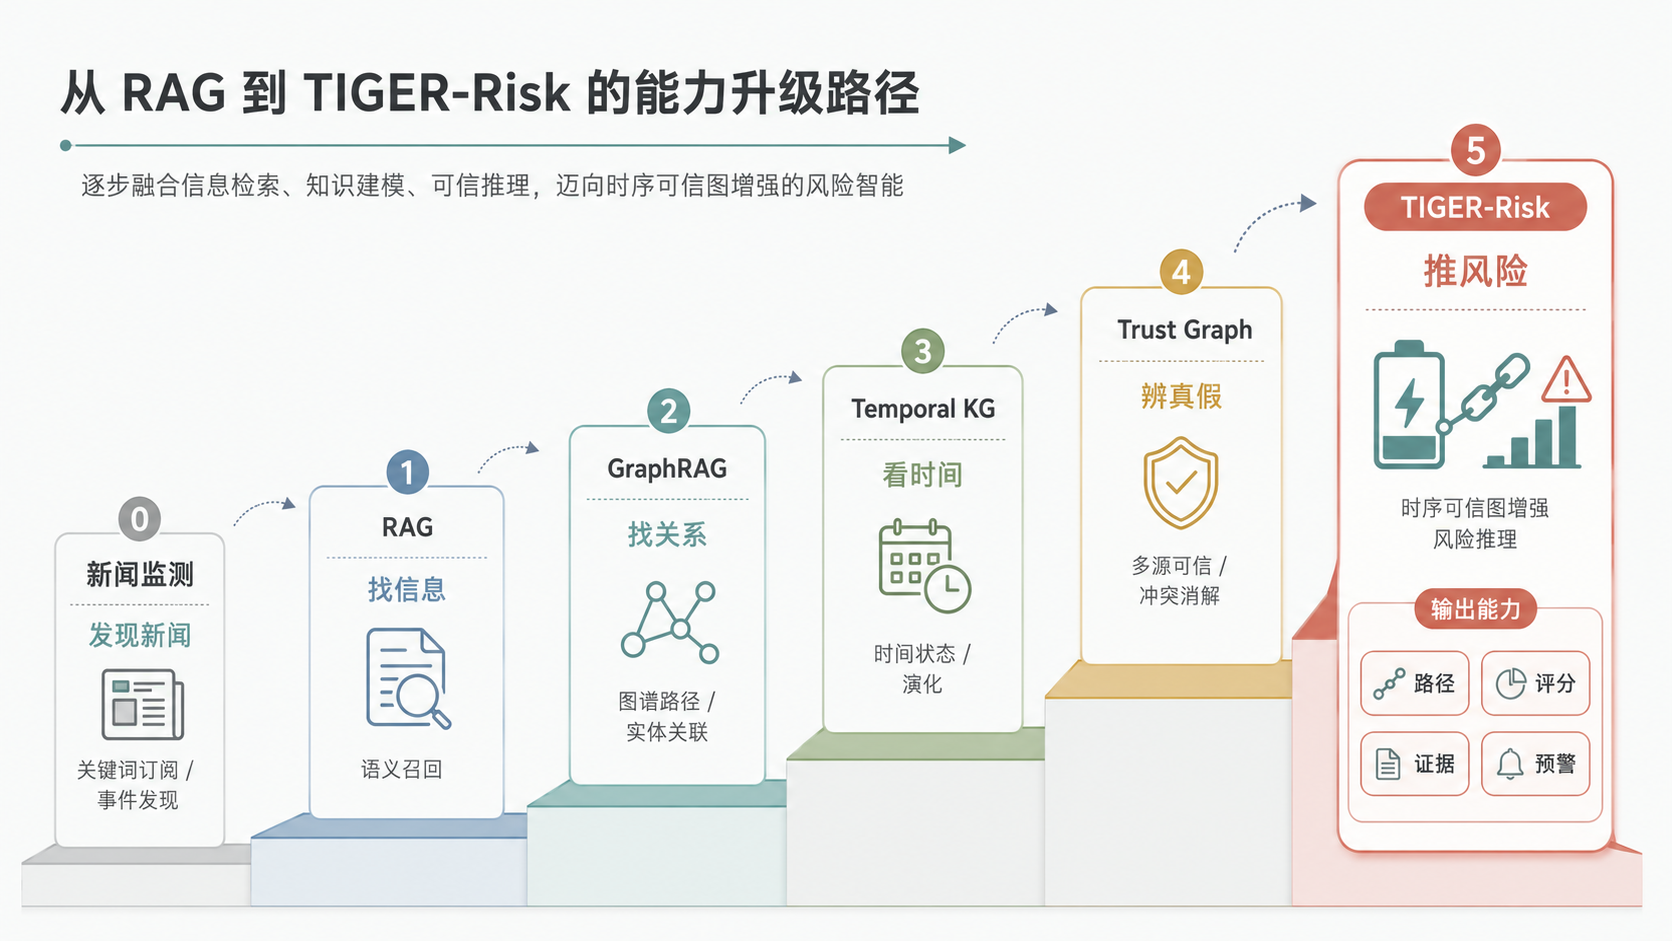
\includegraphics[width=0.95\linewidth]{图3.png}
\caption{项目技术路线在 RAG 体系中的定位}
\label{fig:tech-position}
\end{figure}

综上，本项目技术背景可归纳为一个清晰的升级路径：\term{文本检索解决“找资料”，图谱检索解决“找关系”，时序图谱解决“看当前”，可信图谱解决“辨真假”，图增强大模型解决“会推理”，可视化平台解决“能决策”。}

\subsubsection{团队成员介绍}

项目团队采用三人结构，强调“算法研究—数据工程—系统平台”的紧密闭环。三名成员各自承担独立模块，又通过统一数据结构、接口规范和迭代节奏协同推进，保证项目既有研究创新，也有可运行系统与竞赛演示效果。

\begin{longtable}{p{0.18\textwidth}p{0.22\textwidth}p{0.48\textwidth}}
\toprule
\textbf{角色} & \textbf{署名方式} & \textbf{职责定位与能力包装} \\
\midrule
项目负责人 / 算法架构负责人 & 成员A & 负责整体选题设计、技术路线统筹、时序可信动态图谱建模、风险评分模型设计、核心创新点提炼、项目报告撰写与答辩逻辑构建。该成员重点保证项目具有足够的研究深度和竞赛表达张力，将系统从普通新闻问答提升为图增强风险推理平台。 \\
\midrule
数据与大模型算法负责人 & 成员B & 负责多源异构数据接入、新闻与政策文本清洗、实体识别与消歧、事件结构化抽取 Prompt 设计、跨模态对齐数据集构建、可信度规则与多智能体冲突消解流程实现。该成员重点保证系统具备真实数据处理能力和语义理解能力。 \\
\midrule
工程平台与可视化负责人 & 成员C & 负责后端服务、数据库接口、图谱查询、风险预警接口、前端仪表盘、全球风险地图、产业链图谱视图、事件时间线和 AI 研判报告面板开发。该成员重点保证项目能够形成稳定、直观、可交互、适合现场演示的工程成果。 \\
\bottomrule
\end{longtable}

团队分工并非简单堆叠，而是围绕“一个事件如何进入系统、如何被识别、如何被验证、如何在图中传播、如何被量化、如何被展示”形成端到端闭环。成员 A 负责方法论与指标体系，成员 B 负责数据和模型，成员 C 负责系统和交互。三人共同完成演示案例库、实验对比、项目申报书和答辩材料。团队的优势在于能够把前沿概念转化为可运行工程，把工程系统提炼为可讲述的创新点，把复杂风险推理过程转化为评委能够直观看见的图谱、路径、评分和报告。

\subsection{场景和价值}

\subsubsection{面向专业场景的实战应用价值}

新能源锂电池产业链风险具有高度专业性。通用新闻摘要无法直接服务采购、库存、投研和监管决策，因为决策方真正关心的问题通常不是“发生了什么新闻”，而是“这一新闻是否可信、会影响哪些材料、会沿哪些环节传导、影响窗口大概多久、哪些企业和区域需要重点关注”。本项目面向以下四类专业场景形成实战价值。

\paragraph{新能源电池企业供应链风险管理。}电池企业需要稳定获取锂、镍、钴、石墨等关键材料，并在价格波动、政策变化和运输中断之前提前调整采购与库存策略。系统可以监测上游资源国政策、矿山运行、航运通道、重点供应商和市场价格异常，对高风险节点进行预警，并给出替代供应区域、库存缓冲和持续跟踪建议。

\paragraph{新能源汽车与储能企业生产保障。}下游企业不仅关心电池价格，还关心电池供应稳定性和交付周期。若上游事件可能影响正极材料、电芯产能或电池包交付，系统能够通过产业链路径将风险映射到下游企业和产品环节，帮助企业评估潜在延迟、成本上升和供应商集中度风险。

\paragraph{金融机构与产业投研。}风险事件会影响大宗商品价格、上市公司估值、行业景气度和投资组合风险。系统能够将文本事件、价格信号和图谱关键节点结合起来，形成具有证据链的行业风险研判，为基金、券商、产业研究院和咨询机构提供辅助分析。

\paragraph{政府监管与产业安全监测。}锂电池产业链关系到战略性新兴产业安全。监管部门需要把握关键资源、关键企业、关键技术和关键物流通道的外部风险。系统可形成风险地图、区域热力、时间线与节点排名，帮助发现产业链薄弱环节，提高产业韧性评估与预警能力。

\begin{figure}[H]
\centering
\resizebox{\linewidth}{!}{
\begin{tikzpicture}[
    font=\small,
    % 优化 1：改用 text width 强制限制节点宽度，压缩整体尺寸以完美适配单栏版心
    nodebox/.style={draw=LineGray, rounded corners=2mm, thick, align=center, text width=2.0cm, minimum height=0.9cm, fill=SoftBlue},
    risk/.style={draw=DeepBlue, rounded corners=2mm, very thick, align=center, text width=2.4cm, minimum height=1.0cm, fill=SoftRed},
    arr/.style={-{Latex[length=2.2mm]}, thick, draw=LineGray}
]
% 第一行：由左至右的单线传播
\node[risk] (event) {风险事件\\印尼镍矿政策收紧};
\node[nodebox, right=0.5cm of event] (nickel) {镍矿供应};
\node[nodebox, right=0.5cm of nickel] (sulfate) {硫酸镍};
\node[nodebox, right=0.5cm of sulfate] (precursor) {三元前驱体};
\node[nodebox, right=0.5cm of precursor] (cathode) {三元正极};

% 第二行：向下折返
\node[nodebox, below=0.8cm of cathode] (cell) {动力电池};

% 优化 2：彻底修复拓扑错误。将并行的下游节点改为“上下堆叠”，彻底杜绝连线穿透
\node[nodebox, left=1.0cm of cell, yshift=0.6cm] (ev) {新能源汽车};
\node[nodebox, left=1.0cm of cell, yshift=-0.6cm] (storage) {储能系统};

% 正向流转连线
\draw[arr] (event) -- (nickel);
\draw[arr] (nickel) -- (sulfate);
\draw[arr] (sulfate) -- (precursor);
\draw[arr] (precursor) -- (cathode);
\draw[arr] (cathode) -- (cell);

% 优化 3：使用正交折线 ( |- ) 平行分发至下游，结构极为清晰严谨
\draw[arr] (cell.west) -- ++(-0.5,0) |- (ev.east);
\draw[arr] (cell.west) -- ++(-0.5,0) |- (storage.east);

% 优化 4：拉大距离，将其锚定在首行节点下方 3.0cm 处，彻底越过所有图形区
\node[align=center, below=3.0cm of precursor, text width=13cm] {系统输出：影响路径、关键节点、传播范围、风险分数、置信度、证据来源与应对建议。};
\end{tikzpicture}
}
\caption{新能源锂电池产业链风险传播示意图}
\label{fig:risk-propagation}
\end{figure}

通过上述场景，本项目能够把“开放信息监测”提升为“产业风险智能决策”。这种价值并不依赖单一模型能力，而是来自多源数据、结构化图谱、时间状态、可信机制和风险评分的联合建模。

\subsubsection{面向战略方向的数据价值释放}

新能源锂电池产业链是典型的数据密集型产业链。公开新闻、政策公告、企业公告、海关与航运信息、市场价格、社交媒体和灾害数据长期分散在不同渠道，具有高时效、高噪声、高异构和低结构化的特点。许多数据本身并不稀缺，但真正有价值的是将数据转化为可计算、可追溯、可复用、可推理的知识资产。

本项目通过以下方式释放数据价值。

首先，将非结构化文本转化为结构化风险事件。系统通过信息抽取模型或大模型 Prompt，将新闻段落解析为事件类型、事件主体、发生时间、地点、影响对象、严重度、状态、来源和摘要等字段。这样，文本不再只是可读材料，而成为可被检索、比较、聚类和推理的事件对象。

其次，将事件映射到产业链知识图谱。一个事件只有被挂接到材料、企业、国家、物流节点和产业环节上，才具备产业意义。例如，“某港口拥堵”如果无法连接到“电池材料运输通道”和“欧洲电池供应链”，则只能作为地理新闻存在；一旦映射到图谱，它就可以参与风险传播计算。

再次，将多源证据转化为可信度资产。不同来源报道同一事件时，系统会根据来源信誉度、时间接近度、实体匹配度和多源一致性形成置信度。长期运行后，系统能够积累来源表现、事件冲突模式和证据链结构，为后续预警提供更稳定的可信基础。

最后，将历史事件转化为演化知识。黑天鹅风险往往不是瞬时生成，而是由弱信号逐步升级。项目通过事件状态机保存从 rumor 到 confirmed、escalating、active、mitigating、resolved 或 invalidated 的演化过程，使系统能够分析“风险如何出现、如何扩散、如何缓解、哪些早期信号具有预警价值”。

因此，本项目的数据价值并非简单“采集更多数据”，而是建立一套从原始数据到结构化事件、从事件到图谱、从图谱到推理、从推理到决策报告的价值转化链条。该链条能够使新能源产业链开放数据从“信息材料”转化为“风险智能资产”。

\subsubsection{面向复杂语义的智能理解能力}

产业链风险语义具有复杂性，主要体现在五个方面。第一，同一实体存在多种表达，例如“刚果金”“DRC”“Democratic Republic of Congo”可能指向同一国家节点。第二，同一事件存在不同粒度，例如“出口限制”“政策收紧”“配额调整”“许可证审批变严”都可能属于政策风险。第三，同一关系具有时间变化，例如“计划投资”“正在建设”“推迟投产”“取消项目”不能被视为同一状态。第四，多源信息存在冲突，例如主流媒体称“供应受限”，企业公告称“暂无实质影响”。第五，风险影响具有隐含传播路径，文本中未必直接出现“电池成本上升”，但图谱路径可能显示上游材料紧张会传导至中游正极和下游电芯。

本项目通过“语义抽取 + 实体消歧 + 时序对齐 + 信任评估 + 图谱传播”的组合增强复杂语义理解能力。其关键不是让大模型凭常识自由发挥，而是让大模型在结构化证据中生成受约束的答案。系统在生成报告时会明确给出证据来源、事件状态、置信度、影响路径和风险分数，使回答可核查、可解释、可复现。

在竞赛展示中，这种智能理解能力可以通过现场问题体现。例如，评委输入“最近某国限制石墨出口会不会影响欧洲储能系统”，系统应当完成以下推理链：识别“某国”和“石墨”相关事件，判断事件时间与状态，检索政策公告和媒体证据，映射到“负极材料—电芯—储能系统”路径，计算石墨节点关键性和传播范围，结合来源置信度输出风险评分，最后生成一份带有证据链和后续监控建议的研判报告。该过程比普通问答系统更能体现“复杂语义理解 + 行业知识推理 + 工程落地”的综合能力。

\subsection{所需支持}

\subsubsection{算力支持}

本项目采用“轻量规则图算法 + 可插拔大模型服务 + 小规模向量检索”的工程路线，避免完全依赖大规模模型训练，保证竞赛阶段可实现、可演示、可迭代。项目所需算力主要包括四类。

\paragraph{一、文本抽取与报告生成算力（LLM 推理）。}事件抽取、摘要生成和研判报告生成使用云端大模型 API 或本地开源模型。本地推理建议配置 NVIDIA \textbf{A800}（80GB 显存），可高效运行 70B 级大模型推理。若需进行 LoRA 微调或批量抽取，A800 的大显存可支持大 batch 处理。竞赛演示阶段可采用“离线样例库 + 在线补充抽取”混合模式，降低实时算力压力。

\paragraph{二、向量检索与语义编码算力（嵌入编码）。}新闻文本、事件摘要、政策公告和证据片段需要编码为向量。该部分使用 NVIDIA \textbf{RTX 5080} 进行嵌入编码，可高效运行中文/英文双语嵌入模型的批处理。由于项目数据规模以比赛演示和原型验证为主，百万级以下文本向量可通过 pgvector 向量数据库完成。

\paragraph{三、图计算与风险传播算力。}图谱节点包括国家、材料、企业、产业环节、物流通道和事件节点，边包括供应、依赖、影响、政策、运输、制裁和证据关系。PageRank、中心性、最短路径、影响子图搜索等计算可在 CPU 上完成。若后续扩展到大规模产业图谱，可引入图数据库或分布式图计算框架。

\paragraph{四、前端可视化与实时服务算力。}可视化平台需要支持全球地图、动态图谱、时间线、风险排行榜、报告面板和多源事件刷新。建议使用一台 4 核以上 CPU、16GB 以上内存的服务器进行原型部署；若同时支持多人访问和持续数据采集，建议提升至 8 核 CPU、32GB 内存和独立存储空间。

\subsubsection{硬件支持}

项目硬件支持重点在于保证系统稳定运行、演示流畅和数据持续采集。建议配置如下：

\begin{longtable}{p{0.26\textwidth}p{0.62\textwidth}}
\toprule
\textbf{硬件或环境} & \textbf{用途说明} \\
\midrule
开发工作站 & 配备 Intel \textbf{酷睿 Ultra 9 285K}、32GB 以上内存，用于代码开发、前端调试、数据清洗、图谱构建和本地演示。 \\
\midrule
GPU 服务器 & NVIDIA \textbf{A800}（80GB，LLM 推理）+ \textbf{RTX 5080}（嵌入编码），用于大模型本地推理、批量事件抽取和 Embedding 编码。 \\
\midrule
应用部署服务器 & 用于后端 API、数据库、定时采集任务、风险评分服务和 Web 前端展示。建议使用 Linux 环境，便于部署 Node.js、Python、图数据库和向量数据库。 \\
\midrule
展示设备 & 用于答辩现场演示全球风险地图、产业链动态图谱、事件时间线和 AI 研判报告。建议准备离线演示数据，避免现场网络波动影响展示。 \\
\bottomrule
\end{longtable}

硬件建设的核心原则是“优先保证系统闭环，其次追求模型规模”。项目可以先用规则、图算法和 API 模型实现高完成度原型，再根据时间和资源逐步引入更强的本地大模型与增量学习能力。

\subsubsection{数据支持}

本项目需要的数据可以分为基础产业链知识、实时开放事件、市场与价格信号、地理物流数据、可信度元数据和人工验证样例六类。

\paragraph{基础产业链知识。}包括国家、区域、矿产资源、材料、产业环节、企业、物流节点和产品应用之间的静态关系，是构建初始知识图谱的基础。例如智利、阿根廷、澳大利亚、印尼、刚果金等资源相关国家；锂、镍、钴、石墨、碳酸锂、氢氧化锂、硫酸镍等关键材料；采矿、冶炼、前驱体、正极、负极、电芯、电池包、整车和储能等产业环节。

\paragraph{实时开放事件数据。}包括全球新闻 RSS、政府公告、行业媒体、企业公告、制裁名单、贸易政策、航运事件、自然灾害和社交媒体舆情。该部分用于发现新增风险事件，是系统保持时效性的核心。

\paragraph{市场与价格信号。}包括锂、镍、钴等金属价格，相关企业股价，宏观经济指标和行业价格数据。价格异常往往是风险事件影响市场的外部表现，可作为风险验证和辅助评分依据。

\paragraph{地理物流与灾害数据。}包括港口、航线、海峡、地震、洪水、火灾、极端天气等信息。锂电池产业链具有强跨境运输属性，物流中断和自然灾害可能造成供应延迟或成本上升。

\paragraph{可信度元数据。}包括来源类型、历史可信度、自动化接入方式、是否官方、是否需要人工核验等信息。该部分用于 Trust Graph 建模，使系统能够区分官方公告、主流媒体、行业媒体、社交媒体和匿名来源。

\paragraph{人工验证样例。}竞赛阶段应构建 30 至 50 条典型风险事件样例，覆盖政策变化、制裁风险、供应中断、物流中断、自然灾害、价格异常、罢工事件、地缘冲突和环保监管等类型。样例库既用于系统调试，也用于现场演示和指标评估，确保系统在比赛环境下稳定输出。

% ====================== 2 项目规划 ======================
\section{项目规划}
\subsection{大模型驱动的数据集语义检索与智能推荐技术}

本项目的技术核心可以概括为“大模型理解语义、图谱组织知识、时序保证有效、可信机制过滤噪声、图算法支撑推理、可视化承载决策”。在实现层面，系统围绕多源数据集的语义检索与智能推荐构建三项关键技术：基于数据增强的多模态特征提取、基于多层一致性的多模态特征融合，以及面向风险推理任务的大模型适应技术。

\subsubsection{基于数据增强的多模态特征提取技术}

多源风险数据具有噪声高、表达不一致、字段缺失和时效敏感等特点。为了使系统能够稳定识别风险事件，项目首先构建多模态特征提取模块，将不同来源数据转化为统一的事件表示。对于一条原始信息 $x_i$，系统提取文本语义特征 $\bm{h}^{text}_i$、实体链接特征 $\bm{h}^{entity}_i$、时间特征 $\bm{h}^{time}_i$、来源可信特征 $\bm{h}^{trust}_i$、图谱位置特征 $\bm{h}^{graph}_i$ 和市场信号特征 $\bm{h}^{market}_i$，形成综合表示：
\begin{equation}
\bm{z}_i = \left[\bm{h}^{text}_i;\bm{h}^{entity}_i;\bm{h}^{time}_i;\bm{h}^{trust}_i;\bm{h}^{graph}_i;\bm{h}^{market}_i\right].
\end{equation}

\paragraph{文本语义特征。}系统使用大模型或轻量信息抽取模型识别事件类型、主体、客体、动作、地点、时间、影响对象和摘要。为增强鲁棒性，系统在 Prompt 中加入行业词表、实体别名、事件类型定义和输出格式约束，避免模型生成过于自由的字段。

\paragraph{实体链接特征。}系统将文本中的企业、国家、材料、产业环节和物流节点映射到知识图谱节点。实体链接不仅依赖字符串匹配，还结合别名表、上下文语义和产业链类型约束。例如，“镍”在普通语境中可能只是金属名，但在本项目中会进一步连接到“镍矿—硫酸镍—三元前驱体—三元正极”的产业链路径。

\paragraph{时间特征。}系统抽取事件发生时间、报道时间、关系生效时间、关系失效时间和状态更新时间。对缺失时间的事件，通过来源发布时间和文本上下文进行保守估计，并标记时间置信度。时间特征用于过滤过期信息和计算时间新鲜度。

\paragraph{来源可信特征。}系统根据来源类型赋予基础信誉度，并根据多源一致性、实体匹配准确度和时间接近度进行修正。官方公告、政府机构、国际组织、市场数据源、主流媒体、行业媒体和社交媒体对应不同基础权重。

\paragraph{图谱位置特征。}当事件被映射到产业链图谱后，系统计算相关节点的度中心性、PageRank、中介中心性、所属社区和上下游距离。图谱位置决定风险传播潜力，是区别“普通新闻”和“关键产业风险”的重要特征。

\paragraph{市场信号特征。}若风险事件与金属价格、企业股价或行业指数存在时间相关性，系统将价格涨跌、波动率、异常程度和趋势方向作为辅助特征，用于验证事件影响和增强风险评分。

数据增强主要体现在三个方面：一是通过同义词、别名、翻译和行业表达扩充实体识别范围；二是通过事件模板和状态机增强模型对不同风险类型的抽取稳定性；三是通过历史案例扩充风险传播路径和报告生成示例。该设计能够在样本规模有限的竞赛阶段显著提升系统表现。

\begin{figure}[H]
\centering
\begin{tikzpicture}[
    font=\small,
    source/.style={draw=LineGray, rounded corners=2mm, thick, align=center, minimum width=2.55cm, minimum height=0.85cm, fill=SoftBlue},
    feat/.style={draw=LineGray, rounded corners=2mm, thick, align=center, minimum width=2.7cm, minimum height=0.85cm, fill=SoftOrange},
    core/.style={draw=DeepBlue, rounded corners=2mm, very thick, align=center, minimum width=4.0cm, minimum height=1.05cm, fill=Mint},
    arr/.style={-{Latex[length=2.2mm]}, thick, draw=LineGray}
]
\node[source] (s1) {新闻/公告};
\node[source, below=0.25cm of s1] (s2) {市场价格};
\node[source, below=0.25cm of s2] (s3) {航运地理};
\node[source, below=0.25cm of s3] (s4) {灾害天气};
\node[source, below=0.25cm of s4] (s5) {社交舆情};

\node[feat, right=1.2cm of s1] (f1) {文本语义};
\node[feat, right=1.2cm of s2] (f2) {实体链接};
\node[feat, right=1.2cm of s3] (f3) {时间状态};
\node[feat, right=1.2cm of s4] (f4) {来源可信};
\node[feat, right=1.2cm of s5] (f5) {市场信号};

\node[core, right=1.25cm of f3] (z) {统一事件表示 $\bm{z}_i$\\用于检索、聚类、图谱挂接与评分};

\foreach \a/\b in {s1/f1,s2/f2,s3/f3,s4/f4,s5/f5}{\draw[arr] (\a) -- (\b);}
\foreach \b in {f1,f2,f3,f4,f5}{\draw[arr] (\b.east) -- (z.west);}
\end{tikzpicture}
\caption{多源风险数据的特征提取与统一表示}
\label{fig:feature-extraction}
\end{figure}

\subsubsection{基于多层一致性的多模态特征融合技术}

多模态融合的难点不在于把所有数据简单拼接，而在于判断不同模态之间是否相互支持、相互冲突或相互补充。本项目提出多层一致性融合思路，从实体一致性、事件一致性、时间一致性、来源一致性和图谱一致性五个层面降低噪声影响。

\paragraph{实体一致性。}不同来源是否指向同一国家、企业、材料或物流节点。若新闻 A 提到“印尼镍矿出口限制”，新闻 B 提到“Indonesia tightens nickel export permit”，系统需要判断它们属于同一实体和相近事件，而不是分别存储为孤立事件。

\paragraph{事件一致性。}不同报道是否描述同一风险类型、同一动作和相近影响对象。若一个来源称“政策收紧”，另一个来源称“出口审批延迟”，系统需要判断二者是否属于同一政策变化事件簇。

\paragraph{时间一致性。}事件发生时间、报道时间和后续更新是否构成合理演化链。若旧新闻已被新公告澄清，系统应优先采用新状态，而不能将过期高风险信息继续作为当前判断依据。

\paragraph{来源一致性。}高可信来源之间是否互相印证，低可信来源是否被高可信来源确认或否认。系统不是简单统计报道数量，而是根据来源权重形成加权一致性。

\paragraph{图谱一致性。}事件影响路径是否符合产业链结构。若某事件文本声称影响某下游环节，但图谱中缺乏合理传播路径，系统应降低置信度或要求更多证据。

综合置信度可表示为：
\begin{equation}
C(e)=w_s C_{source}(e)+w_m C_{multi}(e)+w_l C_{link}(e)+w_t C_{time}(e)+w_g C_{graph}(e),
\end{equation}
其中 $C_{source}$ 表示来源信誉度，$C_{multi}$ 表示多源一致性，$C_{link}$ 表示实体链接准确度，$C_{time}$ 表示时间接近度与有效性，$C_{graph}$ 表示产业链路径合理性。项目原型阶段可设置 $w_s=0.35,w_m=0.25,w_l=0.15,w_t=0.15,w_g=0.10$，后续可根据人工验证集进行调优。

\begin{figure}[H]
\centering
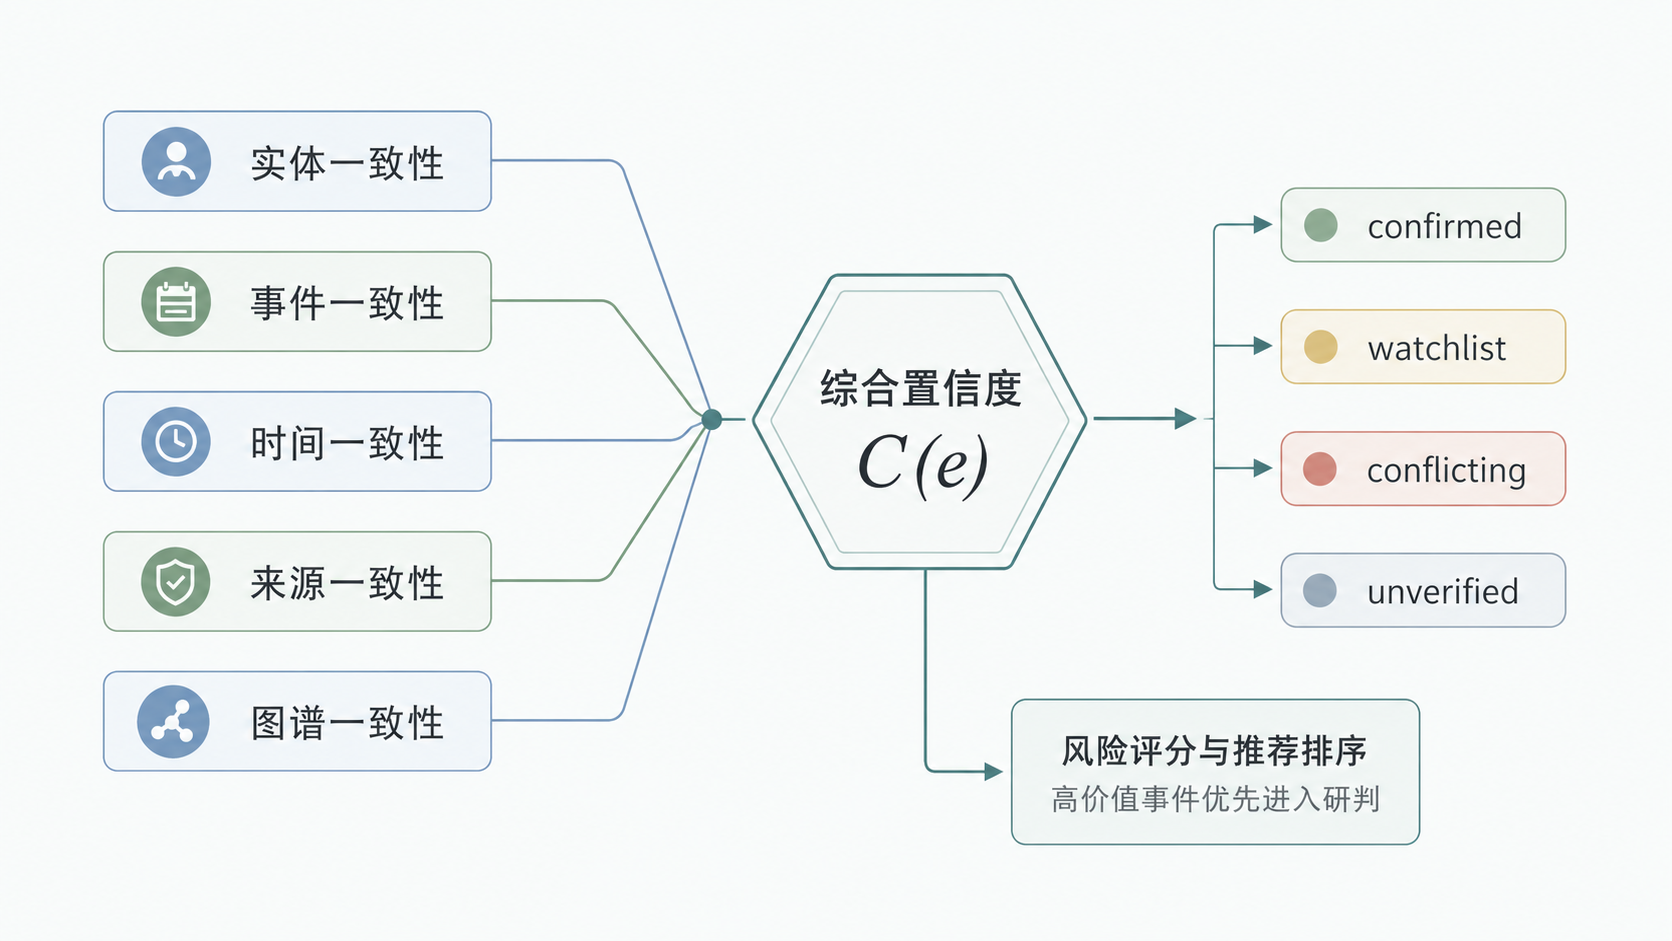
\includegraphics[width=0.85\linewidth]{图6.png}
\caption{多层一致性驱动的可信融合机制}
\label{fig:consistency-fusion}
\end{figure}

该融合机制具有两个优势。第一，它能够使系统在开放数据环境下保持稳健，不会被单一噪声来源轻易误导。第二，它能够将“为什么相信这一事件”显式表达出来，便于在项目答辩中展示系统的可解释性。

\subsubsection{大模型与多模态的检索推荐任务适应技术}

本项目中的大模型主要承担四类任务：结构化抽取、语义归一、冲突解释和报告生成。为了避免大模型幻觉，系统采用“\term{大模型生成候选，规则和图谱进行约束，证据链进行校验，评分模型进行量化}”的适应策略。

\paragraph{结构化抽取适应。}系统设计领域 Prompt，将原始文本转换为标准事件字段。Prompt 中包含事件类型集合、实体类型集合、状态集合、输出字段约束和缺失值处理规则。模型输出后，系统通过 JSON Schema、实体词表、时间格式和图谱节点校验进行过滤。

\paragraph{语义归一适应。}大模型用于将不同表述归一到统一风险类型和产业链节点。例如，“出口审批趋严”“限制原矿出口”“配额下调”可归入政策变化或供应限制；“battery material”“cathode precursor”“三元前驱体”可通过上下文映射到对应图谱节点。

\paragraph{冲突解释适应。}当不同来源存在冲突时，大模型不直接裁决真假，而是被要求列出冲突点、各自证据、来源类型和可能解释。随后由 Trust Graph 根据权重和一致性给出状态标签。这样既发挥大模型语言理解能力，又避免其替代证据判断。

\paragraph{报告生成适应。}报告生成阶段输入不是原始大段新闻，而是经过检索、图谱推理和评分后的结构化上下文，包括事件摘要、证据来源、影响路径、风险分数、置信度、历史演化和后续监控项。模型需按固定模板生成研判报告，保证结果完整、可追溯、可复核。

\begin{figure}[H]
\centering
\begin{tikzpicture}[
    font=\small,
    agent/.style={draw=LineGray, rounded corners=2mm, thick, align=center, minimum width=2.6cm, minimum height=0.9cm, fill=SoftBlue},
    center/.style={draw=DeepBlue, rounded corners=2mm, very thick, align=center, minimum width=3.6cm, minimum height=1.1cm, fill=SoftPurple},
    outbox/.style={draw=LineGray, rounded corners=2mm, thick, align=center, minimum width=3.1cm, minimum height=0.9cm, fill=Mint},
    arr/.style={-{Latex[length=2.2mm]}, thick, draw=LineGray}
]
\node[center] (ctx) {结构化证据上下文\\图谱路径 + 置信度 + 时间状态};
\node[agent, above left=0.75cm and 1.0cm of ctx] (a1) {抽取 Agent};
\node[agent, above=0.75cm of ctx] (a2) {检索 Agent};
\node[agent, above right=0.75cm and 1.0cm of ctx] (a3) {可信度 Agent};
\node[agent, below left=0.75cm and 1.0cm of ctx] (a4) {推理 Agent};
\node[agent, below=0.75cm of ctx] (a5) {质询 Agent};
\node[agent, below right=0.75cm and 1.0cm of ctx] (a6) {报告 Agent};
\node[outbox, right=1.35cm of ctx] (out) {可解释研判输出\\评分、路径、证据、建议};
\foreach \x in {a1,a2,a3,a4,a5,a6}{\draw[arr] (\x) -- (ctx);}
\draw[arr] (ctx) -- (out);
\end{tikzpicture}
\caption{大模型多智能体协同适应框架}
\label{fig:multi-agent}
\end{figure}

检索推荐排序方面，系统将候选事件的推荐优先级定义为：
\begin{equation}
P(e)=\lambda_1 R(e)+\lambda_2 C(e)+\lambda_3 K(v_e)+\lambda_4 F(e,t)+\lambda_5 U(e),
\end{equation}
其中 $R(e)$ 为事件风险分数，$C(e)$ 为置信度，$K(v_e)$ 为相关节点关键性，$F(e,t)$ 为时间新鲜度，$U(e)$ 为用户场景相关性。对于企业用户，系统可提高供应链影响权重；对于投研用户，可提高价格和企业关联权重；对于监管用户，可提高区域与战略资源权重。该机制使系统具备面向不同用户的智能推荐能力。

\subsection{多模态数据集构建与语义标注}

高质量数据集是项目可靠运行和竞赛评估的基础。本项目计划构建“开放数据采集 + 行业知识整理 + 人工样例标注 + 模型辅助扩充”的多模态数据集。数据集并不追求盲目大规模，而强调场景覆盖、字段规范、证据链完整、风险类型均衡和可用于演示评估。

\subsubsection{跨模态对齐训练数据集构建}

跨模态对齐训练数据集用于训练或调试事件抽取、实体链接、语义检索、风险分类和报告生成模块。数据集以“事件”为基本单元，每个事件包含原始文本、结构化字段、图谱节点、证据来源、时间状态和风险标签。

\paragraph{数据来源。}训练数据主要来自行业新闻 RSS、政策公告、企业公告、市场价格摘要、制裁名单、航运事件、气候灾害和社交媒体公开信息。项目会优先选择与锂、镍、钴、石墨、碳酸锂、氢氧化锂、硫酸镍、正极材料、负极材料、电芯制造、储能系统和新能源汽车相关的数据。

\paragraph{事件类型体系。}项目定义九类核心风险事件：政策变化、制裁风险、供应中断、物流中断、自然灾害、价格异常、罢工事件、地缘冲突和环保监管。必要时扩展企业经营风险、技术路线变化、贸易摩擦和市场需求异常等类型。

\paragraph{实体类型体系。}实体类型包括国家/地区、企业、材料、产品、产业环节、物流节点、政策机构、市场指标和事件。每个实体维护唯一 ID、中文名、英文名、别名、类型、关键性和证据来源。

\paragraph{关系类型体系。}关系类型包括供应、依赖、影响、运输、生产、监管、制裁、替代、价格影响、证据支持和事件演化。每条关系包含开始时间、结束时间、状态、置信度和证据列表。

\paragraph{标注字段。}跨模态对齐样本建议采用如下字段：
\begin{longtable}{p{0.22\textwidth}p{0.64\textwidth}}
\toprule
\textbf{字段} & \textbf{说明} \\
\midrule
事件编号 & 每个风险事件的唯一标识，用于追踪聚类、版本更新和证据合并。 \\
事件类型 & policy\_change、sanction、supply\_disruption、logistics\_disruption、natural\_disaster、price\_spike 等。 \\
事件主体 & 触发风险的国家、机构、企业、港口、矿山或材料。 \\
影响对象 & 受影响的材料、企业、产业环节、区域或产品。 \\
发生时间 & 事件实际发生时间；若未知，则记录报道时间并降低时间置信度。 \\
状态标签 & rumor、confirmed、escalating、active、mitigating、resolved、invalidated。 \\
严重度 & 0 至 1 之间的事件影响强度，可由规则、人工标注或模型辅助估计。 \\
来源列表 & 支持该事件的新闻、公告、市场数据或社交媒体来源。 \\
来源可信度 & 根据来源类型、多源一致性和历史可靠性计算。 \\
图谱映射节点 & 事件对应的材料、企业、国家、环节和物流节点 ID。 \\
传播路径 & 由图谱搜索得到的上下游影响链。 \\
风险等级 & 低、中、高、紧急四级标签。 \\
人工备注 & 用于说明冲突信息、特殊背景和标注不确定性。 \\
\bottomrule
\end{longtable}

\paragraph{数据增强策略。}为了增强训练样本多样性，系统会对事件文本进行同义改写、跨语言翻译、实体别名替换、时间表达转换和摘要压缩。例如“export restriction”可扩展为“出口限制”“出口管制”“出口许可证收紧”等表达；“Lithium Carbonate”可与“碳酸锂”对齐；“three months later”需转化为明确时间区间。增强样本必须保留原始语义，不改变事实关系。

\paragraph{质量控制。}数据标注采用“模型预标注 + 人工校正 + 规则校验”的流程。模型负责初步抽取，规则负责检查字段完整性、实体是否存在、时间格式是否正确，人工负责处理高风险、高冲突和高不确定样本。对于比赛阶段，优先保证 30 至 50 条高质量样例覆盖典型演示场景，再逐步扩充到数百条事件。

\begin{figure}[H]
\centering
\begin{tikzpicture}[
    font=\small,
    stepbox/.style={draw=LineGray, rounded corners=2mm, thick, align=center, minimum width=3.0cm, minimum height=0.95cm, fill=SoftBlue},
    check/.style={draw=DeepBlue, rounded corners=2mm, very thick, align=center, minimum width=3.0cm, minimum height=0.95cm, fill=SoftOrange},
    data/.style={draw=LineGray, rounded corners=2mm, thick, align=center, minimum width=3.1cm, minimum height=0.95cm, fill=Mint},
    arr/.style={-{Latex[length=2.2mm]}, thick, draw=LineGray}
]
\node[stepbox] (raw) {原始多源数据};
\node[stepbox, right=0.8cm of raw] (extract) {模型预抽取};
\node[check, right=0.8cm of extract] (validate) {规则校验};
\node[check, right=0.8cm of validate] (human) {人工复核};
\node[data, below=0.85cm of validate] (dataset) {跨模态对齐训练集\\事件 + 实体 + 时间 + 图谱 + 证据};
\draw[arr] (raw) -- (extract);
\draw[arr] (extract) -- (validate);
\draw[arr] (validate) -- (human);
\draw[arr] (human.south) -- (dataset.east);
\draw[arr, dashed] (dataset.west) -- (extract.south);
\end{tikzpicture}
\caption{跨模态对齐训练数据集构建流程}
\label{fig:dataset-construction}
\end{figure}

\subsubsection{多模态语义检索验证集构建}

验证集用于评估系统是否真正具备语义检索、图谱推理和风险推荐能力。与普通问答评测不同，本项目验证集需要覆盖“文本相关性、实体对齐正确性、时间有效性、证据可信性、影响路径合理性和报告可解释性”。

\paragraph{验证问题设计。}项目计划构建四类验证问题。

\begin{itemize}
\item \term{事实检索类问题：}例如“过去一个月与锂矿罢工相关的事件有哪些？”用于评估系统召回相关事件的能力。
\item \term{时序判断类问题：}例如“某公司投资某矿山的关系当前是否仍有效？”用于评估系统识别过期或失效关系的能力。
\item \term{传播推理类问题：}例如“红海航运中断会影响哪些锂电池产业链环节？”用于评估图谱路径搜索和上下游影响推理能力。
\item \term{可信冲突类问题：}例如“不同来源对某政策影响存在冲突时，系统应如何判断？”用于评估 Trust Graph 与多 Agent 冲突消解能力。
\end{itemize}

\paragraph{验证标签设计。}每个验证样本包含标准答案、相关证据、正确图谱路径、应排除的干扰证据、时间状态和置信度范围。对于报告生成类问题，采用人工评分方式评价完整性、准确性、可解释性、证据引用和建议可操作性。

\paragraph{核心评价指标。}项目可采用以下指标进行竞赛材料包装与原型评估。
\begin{longtable}{p{0.25\textwidth}p{0.58\textwidth}p{0.10\textwidth}}
\toprule
\textbf{指标} & \textbf{含义} & \textbf{方向} \\
\midrule
事件召回率 & 系统是否检索到与问题相关的关键风险事件。 & 越高越好 \\
图谱路径准确率 & 生成的影响路径是否符合产业链结构与标注答案。 & 越高越好 \\
时间有效性判断准确率 & 系统是否正确识别事件当前状态、过期关系和后续修正。 & 越高越好 \\
可信冲突识别率 & 系统是否发现多源冲突并给出合理状态标签。 & 越高越好 \\
幻觉率 & 报告中无证据支持或图谱不支持的结论比例。 & 越低越好 \\
解释完整度 & 报告是否包含风险分数、证据来源、传播路径和建议。 & 越高越好 \\
响应时延 & 从用户提交问题到返回结果的时间。 & 越低越好 \\
\bottomrule
\end{longtable}

\paragraph{对比基线。}为了突出项目创新性，验证集可设置三个基线：普通关键词检索、普通向量 RAG、静态 GraphRAG。对比重点不是绝对大规模指标，而是展示系统在复杂跨文本推理、过期信息过滤、冲突来源消解和产业链路径解释方面的优势。建议在报告中使用“案例评估 + 人工评分 + 小规模量化”的方式呈现，既保证可信度，也适合竞赛节奏。

\paragraph{典型验证案例。}验证集可覆盖以下演示案例：印尼镍矿出口政策变化、智利锂矿罢工、红海航运中断、刚果金钴矿政策调整、欧盟电池法案更新、石墨出口管制、极端天气影响澳大利亚矿山运输、关键企业被制裁或列入限制名单等。这些案例具备产业链传播路径清晰、新闻证据丰富、现场展示效果强的特点。

\subsection{多模态语义检索与知识推荐系统平台构建}

系统平台是项目成果的集中体现。平台不是单一网页或问答框，而是一个从数据接入、事件抽取、图谱构建、可信评估、风险推理、报告生成到可视化展示的完整闭环。平台建设目标是让评委能够直观看到：系统如何从一条新闻进入，到形成一张动态风险图谱，再到输出一份带评分、路径和证据的行业研判报告。

\subsubsection{检索推荐流程与查询逻辑}

平台查询逻辑采用“用户问题解析—多路召回—证据融合—图谱推理—风险评分—报告生成”的流程。

\paragraph{用户问题解析。}系统首先识别用户查询中的实体、时间范围、风险类型和目标场景。例如“如果印尼继续收紧镍矿出口，对国内三元正极企业有什么影响？”这一问题包含国家实体“印尼”、材料实体“镍矿”、风险类型“政策收紧/供应限制”、影响对象“三元正极企业”和隐含时间条件“当前至未来一段时间”。

\paragraph{多路召回。}系统同时执行文本向量召回、关键词召回、图谱邻域召回、时间窗口召回和可信来源优先召回。多路召回能够提高覆盖率，避免单一向量相似度漏掉专业表达或结构相关信息。

\paragraph{证据融合。}召回结果经过去重、聚类、来源打分、冲突识别和时间状态判断，形成结构化证据包。证据包包括支持证据、冲突证据、低可信证据和历史修正证据。

\paragraph{图谱推理。}系统将事件节点挂接到产业链图谱，搜索上下游影响路径，计算节点关键性和传播范围。若事件关联高关键性节点或传播路径较长，系统自动提高风险优先级。

\paragraph{风险评分。}风险评分采用可解释加权模型：
\begin{equation}
\text{RiskScore}(e)=100\times(0.35S_e+0.25K_v+0.20C_e+0.15P_e+0.05F_t),
\end{equation}
其中 $S_e$ 为事件严重度，$K_v$ 为受影响节点关键性，$C_e$ 为来源置信度，$P_e$ 为传播影响范围，$F_t$ 为时间新鲜度。风险分数映射为四级：0--30 低风险，31--60 中风险，61--80 高风险，81--100 紧急风险。

\paragraph{报告生成。}大模型根据结构化上下文生成报告，报告必须包含事件摘要、风险类型、当前状态、风险分数、置信度、影响路径、关键证据、历史演化、潜在影响、应对建议和后续监控重点。

\begin{figure}[H]
\centering
\begin{tikzpicture}[
    font=\small,
    stepbox/.style={draw=LineGray, rounded corners=2mm, thick, align=center, minimum width=2.7cm, minimum height=0.9cm, fill=SoftBlue},
    core/.style={draw=DeepBlue, rounded corners=2mm, very thick, align=center, minimum width=3.0cm, minimum height=0.95cm, fill=SoftPurple},
    outbox/.style={draw=LineGray, rounded corners=2mm, thick, align=center, minimum width=3.0cm, minimum height=0.9cm, fill=Mint},
    arr/.style={-{Latex[length=2.2mm]}, thick, draw=LineGray}
]
\node[stepbox] (q) {用户查询};
\node[stepbox, right=0.55cm of q] (parse) {意图解析\\实体/时间/场景};
\node[stepbox, right=0.55cm of parse] (retrieve) {多路召回\\文本/图谱/时间/来源};
\node[core, right=0.55cm of retrieve] (fusion) {证据融合\\去重/聚类/冲突消解};
\node[core, below=0.75cm of fusion] (reason) {图谱推理\\路径/关键性/传播范围};
\node[outbox, left=0.55cm of reason] (score) {风险评分\\等级/置信度};
\node[outbox, left=0.55cm of score] (report) {研判报告\\证据链/建议};
\draw[arr] (q) -- (parse);
\draw[arr] (parse) -- (retrieve);
\draw[arr] (retrieve) -- (fusion);
\draw[arr] (fusion) -- (reason);
\draw[arr] (reason) -- (score);
\draw[arr] (score) -- (report);
\end{tikzpicture}
\caption{平台检索推荐流程与查询逻辑}
\label{fig:query-flow}
\end{figure}

\subsubsection{平台架构设计与模块分层}

平台整体采用六层架构：多源数据接入层、事件抽取与结构化层、时序动态图谱构建层、可信度评估与冲突消解层、风险传播推理与评分层、可视化展示与智能报告生成层。该分层既便于工程实现，也便于在项目报告和答辩中展示技术完整性。

\begin{figure}[H]
\centering
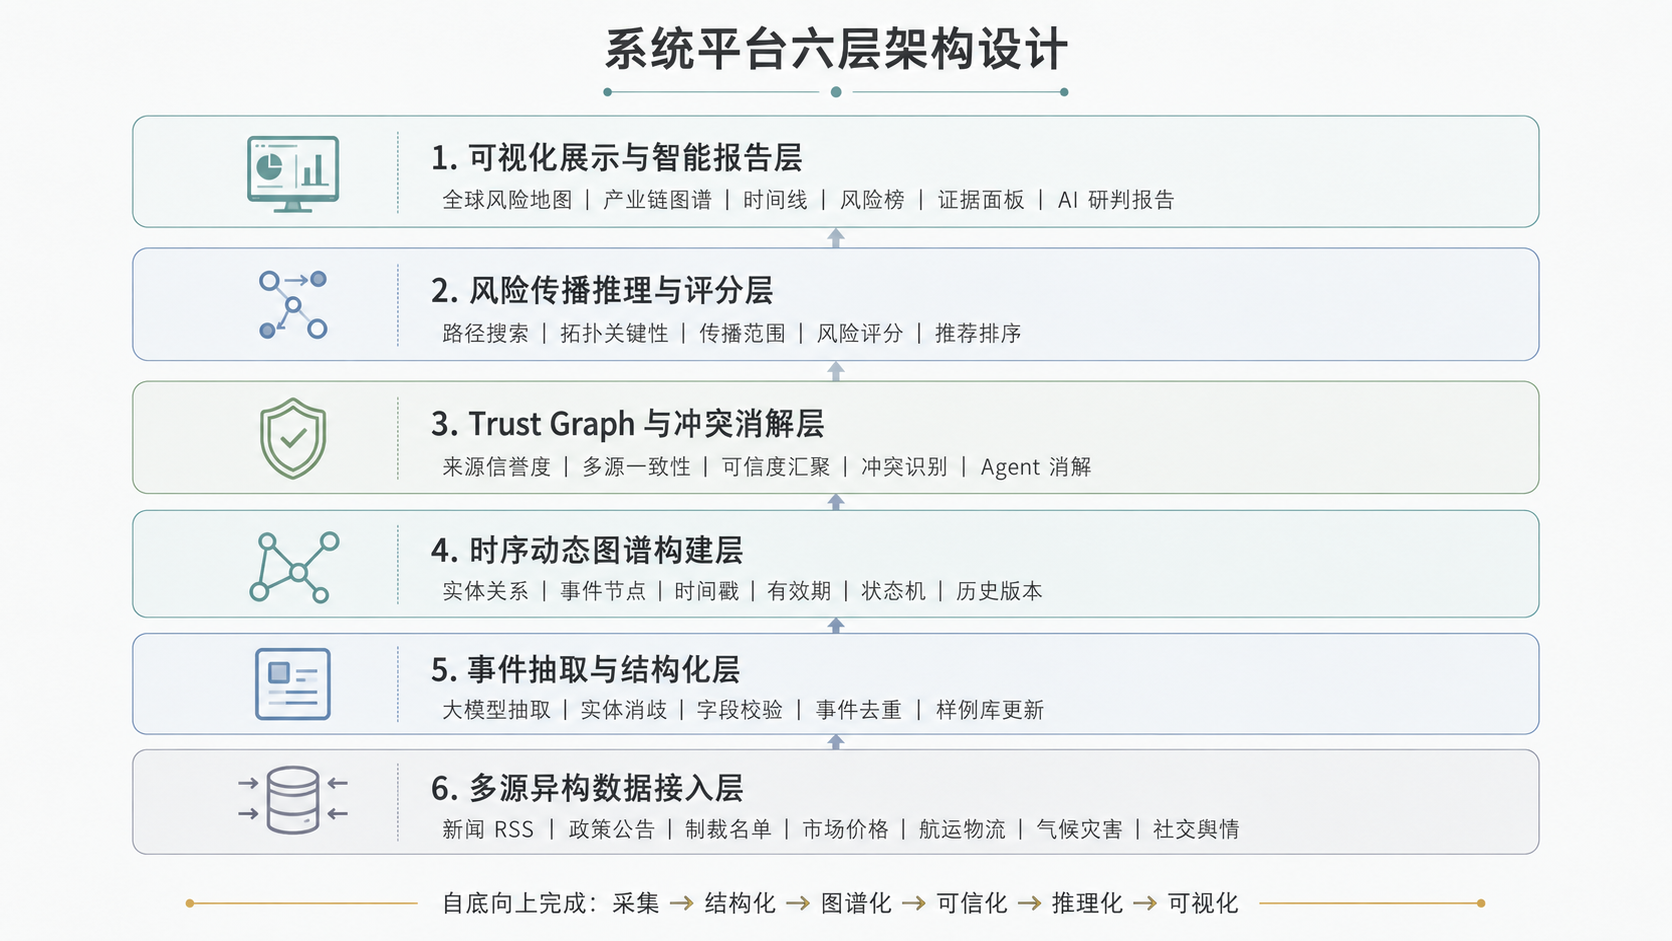
\includegraphics[width=0.95\linewidth]{图10.png}
\caption{系统平台六层架构设计}
\label{fig:platform-architecture}
\end{figure}

\paragraph{多源数据接入层。}该层负责采集和规范化不同来源数据。项目可复用现有开放情报工程中的 RSS、市场数据、制裁名单、灾害数据和社交媒体接入能力，并新增新能源产业链专业数据源。所有数据统一进入原始数据池，记录来源、时间、语言、链接和初始可信度。

\paragraph{事件抽取与结构化层。}该层负责将非结构化文本转化为结构化事件。系统采用大模型 Prompt、规则校验和实体词表结合的方式，输出标准事件 JSON，并进行去重、聚类和缺失字段补全。

\paragraph{时序动态图谱构建层。}该层是系统核心知识中枢。图谱节点包括国家、企业、材料、产业环节、物流通道、政策机构和风险事件；边包括供应、依赖、影响、运输、监管、制裁、证据支持和事件演化。每条边都带有时间和状态属性，避免静态图谱无法判断当前有效性的问题。

\paragraph{可信度评估与冲突消解层。}该层维护来源信誉度表、事件置信度、冲突状态和证据链。系统根据来源类型赋予基础分，再根据多源一致性和实体匹配质量进行修正。当事件存在冲突时，触发多智能体流程，输出 confirmed、conflicting、unverified、resolved 或 invalidated 等状态。

\paragraph{风险传播推理与评分层。}该层从事件节点出发，在产业链图谱中搜索影响路径，并综合事件严重度、节点关键性、置信度、传播范围和时间新鲜度计算风险分数。评分结果用于风险排序、预警触发和报告生成。

\paragraph{可视化展示与智能报告生成层。}该层面向用户提供交互式界面，包括全球风险地图、产业链动态图谱、事件时间线、风险节点排行榜、传播路径图、证据来源面板和 AI 研判报告。竞赛现场可通过典型案例演示系统如何从事件输入到报告输出。

\subsubsection{系统交互流程}

系统交互流程面向三类用户：企业供应链管理人员、金融投研人员和产业监管人员。不同用户的关注点不同，但底层交互都围绕“发现风险—理解风险—验证风险—推演风险—处置风险”展开。

\paragraph{用户主动查询流程。}用户在前端输入自然语言问题，如“智利锂矿罢工是否会影响碳酸锂价格”。系统解析意图后进行多路召回，展示相关事件卡片、证据来源、产业链路径和风险评分。用户可点击任一节点查看上下游关系、历史事件和相关报告。

\paragraph{系统主动预警流程。}系统定时采集多源数据，当新增事件匹配高关键性节点、来源置信度较高或短期内多源重复出现时，自动触发风险评分。如果评分超过阈值，系统生成预警卡片并推送到仪表盘。预警卡片包含风险等级、置信度、受影响节点和建议关注事项。

\paragraph{事件回溯流程。}用户可选择任一事件，查看其状态演化链。例如某事件从 rumor 变为 confirmed，再变为 active，最后 resolved。系统展示每次状态变化的证据来源、时间戳和原因，帮助用户理解风险判断如何形成。

\paragraph{报告生成流程。}用户点击“生成研判报告”后，系统将事件摘要、证据链、图谱路径、评分因子和历史状态作为上下文输入大模型。报告按固定结构输出，避免生成散乱文本。报告内容包括摘要、证据、影响路径、评分解释、潜在影响、应对建议和后续监控重点。

\begin{figure}[H]
\centering
\resizebox{\linewidth}{!}{
\begin{tikzpicture}[
    font=\footnotesize, % 节点主字体调整为 footnotesize 提升整体空间宽裕度
    % 统一采用 text width 替代 minimum width，强制规范物理边界
    actor/.style={draw=LineGray, rounded corners=2mm, thick, align=center, text width=1.4cm, minimum height=0.75cm, fill=SoftBlue},
    proc/.style={draw=LineGray, rounded corners=2mm, thick, align=center, text width=2.2cm, minimum height=0.75cm, fill=SoftOrange},
    core/.style={draw=DeepBlue, rounded corners=2mm, very thick, align=center, text width=2.2cm, minimum height=0.8cm, fill=Mint},
    arr/.style={-{Latex[length=1.8mm]}, thick, draw=LineGray}
]
% 第一行：采用非等距排布，按需分配横向空间
\node[actor] (user) {用户};
\node[proc, right=1.6cm of user] (front) {前端仪表盘}; % 间距拉宽，容纳“查询/筛选”
\node[proc, right=0.8cm of front] (api) {后端 API}; % 无文字，间距保持紧凑
\node[core, right=1.6cm of api] (kg) {动态图谱}; % 间距拉宽，容纳“检索证据”

% 第二行：严格复用第一行的物理间距参数，确保垂直方向上的节点完美对齐
\node[core, below=1.2cm of kg] (trust) {可信评估}; % 垂直间距拉宽，服务于左侧的闭环文字
\node[core, left=1.6cm of trust] (risk) {风险评分};
\node[core, left=0.8cm of risk] (llm) {LLM 报告};
\node[proc, left=1.6cm of llm] (view) {可视化结果};

% 正向流水线绘制，连线文字降级为 scriptsize
\draw[arr] (user) -- node[above, font=\scriptsize]{查询/筛选} (front);
\draw[arr] (front) -- (api);
\draw[arr] (api) -- node[above, font=\scriptsize]{检索证据} (kg);
\draw[arr] (kg) -- (trust);
\draw[arr] (trust) -- (risk);
\draw[arr] (risk) -- (llm);
\draw[arr] (llm) -- (view);

% 闭环反馈线段：文本必须换行 (\\) 且向右对齐 (align=right)，防止过度侵占左侧页面边距
\draw[arr] (view) -- node[left, align=right, font=\scriptsize]{图谱、路径\\与研判报告} (user);

\end{tikzpicture}
}
\caption{系统交互闭环流程}
\label{fig:interaction-flow}
\end{figure}

平台预期形成以下可展示模块。

\begin{itemize}
\item \term{全球风险地图：}按照事件地点展示政策、制裁、灾害、航运和市场风险，支持时间筛选和风险等级筛选。
\item \term{产业链动态图谱：}展示国家、材料、企业、环节和事件之间的关系，支持点击节点查看上下游影响路径。
\item \term{风险事件时间线：}按时间展示事件状态变化，突出风险升级、缓解和解决节点。
\item \term{风险节点排行榜：}根据节点关键性、事件数量、风险分数和传播范围排序，发现高风险材料、区域和企业。
\item \term{证据来源面板：}展示支持证据、冲突证据、来源类型、可信度和更新时间。
\item \term{AI 研判报告面板：}自动生成结构化行业报告，并提供风险分数解释和后续监控建议。
\end{itemize}

为了保证展示效果，系统将准备“实时模式”和“演示模式”。实时模式用于展示系统真实采集与更新能力；演示模式使用已验证的典型事件样例，保证现场网络不稳定时仍能完整演示风险发现、图谱推理、评分和报告生成流程。项目最终希望达到的效果是：评委输入一个近期或预设产业风险事件，系统能够在数秒至数十秒内生成受影响产业链图谱、风险传播路径、证据链、风险分数和智能研判报告，直观体现“AI + 图谱 + 产业风控”的融合价值。


% ====================== 3 实施方案 ======================
\section{实施方案}

本章围绕\projectname（以下简称\projectshort）给出完整实施方案。项目总体遵循“多源感知—事件抽取—时序建图—可信校验—风险传播—智能研判—可视化预警”的技术闭环，面向新能源锂电池产业链中政策突变、矿产供应扰动、航运阻塞、地缘冲突、价格异常、制裁合规、极端天气等黑天鹅风险场景，构建一个兼具行业知识、时间感知、可信度判断、图推理能力和大语言模型表达能力的垂直领域智能系统。

与普通新闻聚合、关键词告警或传统 RAG 问答系统不同，本项目不将大语言模型作为孤立的文本生成器，而是将其置于“时序可信动态图谱”的结构化推理框架之中。系统首先将跨源异构信息转化为标准化风险事件，再将事件挂接到新能源锂电池产业链图谱中，进一步通过时间状态机、来源可信度、图拓扑关键性、传播路径搜索和多 Agent 证据校验机制，对事件影响范围、风险等级、置信程度和应对建议进行综合计算，最终形成可解释、可追溯、可展示的产业链黑天鹅风险预警结果。

\subsection{技术可行性分析}

\subsubsection{数据采集与行业知识获取可行性}

新能源锂电池产业链具有天然适合知识图谱建模和风险事件结构化抽取的行业特征。一方面，该产业链覆盖上游矿产资源、中游电池材料与电芯制造、下游新能源汽车和储能应用，产业链条清晰、实体类型稳定、上下游依赖关系明确，适合抽象为“国家—资源—材料—企业—物流—市场—政策”的多层异构图结构。另一方面，锂、镍、钴、石墨、碳酸锂、氢氧化锂、硫酸镍等关键材料具有高度国际化供应特征，其风险信息广泛分布于新闻报道、政府公告、企业公告、金融资讯、航运数据、气候灾害数据和社交媒体之中，具备持续采集、交叉验证和事件化建模的数据基础。

本项目从零搭建面向新能源锂电池产业链的多源风险数据采集体系。系统不依赖单一数据源，而是面向产业链黑天鹅风险场景构建多通道数据入口，包括全球新闻、政策公告、制裁清单、行业资讯、市场价格、航运物流、气候灾害和舆情信息等。不同数据源在信息粒度、可信程度、更新频率和风险敏感性上各有差异：官方公告更适合确认政策与监管事件，主流媒体更适合识别重大突发事件，行业媒体更适合补充产业链细节，市场价格数据可用于验证供需扰动，社交舆情则可用于捕捉早期异常信号。通过多源协同，系统能够形成覆盖“事实确认—趋势感知—风险预警—证据追溯”的完整数据闭环。

在行业知识构建方面，项目将自主整理新能源锂电池产业链基础知识库，覆盖国家、地区、矿产资源、材料品类、企业主体、产业环节、运输通道、政策类型、风险事件类型等核心对象。初始知识库不追求无限规模，而是优先覆盖高风险、高频出现和高解释价值的关键节点。例如，上游重点覆盖智利、阿根廷、澳大利亚、印尼、刚果金等关键资源国；材料侧重点覆盖锂、镍、钴、石墨、碳酸锂、氢氧化锂、硫酸镍等关键材料；企业侧重点覆盖电池制造商、矿产企业、材料企业、整车企业和储能企业；物流侧重点覆盖红海、马六甲海峡、苏伊士运河、主要港口和跨境运输通道。通过这种“重点优先、逐步扩展”的方式，项目可以在有限时间内形成高质量、可解释、可展示的产业链风险图谱。

系统规划如下自研工程目录，以体现从数据采集到风险预警的完整自主实现链路：
\begin{itemize}
    \item 多源数据接入模块：\path{src/data_ingestion/}
    \item 新闻与公告解析模块：\path{src/document_parser/}
    \item 事件抽取与字段校验模块：\path{src/event_extraction/}
    \item 产业链知识图谱构建模块：\path{src/knowledge_graph/}
    \item 时序图谱状态管理模块：\path{src/temporal_graph/}
    \item 来源可信度与冲突消解模块：\path{src/trust_graph/}
    \item 风险传播路径推理模块：\path{src/risk_reasoning/}
    \item 综合风险评分模块：\path{src/risk_scoring/}
    \item 大语言模型研判报告模块：\path{src/llm_report/}
    \item 可视化预警前端模块：\path{src/dashboard/}
    \item 样例事件与演示数据集：\path{data/demo_events/}
    \item 产业链图谱种子数据：\path{data/kg_seed/}
    \item 来源信誉规则配置：\path{config/source_trust_rules.json}
    \item 风险类型与事件状态配置：\path{config/risk_event_schema.json}
\end{itemize}

因此，本项目的数据采集与行业知识获取具有较强可行性。其关键不在于单纯堆叠数据规模，而在于将多源开放信息转化为可计算、可验证、可追溯的产业链风险事件，并进一步映射到时序可信动态图谱中，为后续风险传播推理和智能研判提供结构化基础。

\subsubsection{核心算法可行性}

本项目所需算法模块可以采用“规则模型 + 图算法 + 大语言模型 + 可解释评分”的组合式路线实现。该路线不依赖大规模模型训练，也不要求从零训练专用基础模型，因而具备较高的实现确定性和比赛可交付性。

首先，在事件抽取阶段，可使用通用大语言模型或轻量级信息抽取模型，将新闻文本、公告文本和舆情文本转化为统一事件结构。对于比赛演示，可同时保留离线样例数据集和在线实时数据流，避免现场网络波动或外部接口不稳定影响展示效果。

其次，在图谱构建阶段，产业链上下游关系具有相对稳定的先验结构，可以通过人工整理、公开资料归纳和样例库增强构建初始图谱。图谱中的事件节点、实体节点和关系边均可加入时间属性、置信度属性和状态属性，从而支持按时间回溯、按状态过滤和按置信度排序。

再次，在风险传播阶段，可以采用可解释图搜索和图拓扑算法实现。例如，系统可基于 BFS、加权最短路径、路径衰减传播、PageRank、Degree Centrality、Betweenness Centrality 和 Community Detection 等方法计算风险影响路径和节点关键性。由于这些方法成熟稳定、计算开销可控，非常适合作为比赛系统中的核心推理引擎。

最后，在报告生成阶段，大语言模型并不直接“拍脑袋”判断风险，而是接收结构化证据包作为输入，包括事件摘要、时间状态、证据来源、置信度分数、影响路径、关键节点、传播范围和风险评分。通过这种方式，大语言模型主要负责自然语言表达、逻辑组织和决策建议生成，而核心判断依据由图谱和评分模型提供，从而降低幻觉风险，提高结果可解释性。

\subsubsection{算力与硬件资源可行性}

项目整体计算负载可拆分为离线构建与在线推理两部分。离线部分主要包括产业链图谱初始化、历史事件样例整理、实体别名表构建、来源信誉表维护、拓扑指标批量计算等任务；在线部分主要包括实时数据采集、事件抽取、图谱写入、可信度计算、传播路径搜索、风险评分和报告生成。

在比赛阶段，本项目可以采用轻量部署方案：
\begin{itemize}
    \item 后端服务使用 Node.js/Express 承载数据接口、缓存、推理和报告生成流程；
    \item 图谱数据在 MVP 阶段可使用 JSON 文件或轻量本地存储维护，后续扩展为 Neo4j；
    \item 原文向量检索可在增强版中接入 pgvector、FAISS 或其他向量数据库；
    \item 大语言模型调用可采用云端 API、本地 Ollama 模型或 OpenRouter 等统一封装方式；
    \item 前端使用单页 Dashboard 展示全球风险地图、事件时间线、产业链图谱、风险榜单和 AI 报告。
\end{itemize}

对于参赛演示而言，该架构能够在普通开发机或轻量云服务器上稳定运行。由于高开销模型推理环节可以通过缓存机制、样例事件预生成和增量更新策略降低实时压力，系统具备良好的展示稳定性和工程可控性。

\subsubsection{自主研发路线与工程扩展可行性}

本项目的工程实现强调自主可控和渐进式增强。系统并不将已有通用问答框架作为核心依赖，而是从新能源锂电池产业链风险任务本身出发，重新设计数据结构、事件 Schema、图谱模型、可信度计算规则、风险评分公式和前端展示逻辑。这样的设计能够更好地服务比赛中的技术表达：项目不是“把新闻接入大模型”，而是构建一个面向产业链风险认知的智能推理系统。

系统自研路线分为三个层次。

第一层是基础工程层，目标是保证系统能够稳定运行。该层包括数据采集、数据清洗、接口服务、缓存管理、日志记录、配置管理和前端页面。基础工程层不追求复杂算法，而是确保系统具备完整的数据流和稳定的演示能力。

第二层是核心智能层，目标是体现项目技术深度。该层包括事件抽取、实体对齐、时序图谱构建、来源可信度建模、多源冲突消解、图传播搜索、节点关键性计算和风险评分。这些模块直接决定系统是否区别于普通 RAG、普通新闻摘要和普通可视化平台。

第三层是展示决策层，目标是提升系统应用价值和比赛呈现效果。该层包括全球风险地图、产业链图谱、风险事件时间线、影响路径图、风险节点榜单、证据链面板和 AI 研判报告。该层不仅展示结果，还展示“为什么得出该结果”，使系统具备可解释决策支持能力。

系统扩展性主要体现在以下方面：
\begin{itemize}
    \item \term{数据源可扩展}：新增数据源只需适配统一文档对象，无需修改核心推理逻辑；
    \item \term{事件类型可扩展}：新增风险类型只需更新事件 Schema 和评分规则；
    \item \term{图谱节点可扩展}：新增企业、材料、地区或物流通道可直接写入图谱种子库；
    \item \term{模型可替换}：事件抽取和报告生成模块可灵活切换不同大语言模型；
    \item \term{存储可升级}：原型阶段可使用本地文件和轻量数据库，后续可升级为 Neo4j、pgvector 等专业存储；
    \item \term{算法可增强}：初期使用规则与图搜索，后续可接入图神经网络、时间序列预测和多 Agent 强化协同。
\end{itemize}

因此，本项目既能在短周期内形成稳定可演示原型，又具备继续扩展为产业级风险监测平台的工程潜力。

\subsubsection{系统工程可行性}

本项目采用完全模块化的自主研发路线，从底层数据接入到上层可视化预警均围绕新能源锂电池产业链风险场景进行定制化设计。系统整体遵循“低耦合、高内聚、可替换、可演示、可扩展”的工程原则，将复杂系统拆解为若干相对独立的功能模块，包括数据接入模块、文本解析模块、事件抽取模块、图谱构建模块、可信度评估模块、风险推理模块、报告生成模块和前端可视化模块。各模块之间通过统一事件 Schema 和标准化风险对象进行通信，既便于团队并行开发，也便于后续调试、替换和扩展。

从工程实现角度看，系统可采用前后端分离架构。后端负责数据采集、事件抽取、图谱维护、风险评分和报告生成；前端负责全球风险地图、产业链图谱、风险时间线、节点风险榜单、证据链面板和 AI 研判报告展示。后端服务可使用 Python FastAPI、Node.js 或其他轻量 Web 框架实现，图谱存储在原型阶段可采用 JSON、SQLite 或本地轻量图结构，增强阶段可扩展为 Neo4j；向量检索在原型阶段可使用本地 Embedding 索引，后续可扩展为 FAISS、pgvector 或其他向量数据库。该路线既保证原型系统快速落地，又为后续工程升级保留足够空间。

系统数据流采用统一标准对象传递。原始数据首先被归一化为文档对象：
\begin{equation}
d_i=(\text{id},\text{source},\text{title},\text{content},\text{url},\text{published\_at},\text{metadata}),
\end{equation}
随后经事件抽取模块转化为风险事件对象：
\begin{equation}
e_i=(\text{type},\text{time},\text{location},\text{entities},\text{affected\_nodes},\text{severity},\text{status},\text{evidence}),
\end{equation}
再写入时序可信动态图谱：
\begin{equation}
\mathcal{G}_{\tau}=(\mathcal{V},\mathcal{E}_{\tau},\mathcal{R},\mathcal{C}_{\tau},\mathcal{S}_{\tau}),
\end{equation}
最终输出风险报告对象：
\begin{equation}
r_i=(\text{risk\_score},\text{risk\_level},\text{confidence},\text{paths},\text{key\_nodes},\text{evidence},\text{advice}).
\end{equation}

\begin{figure}[H]
\centering
\resizebox{\linewidth}{!}{
\begin{tikzpicture}[
    font=\small,
    node distance=0.75cm,
    % 修复 1：将 minimum width 替换为 text width，强制内部长文本换行，维持严格的边界尺寸
    layer/.style={rectangle, rounded corners=3pt, draw=DeepBlue, thick, fill=SoftBlue, text width=4.8cm, minimum height=0.75cm, align=center},
    core/.style={rectangle, rounded corners=3pt, draw=TechBlue, thick, fill=Mint, text width=4.8cm, minimum height=0.75cm, align=center},
    % 修复 2：彻底避开保留字，重命名为 outbox
    outbox/.style={rectangle, rounded corners=3pt, draw=LineGray, thick, fill=SoftOrange, text width=4.8cm, minimum height=0.75cm, align=center},
    % 优化 1：为箭头连线增加 rounded corners，使所有的 90 度直角折线拥有平滑美观的过渡
    arrow/.style={-{Latex[length=2mm]}, thick, draw=LineGray, rounded corners=2mm}
]

% 主干数据流 (中列)
\node[layer] (raw) {原始多源数据\\新闻、公告、制裁、价格、航运、灾害、舆情};
\node[layer, below=of raw] (doc) {标准文档对象\\清洗、去重、时间归一、来源注册};
\node[layer, below=of doc] (event) {结构化风险事件\\实体、类型、时间、地点、严重度、证据};
\node[core, below=of event] (graph) {时序可信动态图谱\\状态机、有效期、置信度、证据链};
\node[core, below=of graph] (score) {风险传播推理与评分\\路径搜索、关键节点、传播范围、风险等级};
\node[outbox, below=of score] (ui) {可视化预警与智能研判\\地图、时间线、图谱、榜单、报告};

% 中列顺次相连
\draw[arrow] (raw) -- (doc);
\draw[arrow] (doc) -- (event);
\draw[arrow] (event) -- (graph);
\draw[arrow] (graph) -- (score);
\draw[arrow] (score) -- (ui);

% 辅助处理模块 (右侧：可信度)
\node[rectangle, rounded corners=3pt, draw=TechBlue, fill=SoftPurple, align=center, text width=3.2cm, minimum height=0.7cm, right=1.2cm of graph] (trust) {可信度引擎\\来源信誉\\一致性\\冲突消解};

\draw[arrow] (trust.west) -- (graph.east);
% 优化 2：摒弃斜线，使用 |- (先垂直向下，再水平向左) 实现完美的直角扇入
\draw[arrow] (trust.south) |- (score.east);

% 辅助处理模块 (左侧：大模型)
\node[rectangle, rounded corners=3pt, draw=DeepBlue, fill=SoftRed, align=center, text width=3.2cm, minimum height=0.7cm, left=1.2cm of score] (llm) {大模型智能体\\事件抽取\\证据归纳\\报告生成};

% 优化 3：摒弃容易发生碰撞的手动偏移量 (++)，使用 -| (先向左水平探出，再垂直向下)
\draw[arrow] (event.west) -| (llm.north);
\draw[arrow] (llm.east) -- (score.west);
% 再次利用 |- 实现向下的回流
\draw[arrow] (llm.south) |- (ui.west);

\end{tikzpicture}
}
\caption{\projectshort 自研系统工程闭环}
\label{fig:self-built-engineering-loop}
\end{figure}

这种对象化设计能够显著降低系统复杂度，使各模块职责清晰、输入输出明确。事件抽取模块只需保证输出字段合法；图谱模块只需保证事件能够正确挂接到实体和关系上；可信度模块只需更新置信度与冲突状态；风险推理模块只需读取图谱并输出路径、分数和解释；前端模块只需消费标准化接口即可完成展示。

如图 \ref{fig:self-built-engineering-loop} 所示，系统从原始开放数据出发，经过文档对象化、事件结构化、图谱动态化、可信度校验、传播推理和可视化预警，形成完整的端到端自研闭环。该工程路线能够充分体现项目并非简单调用大模型或包装现有工具，而是围绕产业链黑天鹅风险任务构建了一套具有垂直领域特征的智能系统。

\subsubsection{风险控制与比赛演示可行性}

为保证比赛交付效果，本项目采用“实时模式 + 离线样例模式”双轨运行机制。实时模式用于展示系统对最新新闻、政策和市场信息的响应能力；离线样例模式用于保证在网络接口、第三方服务或模型 API 不稳定时仍能完整演示系统核心功能。样例库重点覆盖五类高辨识度场景：
\begin{itemize}
    \item 印尼镍矿出口政策变化导致三元正极材料供应波动；
    \item 智利锂矿罢工导致碳酸锂价格预期上行；
    \item 红海航运中断影响欧洲电池供应链运输；
    \item 刚果金钴矿政策变化影响钴资源供应稳定性；
    \item 欧盟电池法案更新引发出口合规和碳足迹披露风险。
\end{itemize}

通过上述策略，项目既能展示真实系统能力，又能避免比赛现场偶发因素造成演示失败。系统最终可以形成可运行 Web Demo、技术报告、答辩 PPT、演示视频和典型案例库，具备完整参赛交付形态。

\subsection{技术细节}

\subsubsection{总体技术架构}

本项目总体架构划分为六层：多源数据接入层、事件抽取与结构化层、时序动态图谱构建层、可信度评估与冲突消解层、风险传播推理与评分层、可视化展示与智能报告生成层。六层之间通过标准事件对象、图谱节点对象、证据对象和风险报告对象进行连接。

\begin{figure}[H]
\centering
\resizebox{\linewidth}{!}{
\begin{tikzpicture}[
    font=\scriptsize,
    box/.style={rectangle, rounded corners=3pt, draw=DeepBlue, thick, fill=SoftBlue, align=center, minimum width=3.0cm, minimum height=0.75cm},
    core/.style={rectangle, rounded corners=3pt, draw=TechBlue, thick, fill=Mint, align=center, minimum width=3.0cm, minimum height=0.75cm},
    agent/.style={rectangle, rounded corners=3pt, draw=LineGray, thick, fill=SoftPurple, align=center, minimum width=2.8cm, minimum height=0.7cm},
    arrow/.style={-{Latex[length=2mm]}, thick, draw=LineGray}
]
\node[box] (rss) {新闻/RSS\\GDELT/行业媒体};
\node[box, right=0.55cm of rss] (policy) {政策/制裁\\政府公告/OFAC};
\node[box, right=0.55cm of policy] (market) {市场/航运/灾害\\价格/船舶/天气};
\node[box, right=0.55cm of market] (social) {社交舆情\\论坛/社媒/传闻};

\node[core, below=0.9cm of policy, xshift=1.75cm] (extract) {事件抽取与字段校验\\Event Schema + LLM Parser};
\node[core, below=0.75cm of extract] (tkg) {时序可信动态图谱\\Temporal KG + Trust Graph};
\node[core, below=0.75cm of tkg] (reason) {风险传播推理\\Graph Reasoner + Risk Scorer};
\node[box, below=0.75cm of reason] (vis) {前端可视化\\地图、图谱、时间线、榜单、报告};

\node[agent, left=0.75cm of tkg] (agent1) {冲突消解 Agent\\多源证据辩论};
\node[agent, right=0.75cm of tkg] (agent2) {报告生成 Agent\\证据链转研判};

\draw[arrow] (rss.south) |- (extract.west);
\draw[arrow] (policy.south) -- (extract.north);
\draw[arrow] (market.south) |- (extract.east);
\draw[arrow] (social.south) |- (extract.east);
\draw[arrow] (extract) -- (tkg);
\draw[arrow] (tkg) -- (reason);
\draw[arrow] (reason) -- (vis);
\draw[arrow] (agent1) -- (tkg);
\draw[arrow] (tkg) -- (agent2);
\draw[arrow] (agent2) |- (vis.east);
\end{tikzpicture}
}
\caption{\projectshort 总体技术架构}
\label{fig:overall-arch}
\end{figure}

该架构体现三个关键特点。第一，系统从数据入口开始即面向风险事件建模，而非简单文本存储。第二，系统将时间状态、来源可信度和图拓扑关键性作为一等公民写入图谱，使风险推理具备结构依据。第三，系统将 LLM 放置在可控边界内，主要承担信息抽取、证据归纳和报告生成任务，从而避免完全依赖黑箱生成。

\subsubsection{系统核心模块实现与代码证据}

\begin{figure}[H]
\centering
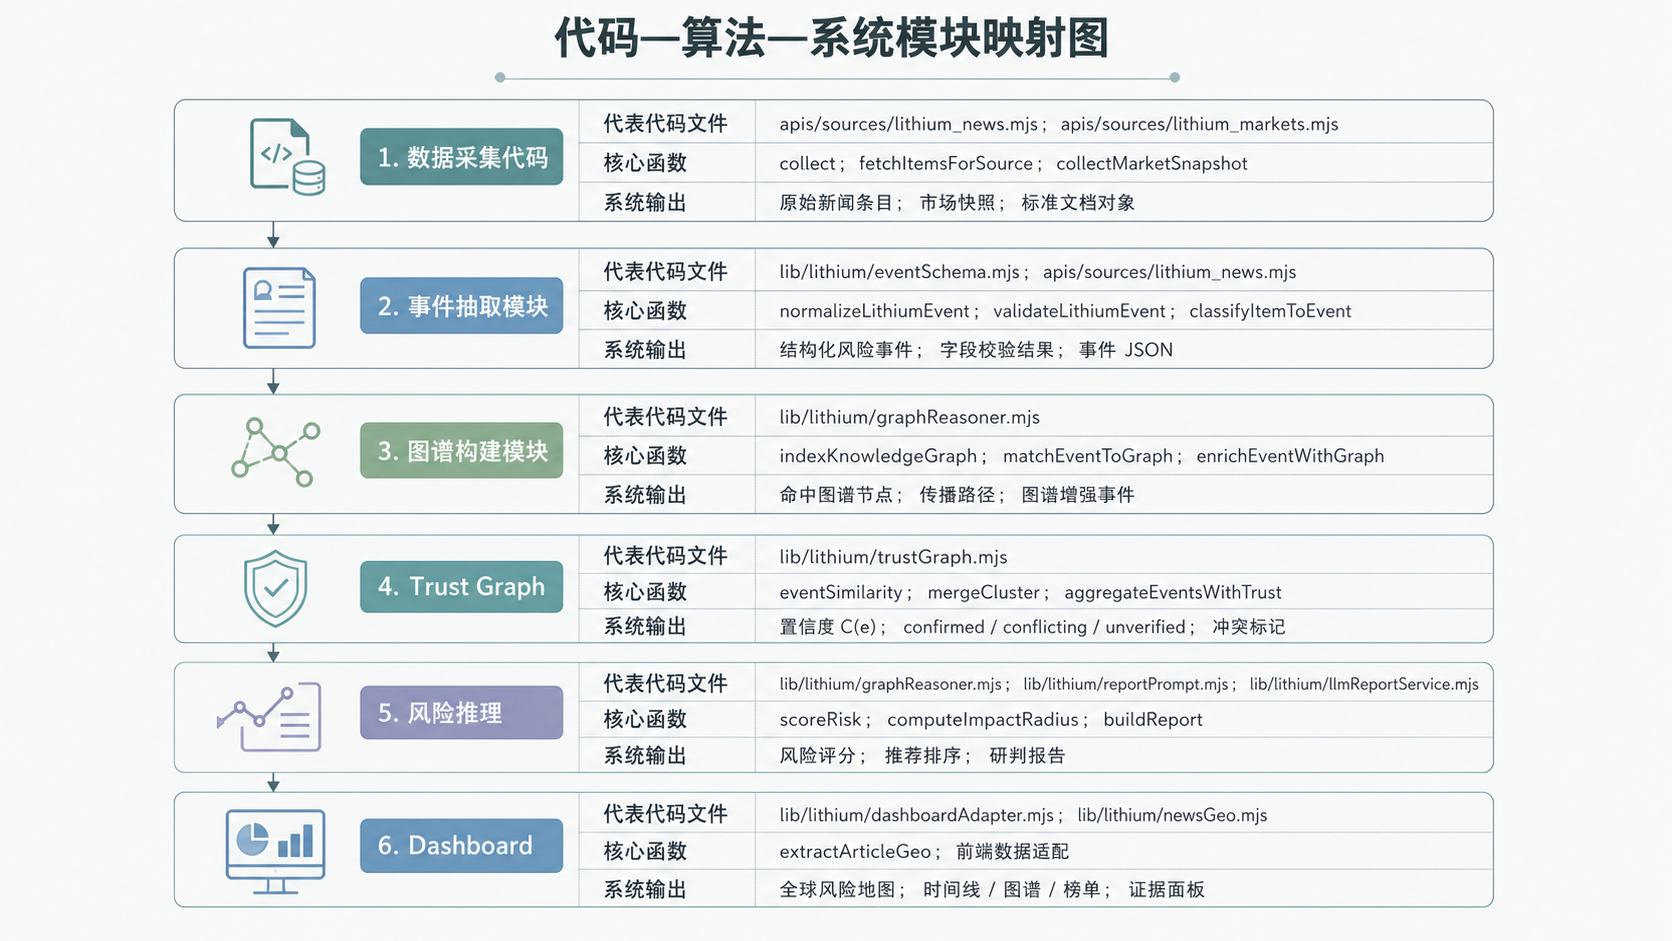
\includegraphics[width=0.95\linewidth]{新增，放在3.2.2 系统核心模块实现与代码证据开头.png}
\caption{系统核心模块架构总览}
\label{fig:core-modules}
\end{figure}

为避免系统停留在概念设计层面，本项目已经围绕新能源锂电池产业链风险推理任务完成了若干核心模块的工程实现。当前原型系统不是简单调用大语言模型生成文本，而是形成了从多源信息接入、风险事件标准化、产业链图谱匹配、传播路径搜索、可信度聚合、风险评分、市场数据监测到智能研判报告生成的完整闭环。

核心实现文件包括：
\begin{itemize}
    \item 风险事件标准化与字段校验：\path{lib/lithium/eventSchema.mjs}
    \item 产业链图谱匹配与风险传播推理：\path{lib/lithium/graphReasoner.mjs}
    \item Trust Graph 可信度聚合与冲突消解：\path{lib/lithium/trustGraph.mjs}
    \item 多源新闻采集与事件抽取：\path{apis/sources/lithium_news.mjs}
    \item 市场价格与金融代理指标监测：\path{apis/sources/lithium_markets.mjs}
    \item 地理位置抽取与地图定位增强：\path{lib/lithium/newsGeo.mjs}
    \item 本地增量事件库与缓存管理：\path{lib/lithium/localStore.mjs}
    \item 结构化研判报告 Prompt 构造：\path{lib/lithium/reportPrompt.mjs}
    \item LLM 研判报告生成与缓存：\path{lib/lithium/llmReportService.mjs}
    \item 前端仪表盘数据适配：\path{lib/lithium/dashboardAdapter.mjs}
\end{itemize}

这些模块共同构成了 \projectshort 的工程骨架。其中，事件 Schema 保证了系统输入输出的一致性；图谱推理模块负责将风险事件映射到产业链结构；Trust Graph 模块负责多源证据聚合和冲突标记；报告模块则将结构化证据链转化为可解释的行业研判文本。

\paragraph{1. 风险事件标准化与字段校验实现}

系统首先将不同来源的新闻、公告、价格、航运或灾害信息统一归一化为标准风险事件对象。该模块定义了事件类型、生命周期状态、验证状态、产业链阶段、关键材料和风险等级，并通过标准化函数将原始输入转换为可计算、可校验、可写入图谱的数据对象。

\begin{lstlisting}[style=projectcode,caption={风险事件标准化与 Schema 校验核心实现}]
export const EVENT_TYPES = [
  'policy_change', 'sanction', 'supply_disruption',
  'logistics_disruption', 'natural_disaster', 'price_spike',
  'labor_strike', 'geopolitical_conflict',
  'environment_regulation', 'corporate_action',
  'production_change', 'demand_shift',
  'technology_change', 'rumor', 'other',
];

export const LIFECYCLE_STATUS = [
  'rumor', 'confirmed', 'escalating', 'active',
  'mitigating', 'resolved', 'invalidated',
];

export const VERIFICATION_STATUS = [
  'confirmed', 'conflicting', 'unverified',
  'resolved', 'invalidated',
];

export function riskLevelFromScore(score) {
  const s = Number(score);
  if (!Number.isFinite(s)) return 'low';
  if (s <= 30) return 'low';
  if (s <= 60) return 'medium';
  if (s <= 80) return 'high';
  return 'critical';
}

export function normalizeLithiumEvent(input = {}) {
  const source = input.source ?? {};
  const severity = clamp01(input.severity, 0.3);
  const confidence = clamp01(
    input.confidence ?? source.base_trust,
    clamp01(source.base_trust, 0.5)
  );

  const score = input.risk?.score ?? input.risk_score ?? Math.round(100 * (
    severity * 0.35 + confidence * 0.20
  ));

  return {
    schema_version: SCHEMA_VERSION,
    event_id: input.event_id ?? makeEventId({
      sourceId: source.source_id,
      url: source.url,
      title: input.event_name ?? input.title,
      time: input.time ?? input.event_time ?? input.published_at,
    }),

    event_type: input.event_type ?? 'other',
    event_name: String(input.event_name ?? input.title ?? '').trim(),
    summary: String(input.summary ?? input.description ?? '').trim(),

    time: {
      published_at: input.time?.published_at ?? input.published_at ?? null,
      event_time: input.time?.event_time ?? input.event_time ?? null,
      valid_from: input.time?.valid_from ?? input.valid_from ?? null,
      valid_to: input.time?.valid_to ?? input.valid_to ?? null,
      extracted_at: input.time?.extracted_at ?? new Date().toISOString(),
    },

    entities: asArray(input.entities).map(normalizeEntity),
    materials: asArray(input.materials),
    supply_chain_stages: asArray(input.supply_chain_stages),
    affected_nodes: asArray(input.affected_nodes),

    lifecycle_status: input.lifecycle_status ?? input.status ?? 'active',
    verification_status: input.verification_status ?? 'unverified',
    severity,
    confidence,

    source: {
      source_id: source.source_id ?? null,
      name: source.name ?? null,
      domain_bucket: source.domain_bucket ?? source.source_type ?? null,
      url: source.url ?? null,
      base_trust: clamp01(source.base_trust, 0.5),
    },

    evidence: asArray(input.evidence),
    graph: {
      matched_nodes: asArray(input.graph?.matched_nodes),
      propagation_paths: asArray(input.graph?.propagation_paths),
    },

    risk: {
      score,
      risk_level: input.risk?.risk_level ?? riskLevelFromScore(score),
      impact_radius: input.risk?.impact_radius ?? null,
      rationale: input.risk?.rationale ?? null,
    },

    raw: input.raw ?? null,
  };
}

export function validateLithiumEvent(input = {}) {
  const event = normalizeLithiumEvent(input);
  const errors = [];

  if (!event.event_name) errors.push('event_name is required');
  if (!EVENT_TYPES.includes(event.event_type)) errors.push('invalid event_type');
  if (!LIFECYCLE_STATUS.includes(event.lifecycle_status)) errors.push('invalid lifecycle_status');
  if (!VERIFICATION_STATUS.includes(event.verification_status)) errors.push('invalid verification_status');
  if (!event.source?.source_id) errors.push('source.source_id is required');
  if (!event.source?.name) errors.push('source.name is required');
  if (event.evidence.length === 0) errors.push('at least one evidence item is required');

  return { ok: errors.length === 0, errors, event };
}
\end{lstlisting}

上述实现说明系统已经具备规范化事件协议，而不是仅依赖自由文本摘要。所有风险事件进入后续图谱推理和报告生成前，都必须通过统一事件 Schema 进行归一化和合法性校验。

\paragraph{2. 多源信息到风险事件的规则抽取实现}

在多源数据接入阶段，系统通过关键词规则、来源标签、事件类型映射和材料识别规则，将新闻、公告、灾害或市场信息初步转化为风险事件。该实现能够支持 RSS、HTML 链接扫描、社交平台 JSON、地震灾害 GeoJSON 等多种输入格式，并将其映射为统一事件对象。

\begin{lstlisting}[style=projectcode,caption={多源新闻条目到风险事件的抽取与映射}]
const MATERIAL_KEYWORDS = {
  lithium: ['lithium', 'li-ion', 'lithium carbonate'],
  nickel: ['nickel', 'nickel sulfate'],
  cobalt: ['cobalt'],
  graphite: ['graphite', 'anode'],
  ternary_cathode: ['ncm', 'nca', 'ternary', 'cathode'],
  lithium_iron_phosphate: ['lfp', 'lithium iron phosphate'],
};

const EVENT_RULES = [
  ['policy_change', ['policy', 'regulation', 'tariff', 'export control', 'export restriction']],
  ['sanction', ['sanction', 'blacklist', 'entity list']],
  ['supply_disruption', ['shortage', 'disruption', 'shutdown', 'force majeure']],
  ['logistics_disruption', ['shipping', 'port', 'red sea', 'suez', 'malacca']],
  ['natural_disaster', ['earthquake', 'flood', 'wildfire', 'storm', 'drought']],
  ['price_spike', ['price spike', 'surge', 'futures', 'spot price']],
  ['labor_strike', ['strike', 'protest', 'union']],
  ['geopolitical_conflict', ['war', 'conflict', 'tension', 'attack']],
];

function inferMaterials(text, source = {}) {
  const out = [];
  const combined = `${text}\n${asArray(source.coverage_tags).join(' ')}`;
  for (const [material, keywords] of Object.entries(MATERIAL_KEYWORDS)) {
    if (includesAny(combined, keywords)) out.push(material);
  }
  return [...new Set(out)];
}

function inferEventType(text, source = {}) {
  if (source.adapter === 'usgs_earthquake_geojson') return 'natural_disaster';
  for (const [type, keywords] of EVENT_RULES) {
    if (includesAny(text, keywords)) return type;
  }
  return 'other';
}

function inferAffectedNodes(materials, stages) {
  const nodes = new Set(materials);

  if (materials.includes('lithium')) {
    nodes.add('lithium_carbonate');
    nodes.add('lithium_hydroxide');
    nodes.add('cathode');
    nodes.add('battery_cell');
  }

  if (materials.includes('nickel')) {
    nodes.add('nickel_sulfate');
    nodes.add('ternary_cathode');
    nodes.add('battery_cell');
  }

  if (materials.includes('cobalt')) {
    nodes.add('ternary_cathode');
    nodes.add('battery_cell');
  }

  if (materials.includes('graphite')) {
    nodes.add('anode');
    nodes.add('battery_cell');
  }

  for (const stage of stages) nodes.add(stage);
  if (!nodes.size) {
    nodes.add('battery_cell');
    nodes.add('ev');
  }

  return [...nodes];
}

function classifyItemToEvent(item, source) {
  const text = `${item.title}\n${item.summary}`;
  const eventType = inferEventType(text, source);
  const materials = inferMaterials(text, source);
  const stages = inferStages(text, materials, eventType, source);
  const affectedNodes = inferAffectedNodes(materials, stages);

  const candidate = {
    event_type: eventType,
    event_name: item.title,
    summary: item.summary,
    published_at: item.published_at,
    entities: materials.map(m => ({ name: m, type: 'material' })),
    materials,
    supply_chain_stages: stages,
    affected_nodes: affectedNodes,
    lifecycle_status: 'active',
    verification_status: 'unverified',
    severity: severityFromType(eventType, materials, source),
    confidence: Math.max(0.2, Math.min(1, Number(source.base_trust ?? 0.5))),
    source,
    evidence: [{
      title: item.title,
      url: item.url || source.url,
      published_at: item.published_at ?? null,
      snippet: item.summary || source.description || '',
      source_id: source.source_id,
    }],
    raw: item,
  };

  const validated = validateLithiumEvent(candidate);
  return validated.ok ? validated.event : {
    ...validated.event,
    validation_errors: validated.errors,
  };
}
\end{lstlisting}

该模块体现了系统对“原始文本—结构化风险事件”的自动转换能力。即使不依赖大模型，系统也能够通过可解释规则完成初步事件识别、材料识别、产业链节点映射和风险严重度初始化。

\paragraph{3. 产业链知识图谱匹配与传播路径搜索实现}

系统将标准化风险事件映射到新能源锂电池产业链知识图谱中，并从命中节点出发搜索上下游传播路径。该模块已经实现实体别名索引、国家/物流节点提示匹配、图遍历、传播路径标注、影响半径计算和节点关键性计算。

\begin{lstlisting}[style=projectcode,caption={事件到产业链图谱的匹配与传播路径搜索}]
export function indexKnowledgeGraph(kg) {
  const nodeById = new Map();
  const aliasToId = new Map();
  const outgoing = new Map();
  const incoming = new Map();

  for (const node of kg.nodes ?? []) {
    nodeById.set(node.id, node);
    const aliases = new Set([node.id, node.label, ...(node.aliases ?? [])]);

    for (const alias of aliases) {
      const normalized = normalizeToken(alias);
      const compact = compactToken(alias);
      if (normalized) aliasToId.set(normalized, node.id);
      if (compact) aliasToId.set(compact, node.id);
    }
  }

  for (const edge of kg.edges ?? []) {
    if (!outgoing.has(edge.source)) outgoing.set(edge.source, []);
    if (!incoming.has(edge.target)) incoming.set(edge.target, []);
    outgoing.get(edge.source).push(edge);
    incoming.get(edge.target).push(edge);
  }

  return { ...kg, nodeById, aliasToId, outgoing, incoming };
}

export function matchEventToGraph(event, kg) {
  const e = normalizeLithiumEvent(event);
  const matches = new Set();

  for (const x of e.affected_nodes ?? []) addAliasMatch(matches, kg, x);
  for (const x of e.materials ?? []) addAliasMatch(matches, kg, x);
  for (const x of e.supply_chain_stages ?? []) addAliasMatch(matches, kg, x);
  for (const ent of e.entities ?? []) addAliasMatch(matches, kg, ent.name);

  const textNorm = normalizeToken(eventSearchText(e));

  const logisticsHints = [
    ['logistics_red_sea', ['red sea']],
    ['logistics_suez', ['suez', 'suez canal']],
    ['logistics_malacca', ['malacca', 'malacca strait']],
  ];

  for (const [nodeId, hints] of logisticsHints) {
    if (hints.some(h => textNorm.includes(normalizeToken(h)))) {
      matches.add(nodeId);
    }
  }

  return [...matches].filter(id => kg.nodeById.has(id));
}

export function findPropagationPaths(
  kg,
  startIds,
  { maxDepth = 5, maxPathsPerStart = 8 } = {}
) {
  const paths = [];
  const seenPaths = new Set();

  function dfs(nodeId, path, depth) {
    if (depth >= maxDepth) return;

    const edges = kg.outgoing.get(nodeId) ?? [];
    for (const edge of edges) {
      if (edge.status && edge.status !== 'active') continue;

      const next = edge.target;
      if (path.includes(next)) continue;

      const nextPath = [...path, next];
      const key = nextPath.join('>');

      if (!seenPaths.has(key)) {
        seenPaths.add(key);
        paths.push(nextPath);
      }

      dfs(next, nextPath, depth + 1);
    }
  }

  for (const start of startIds) {
    const before = paths.length;
    dfs(start, [start], 0);

    if (paths.length - before > maxPathsPerStart) {
      const kept = paths
        .slice(0, before)
        .concat(paths.slice(before, before + maxPathsPerStart));
      paths.length = 0;
      paths.push(...kept);
    }
  }

  return paths
    .sort((a, b) => b.length - a.length)
    .slice(0, 20);
}
\end{lstlisting}

该实现说明系统已经具备图谱结构化推理能力：事件不是孤立展示，而是会被映射到产业链节点，并沿供应链边、物流边、政策影响边和产业环节边进行传播分析。

\paragraph{4. 可解释风险评分实现}

在传播路径搜索基础上，系统进一步综合事件严重度、节点关键性、来源置信度、传播影响范围和时间新鲜度，形成可解释风险评分。评分结果同时返回分项贡献，便于前端展示和报告解释。

\begin{lstlisting}[style=projectcode,caption={图增强可解释风险评分实现}]
export function computeImpactRadius(paths) {
  const impacted = new Set();
  for (const path of paths) {
    for (const id of path) impacted.add(id);
  }
  return clamp01(impacted.size / 15, 0);
}

export function computeNodeCriticality(kg, matchedIds, paths) {
  const ids = new Set([...matchedIds]);
  for (const path of paths) {
    for (const id of path) ids.add(id);
  }

  const criticalities = [...ids].map(id =>
    Number(kg.nodeById.get(id)?.criticality ?? 0.5)
  );

  if (!criticalities.length) return 0.5;

  // 单一高关键性瓶颈节点也应显著抬升风险。
  return Math.max(...criticalities.map(x => clamp01(x, 0.5)));
}

export function freshnessScore(event, now = new Date()) {
  const e = normalizeLithiumEvent(event);
  const t = e.time?.event_time ?? e.time?.published_at ?? e.time?.valid_from;
  const date = t ? new Date(t) : null;

  if (!date || Number.isNaN(date.getTime())) return 0.5;

  const days = Math.max(0, (now.getTime() - date.getTime()) / 86400000);
  return Math.exp(-days / 90);
}

export function scoreRisk(event, kg, matchedIds, paths, now = new Date()) {
  const e = normalizeLithiumEvent(event);

  const severity = clamp01(e.severity, EVENT_SEVERITY_PRIOR[e.event_type] ?? 0.3);
  const nodeCriticality = computeNodeCriticality(kg, matchedIds, paths);
  const confidence = clamp01(e.confidence, 0.5);
  const impactRadius = computeImpactRadius(paths);
  const fresh = freshnessScore(e, now);

  const score01 =
    severity * 0.35 +
    nodeCriticality * 0.25 +
    confidence * 0.20 +
    impactRadius * 0.15 +
    fresh * 0.05;

  const score = Math.round(100 * clamp01(score01, 0));

  return {
    score,
    risk_level: riskLevelFromScore(score),
    impact_radius: Number(impactRadius.toFixed(3)),
    rationale: {
      severity: Number(severity.toFixed(3)),
      node_criticality: Number(nodeCriticality.toFixed(3)),
      source_confidence: Number(confidence.toFixed(3)),
      propagation_impact: Number(impactRadius.toFixed(3)),
      freshness: Number(fresh.toFixed(3)),
      formula:
        '0.35*severity + 0.25*node_criticality + ' +
        '0.20*source_confidence + 0.15*propagation_impact + 0.05*freshness'
    }
  };
}

export function enrichEventWithGraph(event, kg, options = {}) {
  const e = normalizeLithiumEvent(event);
  const matchedIds = matchEventToGraph(e, kg);
  const paths = findPropagationPaths(kg, matchedIds, options);
  const labeled = labelPaths(kg, paths);
  const risk = scoreRisk(e, kg, matchedIds, paths, options.now ?? new Date());

  return {
    ...e,
    graph: {
      ...(e.graph ?? {}),
      matched_nodes: matchedIds,
      matched_node_labels: matchedIds.map(id => kg.nodeById.get(id)?.label ?? id),
      propagation_paths: paths,
      propagation_path_labels: labeled
    },
    risk
  };
}
\end{lstlisting}

该评分函数与前文理论公式保持一致，使系统输出的风险等级不依赖大模型主观判断，而是由图谱结构、事件严重度、来源置信度和传播范围共同决定。

\paragraph{5. Trust Graph 可信度聚合与冲突消解实现}

开放新闻环境中，同一事件可能来自多个来源，也可能存在相互冲突的报道。系统通过事件相似度聚类、来源信誉度、多源支持度、证据一致性和实体支持度计算事件置信度，并在风险升级与风险缓解证据同时出现时标记冲突。

\begin{lstlisting}[style=projectcode,caption={Trust Graph 事件相似度、聚类与置信度计算}]
export function eventSimilarity(a, b, rules = DEFAULT_RULES) {
  const ea = norm(a);
  const eb = norm(b);

  const typeScore =
    ea.event_type === eb.event_type ? 1 :
    sameRiskFamily(ea.event_type, eb.event_type) ? 0.55 : 0;

  const matScore = overlapScore(materialNames(ea), materialNames(eb));
  const entScore = overlapScore(entityNames(ea), entityNames(eb));
  const nodeScore = overlapScore(graphNodeNames(ea), graphNodeNames(eb));
  const titleScore = jaccard([...tokenize(ea.event_name)], [...tokenize(eb.event_name)]);
  const textScore = jaccard([...tokenize(eventText(ea))], [...tokenize(eventText(eb))]);

  const d = daysApart(ea, eb);
  const maxDays = Number(rules.max_cluster_days ?? 45);
  const timeScore = d == null ? 0.55 :
    d > maxDays ? 0 : Math.max(0, 1 - d / maxDays);

  const score =
    typeScore * 0.20 +
    Math.max(matScore, nodeScore) * 0.25 +
    entScore * 0.15 +
    titleScore * 0.15 +
    textScore * 0.15 +
    timeScore * 0.10;

  return Number(clamp01(score, 0).toFixed(3));
}

function detectConflict(events, rules = DEFAULT_RULES) {
  const polarities = new Set(events.map(e => polarity(e, rules)));
  const statuses = new Set(events.map(e => normalizeLithiumEvent(e).lifecycle_status));
  const verification = new Set(events.map(e => normalizeLithiumEvent(e).verification_status));
  const reasons = [];

  if (polarities.has('risk_escalating') && polarities.has('mitigating')) {
    reasons.push('cluster contains both risk-escalating and mitigating evidence');
  }

  if (
    (statuses.has('active') || statuses.has('escalating')) &&
    (statuses.has('resolved') || statuses.has('invalidated'))
  ) {
    reasons.push('cluster contains active and resolved lifecycle statuses');
  }

  if (verification.has('conflicting')) {
    reasons.push('one or more events were already marked conflicting');
  }

  return {
    has_conflict: reasons.length > 0,
    conflict_score: reasons.length ? Math.min(1, 0.45 + 0.2 * reasons.length) : 0,
    conflict_reasons: reasons,
    polarities: [...polarities]
  };
}

export function mergeCluster(cluster, options = {}) {
  const rules = options.rules ?? DEFAULT_RULES;
  const events = cluster.events.map(e => norm(e));
  const primary = norm(selectPrimary(events, rules));

  const uniqueSources = uniqueBy(events.map(e => ({
    source_id: sourceId(e),
    name: sourceName(e),
    domain_bucket: e.source?.domain_bucket ?? null,
    base_trust: baseTrust(e, rules)
  })), s => s.source_id);

  const sourceTrust = uniqueSources.length
    ? uniqueSources.reduce((sum, s) => sum + s.base_trust, 0) / uniqueSources.length
    : baseTrust(primary, rules);

  const multiSourceSupport = Math.min(1, uniqueSources.length / 3);
  const evidenceConsistency = pairwiseAgreement(events, rules);
  const entitySupport = Math.max(
    overlapScore(events.flatMap(materialNames), primary.materials ?? []),
    overlapScore(events.flatMap(entityNames), entityNames(primary)),
    overlapScore(events.flatMap(graphNodeNames), graphNodeNames(primary))
  );

  const conflict = detectConflict(events, rules);

  let confidence =
    sourceTrust * 0.40 +
    multiSourceSupport * 0.25 +
    evidenceConsistency * 0.25 +
    entitySupport * 0.10;

  if (conflict.has_conflict) confidence *= 0.72;
  if (uniqueSources.length === 1 && sourceTrust < 0.85) {
    confidence = Math.min(confidence, 0.68);
  }

  confidence = clamp01(confidence, 0.5);

  let verificationStatus = 'unverified';
  if (conflict.has_conflict) verificationStatus = 'conflicting';
  else if (uniqueSources.length >= 2 && confidence >= 0.72) {
    verificationStatus = 'confirmed';
  }

  return {
    ...primary,
    confidence,
    verification_status: verificationStatus,
    trust: {
      cluster_id: cluster.cluster_id,
      cluster_size: events.length,
      unique_sources: uniqueSources.length,
      source_names: uniqueSources.map(s => s.name),
      source_trust: Number(sourceTrust.toFixed(3)),
      multi_source_support: Number(multiSourceSupport.toFixed(3)),
      evidence_consistency: Number(evidenceConsistency.toFixed(3)),
      entity_support: Number(entitySupport.toFixed(3)),
      conflict_score: Number(conflict.conflict_score.toFixed(3)),
      conflict_reasons: conflict.conflict_reasons,
      verification_status: verificationStatus,
      formula:
        '0.40*source_trust + 0.25*multi_source_support + ' +
        '0.25*evidence_consistency + 0.10*entity_support; conflict multiplier=0.72'
    }
  };
}
\end{lstlisting}

该实现是系统区别于普通 RAG 的关键部分。普通 RAG 只检索文本片段，而本系统会对多个来源中的同类事件进行聚类、去重、交叉验证和冲突识别，从而降低单源误报和舆情噪声对风险研判的影响。

\paragraph{6. 多源采集、增量缓存与端到端事件增强实现}

系统已经实现本地增量事件库，用于避免重复抓取、重复抽取和重复调用模型。采集模块每次运行时会读取已有本地事件库，仅将新增新闻写入缓存，同时对全量历史新闻重新分类、图谱增强和可信聚合，保证前端始终展示累计风险态势。

\begin{lstlisting}[style=projectcode,caption={多源采集、增量入库、图谱增强与可信聚合流程}]
export async function collect() {
  let store = await readLithiumStore();

  const registry = await loadSourceRegistry();
  const newsSources = await listEnabledSources({
    adapters: SUPPORTED_NEWS_ADAPTERS,
    autoSupported: true
  });

  const sourceById = new Map(newsSources.map(source => [source.source_id, source]));
  const kg = await loadKnowledgeGraph();
  const trustRules = await loadTrustRules();

  const sourceResults = await mapLimitSettled(
    newsSources,
    SOURCE_FETCH_CONCURRENCY,
    async source => {
      const fetched = await fetchItemsForSource(source, store);
      const items = fetched.items || [];
      const newItems = items.filter(item => !hasNewsItem(store, item, source));

      return {
        source_id: source.source_id,
        name: source.name,
        adapter: source.adapter,
        ok: true,
        not_modified: Boolean(fetched.not_modified),
        items_count: items.length,
        new_items_count: newItems.length,
        raw_items: items,
      };
    }
  );

  for (const result of sourceResults) {
    const s = result.status === 'fulfilled' ? result.value : null;
    if (!s) continue;

    const source = sourceById.get(s.source_id);
    const upsert = upsertNewsItemsInStore(store, source, s.raw_items || []);
    store = upsert.store;

    setSourceRun(store, s.source_id, {
      name: s.name,
      adapter: s.adapter,
      ok: s.ok,
      not_modified: s.not_modified,
      items_count: s.items_count,
      new_items_count: s.new_items_count,
    });
  }

  const storedNewsItems = getStoredNewsItems(store)
    .filter(item => sourceById.has(item.source_id));

  const geoItems = await mapLimit(storedNewsItems, 8, item => enrichItemWithGeo(item));

  const classifiedEvents = geoItems
    .map(item => classifyItemToEvent(
      item,
      sourceById.get(item.source_id) || {
        source_id: item.source_id,
        name: item.source_name
      }
    ))
    .filter(Boolean)
    .map(e => enrichEventWithGraph(e, kg));

  store = upsertGraphEventsInStore(store, classifiedEvents).store;

  const graphEvents = getStoredGraphEvents(store);
  const trusted = aggregateEventsWithTrust(graphEvents, { rules: trustRules });
  const events = trusted.events;
  const report = buildReport(events, trusted, newsSources.length);

  await writeLithiumStore(store);

  return {
    summary: {
      timestamp: new Date().toISOString(),
      sources_total: newsSources.length,
      raw_events_total: graphEvents.length,
      events_total: events.length,
      clusters_total: trusted.summary.clusters_total,
      confirmed_events: trusted.summary.confirmed_events,
      conflicting_events: trusted.summary.conflicting_events,
      unverified_events: trusted.summary.unverified_events,
    },
    trust_summary: trusted.summary,
    events,
    report,
  };
}
\end{lstlisting}

该流程体现了系统的端到端闭环能力：从多源采集开始，依次完成缓存、地理增强、事件抽取、图谱推理、可信聚合和报告构造，最终输出可直接被前端 Dashboard 消费的结构化数据。

\paragraph{7. 地理位置抽取与地图定位增强实现}

为了支持全球风险地图展示，系统还实现了新闻地理定位增强模块。该模块综合 RSS 标题、URL slug、网页 meta 信息、JSON-LD 结构化字段和正文窗口，从地名词典中选择最可信的位置候选，并输出经纬度、定位精度、证据来源和匹配分数。

\begin{lstlisting}[style=projectcode,caption={新闻地理位置抽取与地图定位增强}]
function weightedBest(fields, gazetteer = [], { allowWeakRegionOnly = false } = {}) {
  const rows = new Map();

  for (const field of fields) {
    for (const loc of matchLocations(field.text, gazetteer)) {
      const row = rows.get(loc.id || loc.name) || {
        ...loc,
        score: 0,
        fields: [],
        strongest: 0,
      };

      row.score += field.weight + ((PRECISION_RANK[loc.precision] || 0) * 0.25);
      row.strongest = Math.max(row.strongest, field.weight);
      row.fields.push(field.name);
      rows.set(loc.id || loc.name, row);
    }
  }

  const candidates = [...rows.values()].sort((a, b) => {
    if (b.score !== a.score) return b.score - a.score;
    return (PRECISION_RANK[b.precision] || 0) - (PRECISION_RANK[a.precision] || 0);
  });

  const best = candidates[0] || null;
  if (!best) return { best: null, candidates };

  const onlyWeakArticle = best.fields.every(field => field === 'article_window');
  const weakPrecision = ['country', 'region'].includes(best.precision);

  if (!allowWeakRegionOnly && onlyWeakArticle && weakPrecision) {
    return { best: null, candidates };
  }

  if (best.score < 4 && !['site', 'city'].includes(best.precision)) {
    return { best: null, candidates };
  }

  return { best, candidates };
}

export async function extractArticleGeo(item = {}, options = {}) {
  const gazetteer = options.gazetteer || await loadGazetteer(options.gazetteerPath);
  const evidenceUrl = item.url || item.link || null;
  const fetched = options.html != null
    ? { ok: true, status: 'provided', html: options.html }
    : await fetchArticleHtml(evidenceUrl);

  const rssText = [item.title, item.summary, item.source_name].filter(Boolean).join(' ');
  const urlText = slugText(evidenceUrl);
  const html = fetched.html || '';

  const metaText = [
    meta(html, 'og:title'),
    meta(html, 'og:description'),
    meta(html, 'description'),
    jsonLdText(html),
  ].filter(Boolean).join(' ');

  const windowText = articleWindow(html, item.title, evidenceUrl);

  const fields = [
    { name: 'rss', text: rssText, weight: 6 },
    { name: 'url_slug', text: urlText, weight: 5 },
    { name: 'meta_jsonld', text: metaText, weight: 4 },
    { name: 'article_window', text: windowText, weight: 2 },
  ];

  const explicit = weightedBest(fields, gazetteer.explicit || []);
  let best = explicit.best;
  let basis = best ? 'article_explicit_geo' : null;

  if (!best) {
    const proxy = weightedBest(fields, gazetteer.company_proxy || [], {
      allowWeakRegionOnly: true
    });
    best = proxy.best;
    basis = best ? 'company_proxy_geo' : null;
  }

  return {
    location: best ? locationFromMatch(best, basis, evidenceUrl) : null,
    candidates: explicit.candidates.slice(0, 5),
    fetch: {
      ok: Boolean(fetched.ok),
      status: fetched.status ?? null,
      error: fetched.error ?? null,
    },
  };
}
\end{lstlisting}

该模块使地图展示不依赖随机坐标，而是尽可能基于文章显式地名、网页元数据和企业/地点代理信息进行定位。对于无法定位的事件，系统可在前端选择不绘制地图点，从而提升地图展示可信度。

\paragraph{8. 市场价格与金融代理指标监测实现}

除新闻事件外，系统还实现了锂电池产业链市场数据监测模块。该模块通过公开行情接口获取电池 ETF、锂矿企业、电池/整车龙头企业、能源和金属风险代理指标，并尝试解析公开商品价格快照，形成价格指数和波动指标。

\begin{lstlisting}[style=projectcode,caption={市场价格代理指标与材料价格指数构建}]
const MARKET_GROUPS = [
  {
    id: 'battery_etfs',
    label: 'Battery ETFs',
    symbols: ['LIT', 'BATT', 'DRIV', 'KARS'],
  },
  {
    id: 'lithium_miners',
    label: 'Lithium Miners',
    symbols: ['ALB', 'SQM', 'LAC', 'PLL', 'SGML'],
  },
  {
    id: 'battery_ev_leaders',
    label: 'Battery / EV Leaders',
    symbols: ['TSLA', 'BYDDF', '1211.HK', '300750.SZ', '373220.KS'],
  },
  {
    id: 'risk_context',
    label: 'Energy + Metals + Risk',
    symbols: ['^VIX', 'HYG', 'TLT', 'CL=F', 'BZ=F', 'NG=F', 'HG=F'],
  },
];

function buildPriceIndex(rows = []) {
  const directRows = rows.filter(row => row?.available && !row?.is_demo_fallback);
  const usable = (directRows.length ? directRows : rows).filter(row => row?.available);

  const materialRows = usable.filter(row =>
    ['lithium_carbonate', 'nickel', 'cobalt'].includes(row.material)
  );

  const avgChangePct = mean(materialRows.map(row => row.changePct));
  const avgWeekPct = mean(materialRows.map(row => row.weekPct));
  const avgMonthPct = mean(materialRows.map(row => row.monthPct));
  const avgVolatilityPct = mean(materialRows.map(row => row.volatilityPct));

  return {
    materials_count: materialRows.length,
    avg_change_pct: round2(avgChangePct),
    avg_week_pct: round2(avgWeekPct),
    avg_month_pct: round2(avgMonthPct),
    avg_volatility_pct: round2(avgVolatilityPct),
    source_quality: directRows.length ? 'parsed_public_snapshot' : 'demo_fallback',
  };
}

async function collectMarketSnapshot() {
  const registry = await loadSourceRegistry();
  const marketSources = (registry.sources || []).filter(isDirectMarketSource);

  const yahooSource = marketSources.find(source => /yahoo/i.test(source.name));
  const tradingSource = marketSources.find(source => /trading/i.test(source.name));

  const yahoo = yahooSource
    ? await collectYahooFinance(yahooSource).catch(e => ({ ok: false, error: e.message }))
    : null;

  const trading = tradingSource
    ? await collectTradingEconomics(tradingSource).catch(e => ({ ok: false, rows: [], error: e.message }))
    : null;

  const quotes = yahoo?.quotes || {};
  const groups = yahoo?.groups || groupQuotes({});

  const structuredDirectFeeds = (trading?.parsed_rows || trading?.rows || [])
    .filter(row => row?.available && Number.isFinite(Number(row.price)));

  const direct_price_feeds = structuredDirectFeeds.length
    ? structuredDirectFeeds
    : DEMO_DIRECT_PRICE_FEEDS;

  const price_index = buildPriceIndex(direct_price_feeds);

  return {
    timestamp: new Date().toISOString(),
    quotes,
    groups,
    direct_price_feeds,
    price_index,
    summary: {
      quote_symbols_total: allSymbols().length,
      quote_symbols_ok: yahoo?.summary?.ok || 0,
      direct_price_snapshots: direct_price_feeds.length,
      direct_price_real_snapshots: direct_price_feeds.filter(row => !row.is_demo_fallback).length,
      battery_material_avg_change_pct: price_index.avg_change_pct,
      battery_material_avg_volatility_pct: price_index.avg_volatility_pct,
    },
  };
}
\end{lstlisting}

该模块使系统不仅能够监测事件文本，还能够从市场价格和金融资产侧捕捉风险信号。例如，当上游材料价格明显波动、锂矿企业或电池 ETF 出现异常涨跌时，系统可将其作为产业链风险研判的辅助证据。

\paragraph{9. 受约束的 LLM 研判报告生成实现}

系统中的大语言模型并不直接进行风险评分，而是接收已经计算好的事件、图谱路径、可信度和风险分数。Prompt 中显式约束模型不得补充外部事实、不得主观改分、不得将未验证事件写成已确认事件，从而降低幻觉风险。

\begin{lstlisting}[style=projectcode,caption={结构化证据约束下的 LLM 研判报告 Prompt 构造}]
export function buildReportInput(payload = {}, opts = {}) {
  const maxEvents = opts.maxEvents ?? 8;
  const events = Array.isArray(payload.events) ? payload.events : [];

  const ranked = [...events]
    .sort((a, b) => Number(b.risk?.score ?? 0) - Number(a.risk?.score ?? 0))
    .slice(0, maxEvents)
    .map(e => compactEventForReport(e, opts));

  return {
    generated_at: new Date().toISOString(),
    source: opts.sourceName ?? 'LithiumNews',
    summary: payload.summary ?? null,
    trust_summary: payload.trust_summary ?? null,
    events: ranked,
  };
}

export function buildReportPrompt(reportInput = {}, opts = {}) {
  const language = opts.language ?? 'zh-CN';
  const audience = opts.audience ?? '新能源锂电池产业链风险监测/供应链管理团队';
  const horizon = opts.horizon ?? '未来 1-3 个月';
  const title = opts.title ?? '新能源锂电池产业链风险研判报告';

  return `你是一名新能源锂电池产业链风险分析师。请基于下方 JSON 数据生成《${title}》。

重要约束：
1. 只能使用输入 JSON 中的事实、证据、图谱路径、风险分数和可信度字段；不得补充外部事实。
2. 不得重新主观打分；risk.score、risk.risk_level、confidence、verification_status 必须沿用输入。
3. 如果 verification_status = "unverified"，必须明确标注“未验证/单源或证据不足”，不得写成“已确认”。
4. 如果 verification_status = "conflicting"，必须说明冲突点和需要补充核验的信息。
5. 如果 evidence 为空或 source 不足，必须降低结论强度。
6. 必须解释风险如何沿 graph.propagation_paths 传导，不要只做新闻摘要。
7. 输出语言：${language}。目标读者：${audience}。研判时间窗口：${horizon}。

报告结构：
- 一、总体判断
- 二、重点风险事件
- 三、产业链传播路径
- 四、可信度与证据评估
- 五、潜在影响
- 六、建议与后续监控
- 七、局限性

输入 JSON：
${JSON.stringify(reportInput, null, 2)}
`;
}
\end{lstlisting}

该设计体现了系统对大模型能力的审慎使用：LLM 负责组织语言、生成报告和表达建议，但关键事实、风险分数、可信度和传播路径均来自前置图谱推理与 Trust Graph 计算。

\paragraph{10. 前端 Dashboard 数据聚合适配实现}

为了支持可视化演示，系统实现了 Dashboard 数据适配层，将风险事件、地图点、市场数据、可信度摘要、LLM 报告和数据质量说明统一封装为前端可直接消费的 JSON 对象。

\begin{lstlisting}[style=projectcode,caption={风险仪表盘数据聚合与前端适配}]
export async function buildLithiumDashboardData({ latest = {}, currentData = null } = {}) {
  const lithium = findLithiumNews(latest);
  if (!lithium) {
    const err = new Error('LithiumNews not found in latest run data');
    err.statusCode = 404;
    throw err;
  }

  const [kg, geo, registry, cachedReport] = await Promise.all([
    readJson(KG_PATH, { nodes: [], edges: [] }),
    readJson(KG_GEO_PATH, { locations: {} }),
    readJson(SOURCE_REGISTRY_PATH, { sources: [] }),
    readCachedOverallLLMReport(),
  ]);

  const report = pickReportMarkdown(lithium, cachedReport);
  const events = [...(lithium.events || [])]
    .sort((a, b) => eventScore(b) - eventScore(a))
    .map(compactEvent);

  const summary = buildSummary(lithium);
  const marketData = buildMarketData(latest, currentData);
  const riskEventLimit = riskEventLimitFromEnv();
  const coordinateOffsetConfig = mapCoordinateOffsetConfigFromEnv();

  return {
    ok: true,
    meta: {
      timestamp: summary.timestamp,
      mode: 'lithium-dashboard',
    },
    summary,
    trust_summary: lithium.trust_summary || {},
    events,
    top_events: events.slice(0, riskEventLimit),
    map: buildMapData(lithium, kg, geo, {
      riskEventLimit,
      coordinateOffset: coordinateOffsetConfig
    }),
    markets: marketData,
    report: {
      source: report.source,
      markdown: report.markdown,
      has_cached_llm: Boolean(cachedReport?.llm_markdown),
      fallback_available: Boolean(lithium?.report?.fallback_markdown),
    },
    registry: buildRegistrySummary(registry),
    data_quality: {
      event_geolocation: 'inferred',
      direct_industry_prices: marketData.has_real_direct_prices,
      notes: [
        'Risk-event map points are inferred from article and knowledge-graph evidence.',
        'News and market sources are incrementally stored and reclassified for accumulated monitoring.',
        'Market panel separates direct material price snapshots from financial proxy instruments.'
      ],
    },
  };
}
\end{lstlisting}

该模块说明系统已经具备面向前端展示的工程封装能力。前端不需要理解复杂的后端推理过程，只需读取统一接口即可展示事件列表、全球地图、风险榜单、市场行情、证据状态和智能研判报告。

\paragraph{11. 小结}

以上代码表明，本项目的核心能力已经不只是方案层面的设想，而是形成了可运行的工程原型。系统已完成从多源数据采集到事件结构化、从事件结构化到图谱传播推理、从图谱传播推理到可信度聚合、从可信度聚合到风险评分、从风险评分到智能报告生成和前端展示的完整链路。相较于普通新闻问答系统，本项目的实现重点在于将开放信息转化为可计算、可验证、可追溯的产业链风险对象，并通过时序图谱、Trust Graph 和图增强评分机制提升风险研判的可靠性与解释性。

\subsubsection{多源数据接入与数据治理}

\begin{figure}[H]
\centering
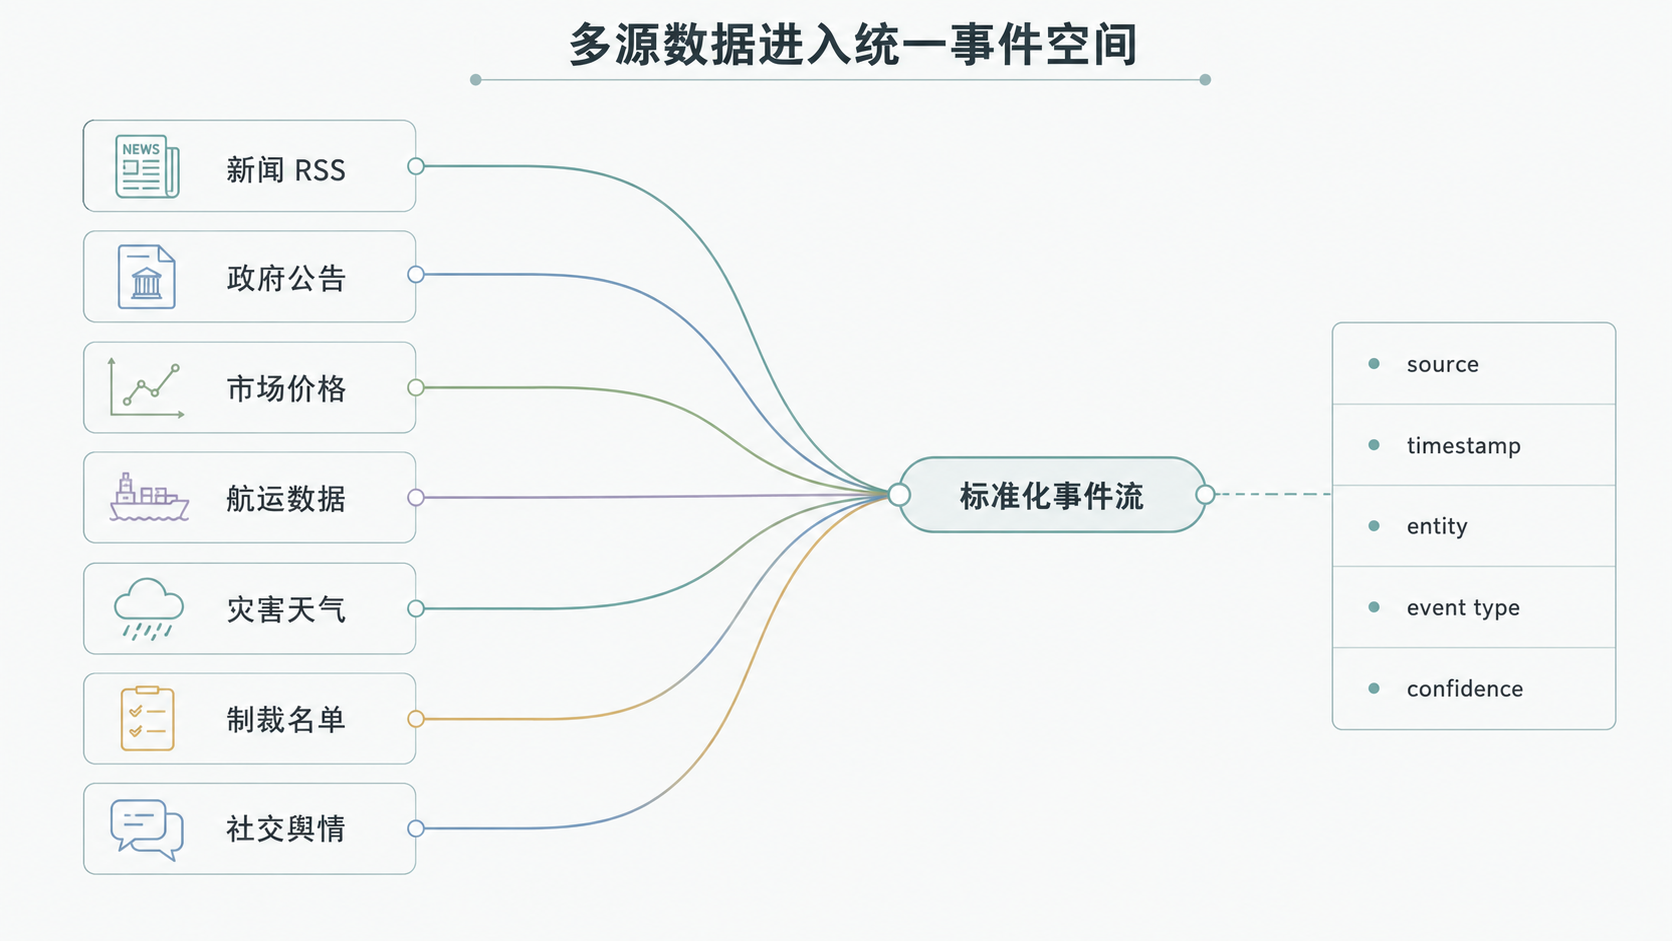
\includegraphics[width=0.95\linewidth]{新增，放在3.2.3 多源数据接入与数据治理.png}
\caption{多源数据接入架构}
\label{fig:data-ingestion}
\end{figure}

系统接入数据可分为七类：全球新闻、政策公告、制裁合规、市场价格、航运物流、气候灾害和社交舆情。不同来源数据在格式、更新频率、可信程度和噪声水平上存在差异，因此需要在进入事件抽取模块之前完成基础治理。

数据治理流程包括：
\begin{enumerate}
    \item \term{采集标准化}：将不同接口返回的数据统一为 \texttt{source}、\texttt{title}、\texttt{content}、\texttt{url}、\texttt{published\_at}、\texttt{language}、\texttt{location} 等字段；
    \item \term{来源注册}：基于 \path{data/lithium/source_registry.json} 维护来源类型、地区、行业相关性和基础信誉度；
    \item \term{内容清洗}：去除 HTML 噪声、重复标题、空正文、无效链接和低质量文本；
    \item \term{时间归一}：将不同格式发布时间统一转换为 ISO 时间格式，并计算事件新鲜度；
    \item \term{实体预召回}：根据锂电池产业链实体别名表识别可能相关的国家、企业、材料、港口和产业环节；
    \item \term{低相关过滤}：过滤与新能源锂电池产业链无关或相关性过低的新闻，降低后续 LLM 调用成本；
    \item \term{缓存与回放}：将关键事件写入本地缓存和样例库，支持演示时离线回放。
\end{enumerate}

数据接入层的目标不是“越多越好”，而是形成面向产业链风险的高质量事件候选池。对于比赛系统而言，可优先保证新闻、政策、制裁、价格和航运五类数据的稳定接入；对于增强版系统，可继续扩展海关贸易、企业财报、专利动态、卫星灾害、社媒情绪等数据源。

\subsubsection{事件抽取与结构化建模}

\begin{figure}[H]
\centering
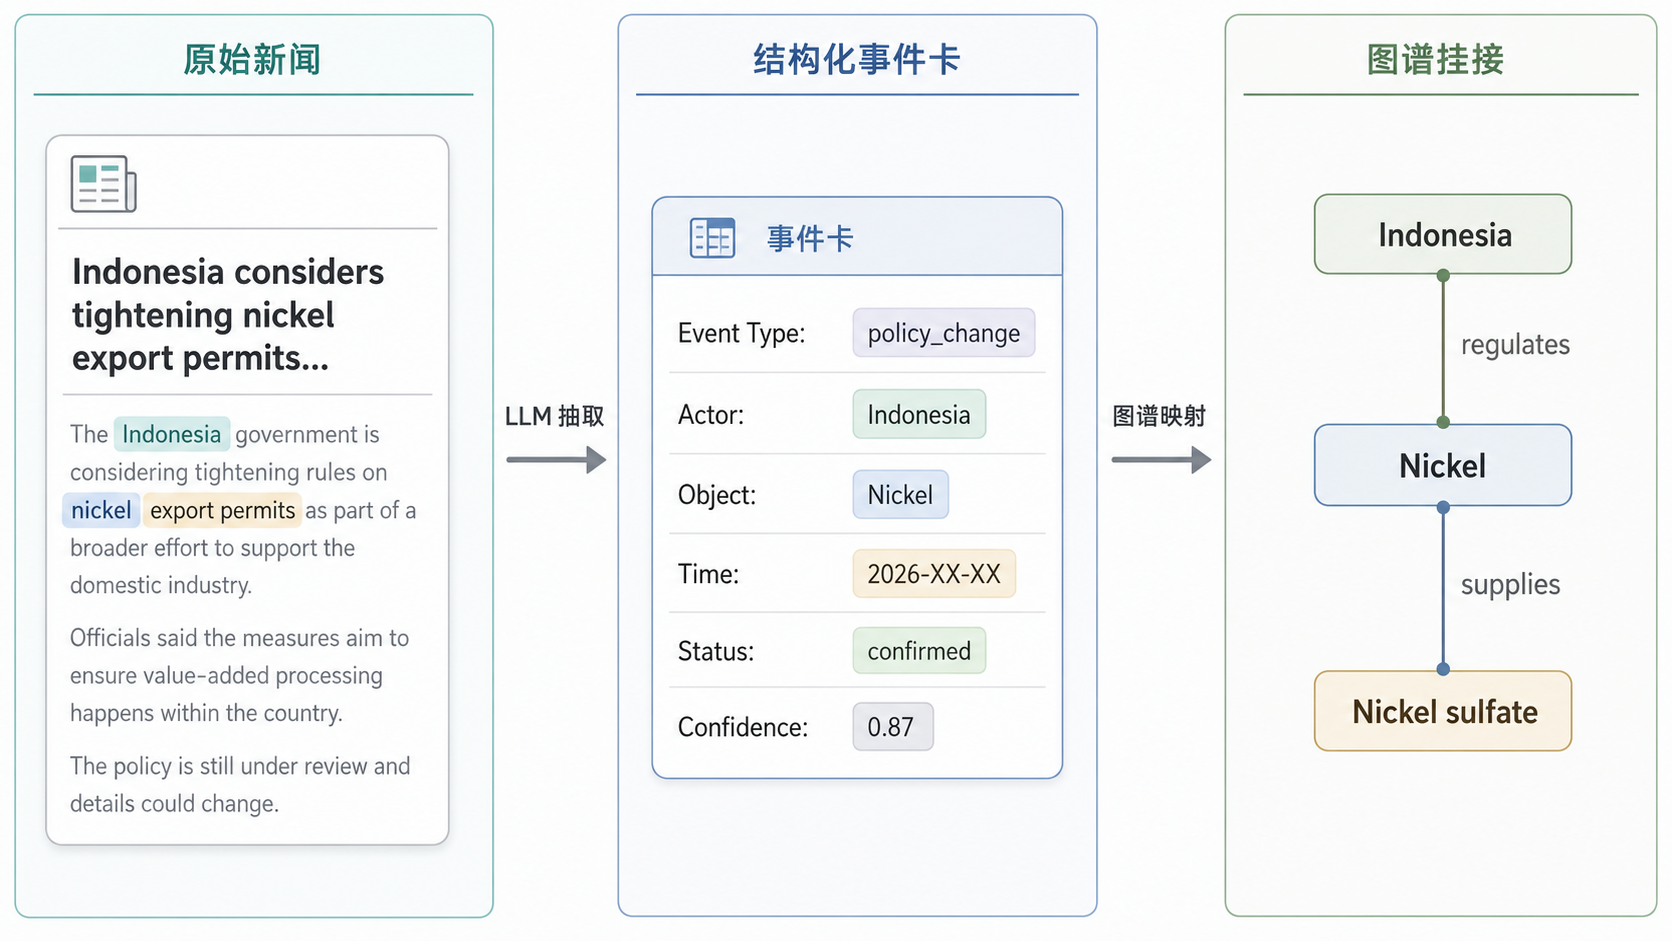
\includegraphics[width=0.95\linewidth]{3.2.4 事件抽取与结构化建模.png}
\caption{事件抽取与结构化建模流程}
\label{fig:event-extraction}
\end{figure}

系统将非结构化文本抽取为标准风险事件对象。事件对象既要满足前端展示需求，也要满足图谱写入和风险评分需求。其核心字段定义如下：
\begin{equation}
e_i =
\left(
t_i, c_i, l_i, \mathcal{E}_i, \mathcal{A}_i, s_i, q_i, u_i, z_i
\right),
\end{equation}
其中，$t_i$ 表示事件发生时间，$c_i$ 表示事件类型，$l_i$ 表示地理位置，$\mathcal{E}_i$ 表示事件涉及实体集合，$\mathcal{A}_i$ 表示受影响产业链节点集合，$s_i$ 表示事件严重度，$q_i$ 表示来源置信度，$u_i$ 表示事件状态，$z_i$ 表示证据集合。

事件类型主要包括：
\begin{itemize}
    \item \texttt{policy\_change}：政策变化；
    \item \texttt{sanction}：制裁与合规风险；
    \item \texttt{supply\_disruption}：供应中断；
    \item \texttt{logistics\_disruption}：物流中断；
    \item \texttt{natural\_disaster}：自然灾害；
    \item \texttt{price\_spike}：价格异常；
    \item \texttt{labor\_strike}：罢工事件；
    \item \texttt{geopolitical\_conflict}：地缘冲突；
    \item \texttt{environment\_regulation}：环保监管；
    \item \texttt{rumor}：传闻与未证实信息。
\end{itemize}

结构化抽取结果示例如下：
\begin{verbatim}
{
  "event_type": "policy_change",
  "event_name": "Indonesia nickel export restriction",
  "time": "2026-06-20",
  "location": "Indonesia",
  "entities": [
    "Indonesia", 
    "Nickel", 
    "Battery Material"
  ],
  "affected_nodes": [
    "nickel", 
    "nickel_sulfate", 
    "cathode_material", 
    "battery_cell"
  ],
  "status": "active",
  "severity": 0.78,
  "confidence": 0.82,
  "summary": "Indonesia announced tighter nickel export controls...",
  "evidence": ["news_001", "policy_003"]
}
\end{verbatim}

为降低抽取错误，系统采用“三重约束”机制。第一，使用事件 Schema 约束输出字段和枚举值，避免 LLM 自由生成不可解析字段。第二，使用产业链实体别名表进行实体对齐，将“印度尼西亚”“印尼”“Indonesia”等不同表述统一映射为同一图谱节点。第三，使用规则校验和置信度阈值过滤异常事件，例如缺少时间、缺少实体、事件类型不合法或严重度超出区间的抽取结果。

\subsubsection{时序可信动态图谱构建}

\begin{figure}[H]
\centering
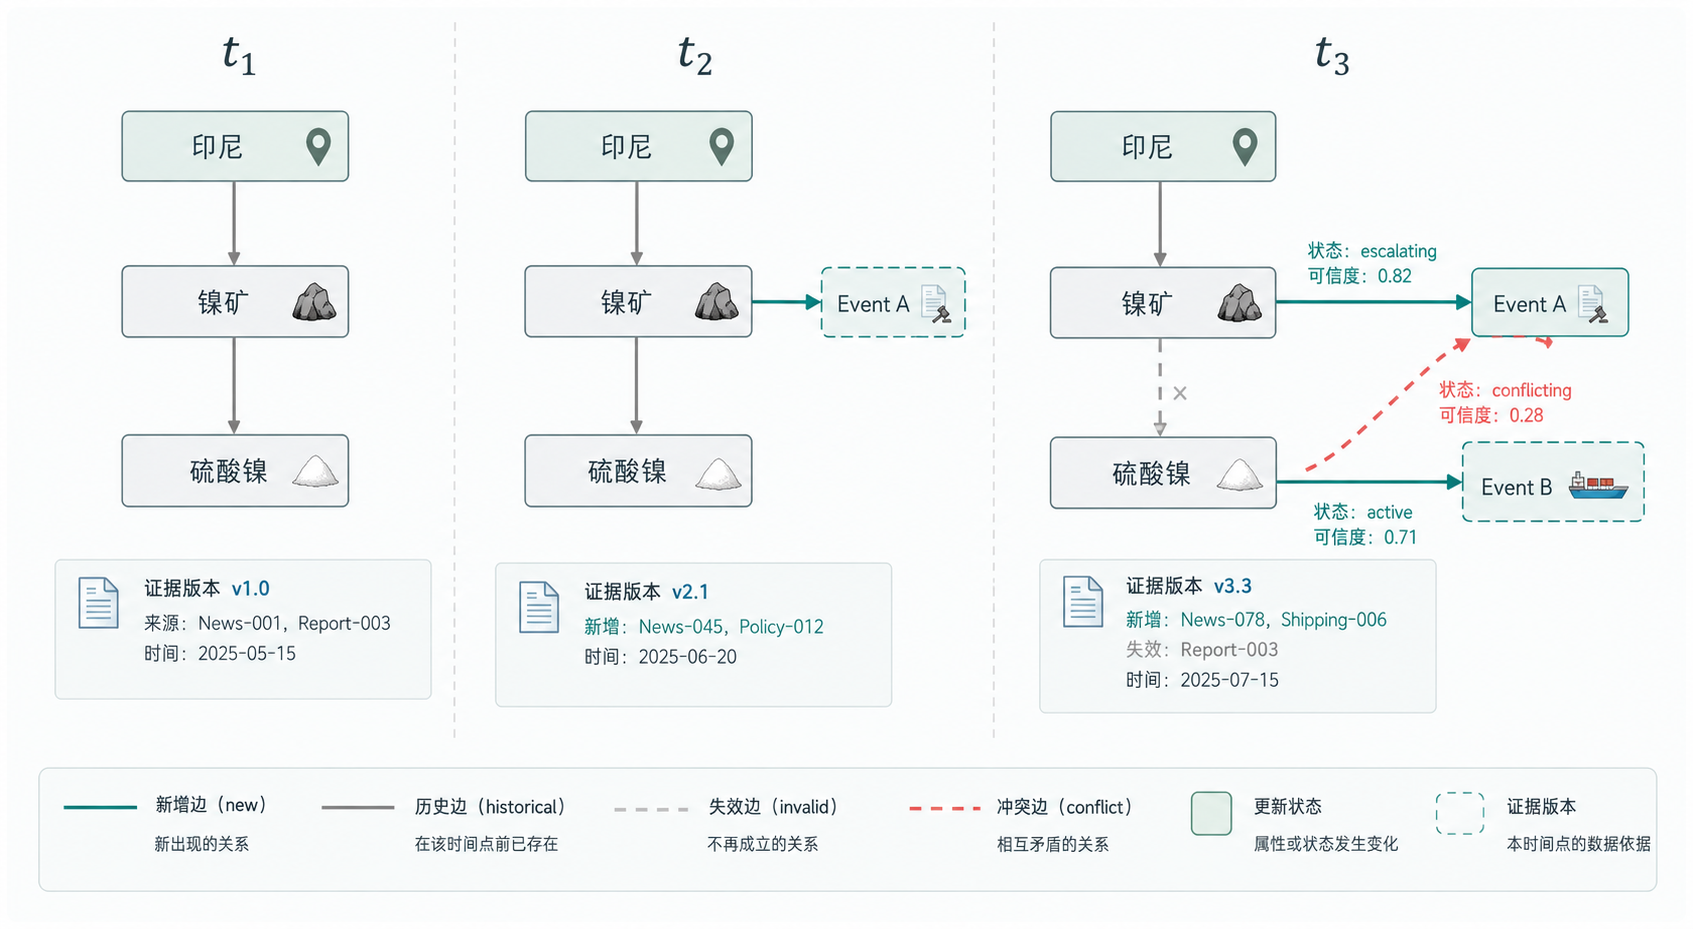
\includegraphics[width=0.95\linewidth]{3.2.5 时序可信动态图谱构建.png}
\caption{时序可信动态图谱构建流程}
\label{fig:temporal-graph}
\end{figure}

普通知识图谱通常将关系表示为静态三元组 $(h,r,t)$，难以表达事件随时间演化、关系失效、冲突修正和风险缓解等动态现象。本项目将产业链图谱扩展为时序可信动态图谱：
\begin{equation}
\mathcal{G}_{\tau} =
\left(
\mathcal{V},
\mathcal{R},
\mathcal{E}_{\tau},
\mathcal{X}_{\tau},
\mathcal{C}_{\tau}
\right),
\end{equation}
其中，$\mathcal{V}$ 为实体节点集合，$\mathcal{R}$ 为关系类型集合，$\mathcal{E}_{\tau}$ 为时间 $\tau$ 下有效的边集合，$\mathcal{X}_{\tau}$ 为事件与证据属性集合，$\mathcal{C}_{\tau}$ 为可信度与状态属性集合。

每条边不再只是“实体—关系—实体”，而是包含如下属性：
\begin{equation}
(h,r,t,\tau_s,\tau_e,\text{status},\text{confidence},\text{evidence}),
\end{equation}
其中，$\tau_s$ 和 $\tau_e$ 分别表示关系生效时间和失效时间；\texttt{status} 表示当前状态；\texttt{confidence} 表示可信度；\texttt{evidence} 表示支撑该关系的证据来源。

事件状态机定义如下：
\begin{figure}[H]
\centering
\resizebox{\linewidth}{!}{
\begin{tikzpicture}[
    font=\scriptsize,
    state/.style={rectangle, rounded corners=3pt, draw=DeepBlue, thick, fill=SoftBlue, minimum width=1.75cm, minimum height=0.65cm, align=center},
    bad/.style={rectangle, rounded corners=3pt, draw=LineGray, thick, fill=SoftRed, minimum width=1.75cm, minimum height=0.65cm, align=center},
    good/.style={rectangle, rounded corners=3pt, draw=LineGray, thick, fill=Mint, minimum width=1.75cm, minimum height=0.65cm, align=center},
    arrow/.style={-{Latex[length=2mm]}, thick, draw=LineGray}
]
\node[state] (rumor) {rumor\\传闻};
\node[state, right=0.55cm of rumor] (confirmed) {confirmed\\已确认};
\node[state, right=0.55cm of confirmed] (escalating) {escalating\\升级中};
\node[state, right=0.55cm of escalating] (active) {active\\影响中};
\node[good, right=0.55cm of active] (mitigating) {mitigating\\缓解中};
\node[good, right=0.55cm of mitigating] (resolved) {resolved\\已解决};
\node[bad, below=0.75cm of confirmed] (invalid) {invalidated\\被证伪};
\node[bad, below=0.75cm of active] (conflict) {conflicting\\冲突};

\draw[arrow] (rumor) -- (confirmed);
\draw[arrow] (confirmed) -- (escalating);
\draw[arrow] (escalating) -- (active);
\draw[arrow] (active) -- (mitigating);
\draw[arrow] (mitigating) -- (resolved);
\draw[arrow] (rumor) |- (invalid);
\draw[arrow] (confirmed) -- (invalid);
\draw[arrow] (active) -- (conflict);
\draw[arrow] (conflict) -| (mitigating);
\end{tikzpicture}
}
\caption{风险事件时序状态机}
\label{fig:event-state-machine}
\end{figure}

该状态机使系统能够回答传统 RAG 难以稳定回答的问题，例如：“该事件当前是否仍然有效？”“风险是升级、缓解还是终止？”“过去三个月风险如何演化？”“某条产业链关系是否已经被后续信息修正？”通过将状态变化写入历史记录，系统可以生成事件演化链，并支持按时间点回放产业链风险态势。

\subsubsection{Trust Graph 可信度评估与冲突消解}

开放互联网数据存在来源复杂、重复报道、断章取义、滞后更新和信息冲突等问题。为避免系统被单一低可信来源误导，本项目设计 Trust Graph 可信度机制，将来源信誉、跨源一致性、实体匹配度和时间接近度共同纳入事件置信度计算。

事件置信度定义为：
\begin{equation}
Q(e_i)=
\alpha R_{\text{src}}(e_i)
+
\beta R_{\text{cons}}(e_i)
+
\gamma R_{\text{ent}}(e_i)
+
\delta R_{\text{time}}(e_i),
\end{equation}
其中，$R_{\text{src}}$ 表示来源基础信誉度，$R_{\text{cons}}$ 表示多源一致性，$R_{\text{ent}}$ 表示实体匹配准确度，$R_{\text{time}}$ 表示时间接近度。默认权重可设置为：
\begin{equation}
\alpha=0.4,\quad \beta=0.3,\quad \gamma=0.2,\quad \delta=0.1.
\end{equation}

来源基础信誉度可按如下原则初始化：
\begin{center}
\begin{tabularx}{0.95\linewidth}{>{\raggedright\arraybackslash}X c >{\raggedright\arraybackslash}X}
\toprule
来源类型 & 基础信誉度 & 说明 \\
\midrule
政府机构/官方公告 & 0.92--0.98 & 适合用于政策、制裁、监管和官方声明确认 \\
主流媒体 & 0.80--0.90 & 适合用于重大新闻和公开事件确认 \\
行业媒体 & 0.70--0.82 & 适合用于产业链细节、企业动态和价格扰动解释 \\
金融媒体 & 0.68--0.80 & 适合用于市场预期、价格影响和资本市场反应 \\
社交媒体 & 0.35--0.55 & 适合用于早期信号发现，但需要交叉验证 \\
匿名爆料 & 0.15--0.35 & 仅作为弱信号，不直接触发高置信预警 \\
\bottomrule
\end{tabularx}
\end{center}

当多源信息冲突时，系统触发多 Agent 冲突消解机制。不同 Agent 分别从官方证据、主流媒体、行业逻辑、市场数据和社交舆情角度对事件进行校验，并输出支持、反驳或不确定判断。

以下是一个具体的冲突消解示例。假设系统同时接收到两条关于"印尼镍出口政策"的信息：

来源 A（政府官网，信誉度 0.95）称："印尼能矿部正在研究镍出口限制方案，尚未做出决定。"
来源 B（行业媒体，信誉度 0.78）称："印尼已确定将于下月起实施镍出口禁令。"

四个 Agent 分别做出判断：
\begin{itemize}
    \item 官方证据 Agent：采信来源 A，指出来源 B 的说法与官方公告矛盾。
    \item 媒体一致性 Agent：检查后发现除来源 B 外，其他主流媒体均未报道"已确定实施"——来源 B 可能为独家消息或误报。
    \item 行业逻辑 Agent：指出印尼过去对镍出口的政策调整通常有 3--6 个月的过渡期，"下月立即实施"不符合惯例。
    \item 噪声识别 Agent：来源 B 的报道语言偏 sensational（使用了"重磅""突然宣布"等词），且未直接引用官方文件编号，可信度存疑。
\end{itemize}

冲突裁决器综合四个 Agent 的输出，将事件标记为 conflicting 状态，置信度下调至 0.55，并在证据字段中注明"政府官网称正在研究，行业媒体称已确定实施，存在矛盾"。该事件不会参与紧急风险评分，但会保留在监控列表中——如果后续有更多来源（如印尼官方正式文件）确认，可以升级为 confirmed。

冲突消解结果不简单删除争议信息，而是将其标记为 \texttt{confirmed}、\texttt{conflicting}、\texttt{unverified}、\texttt{resolved} 或 \texttt{invalidated}，供后续风险评分和报告生成使用。

\begin{figure}[H]
\centering
\resizebox{\linewidth}{!}{
\begin{tikzpicture}[
    font=\scriptsize,
    node distance=0.65cm,
    src/.style={rectangle, rounded corners=3pt, draw=DeepBlue, fill=SoftBlue, thick, align=center, minimum width=2.2cm, minimum height=0.65cm},
    agent/.style={rectangle, rounded corners=3pt, draw=TechBlue, fill=Mint, thick, align=center, minimum width=2.2cm, minimum height=0.65cm},
    outnode/.style={rectangle, rounded corners=3pt, draw=LineGray, fill=SoftOrange, thick, align=center, minimum width=2.5cm, minimum height=0.65cm},
    arrow/.style={-{Latex[length=2mm]}, thick, draw=LineGray}
]
\node[src] (official) {官方公告\\高可信};
\node[src, below=of official] (media) {主流媒体\\跨源报道};
\node[src, below=of media] (industry) {行业媒体\\产业细节};
\node[src, below=of industry] (social) {社交舆情\\早期信号};

\node[agent, right=1.0cm of official] (a1) {官方证据 Agent};
\node[agent, right=1.0cm of media] (a2) {媒体一致性 Agent};
\node[agent, right=1.0cm of industry] (a3) {行业逻辑 Agent};
\node[agent, right=1.0cm of social] (a4) {噪声识别 Agent};

\node[outnode, right=1.1cm of a2, yshift=-0.35cm] (judge) {冲突裁决器\\Confidence Score};
\node[outnode, right=1.0cm of judge] (result) {可信事件链\\状态+置信度+证据};

\draw[arrow] (official) -- (a1);
\draw[arrow] (media) -- (a2);
\draw[arrow] (industry) -- (a3);
\draw[arrow] (social) -- (a4);
\draw[arrow] (a1) -- (judge);
\draw[arrow] (a2) -- (judge);
\draw[arrow] (a3) -- (judge);
\draw[arrow] (a4) -- (judge);
\draw[arrow] (judge) -- (result);
\end{tikzpicture}
}
\caption{Trust Graph 驱动的多 Agent 冲突消解机制}
\label{fig:trust-agent}
\end{figure}

\subsubsection{图拓扑增强的风险传播推理}

新能源锂电池产业链风险通常不是孤立事件，而是沿着“资源—材料—制造—应用—市场”的链条传播。例如，印尼镍矿出口限制可能首先影响镍矿供应，再传导至镍中间品、硫酸镍、三元正极材料、电芯成本和新能源汽车企业利润。为建模这种链式传播，本项目在图谱上执行风险传播搜索。

设事件 $e_i$ 命中的初始节点集合为 $\mathcal{S}_i$，产业链图谱为 $\mathcal{G}_{\tau}$。系统从 $\mathcal{S}_i$ 出发搜索长度不超过 $K$ 的传播路径：
\begin{equation}
p=(v_0,r_1,v_1,\cdots,r_k,v_k), \quad k \le K,
\end{equation}
其中 $v_0 \in \mathcal{S}_i$，$r_j$ 表示产业链依赖关系、供应关系、替代关系、物流关系或政策影响关系。路径传播强度定义为：
\begin{equation}
I(p)=s_i \cdot Q(e_i) \cdot
\prod_{j=1}^{k} w(r_j) \cdot
\exp(-\lambda k),
\end{equation}
其中，$s_i$ 为事件严重度，$Q(e_i)$ 为事件置信度，$w(r_j)$ 为关系权重，$\exp(-\lambda k)$ 为路径长度衰减项。

节点关键性由多个拓扑指标融合得到：
\begin{equation}
K(v)=
\eta_1 \text{PR}(v)
+
\eta_2 \text{Deg}(v)
+
\eta_3 \text{Bet}(v)
+
\eta_4 \text{Com}(v),
\end{equation}
其中，$\text{PR}(v)$ 表示 PageRank，$\text{Deg}(v)$ 表示度中心性，$\text{Bet}(v)$ 表示介数中心性，$\text{Com}(v)$ 表示社区桥接或产业链跨层连接能力。对于锂、镍、钴、石墨、马六甲海峡、红海、宁德时代、比亚迪、特斯拉等关键节点，系统可以根据拓扑关键性自动提升风险关注等级。

\begin{figure}[H]
\centering
\resizebox{\linewidth}{!}{
\begin{tikzpicture}[
    font=\scriptsize,
    node distance=0.72cm,
    v/.style={circle, draw=DeepBlue, thick, fill=SoftBlue, minimum size=0.9cm, align=center},
    risk/.style={circle, draw=TechBlue, thick, fill=SoftRed, minimum size=0.95cm, align=center},
    mid/.style={circle, draw=LineGray, thick, fill=Mint, minimum size=0.9cm, align=center},
    arrow/.style={-{Latex[length=2mm]}, thick, draw=LineGray}
]
\node[risk] (event) {事件\\政策};
\node[v, right=0.9cm of event] (nickel) {镍矿};
\node[v, right=0.9cm of nickel] (sulfate) {硫酸镍};
\node[mid, right=0.9cm of sulfate] (cathode) {三元\\正极};
\node[mid, right=0.9cm of cathode] (cell) {电芯};
\node[mid, right=0.9cm of cell] (ev) {整车};
\node[v, below=0.75cm of sulfate] (price) {价格};
\node[v, below=0.75cm of cathode] (company) {企业\\利润};

\draw[arrow] (event) -- node[above] {命中} (nickel);
\draw[arrow] (nickel) -- node[above] {供应} (sulfate);
\draw[arrow] (sulfate) -- node[above] {材料} (cathode);
\draw[arrow] (cathode) -- node[above] {制造} (cell);
\draw[arrow] (cell) -- node[above] {应用} (ev);
\draw[arrow] (sulfate) -- (price);
\draw[arrow] (price) -- (company);
\draw[arrow] (cathode) -- (company);
\end{tikzpicture}
}
\caption{锂电池产业链风险传播路径示意}
\label{fig:risk-propagation}
\end{figure}

该机制使系统不只是回答“发生了什么”，而是进一步回答“影响谁、沿什么路径影响、影响强度多大、哪些节点最值得关注”。这也是本项目相较于普通新闻问答系统和传统 RAG 系统的核心竞争力之一。
从实现角度来看，搜索算法同时支持 BFS 和 DFS 两种模式。BFS 模式用于快速评估风险的影响广度——从源节点出发逐层扩展，优先发现所有可能受影响的节点和环节，适合"这个事件影响范围有多大"这类问题。DFS 模式用于深入评估特定路径的影响深度——沿着一条路径一直搜索到最下游，适合"这个事件最终会影响到哪个终端市场"这类问题。两种模式共用同一个带权有向图结构，差异仅在于节点遍历顺序和剪枝条件。

搜索过程还包含三个实际的工程优化。第一，路径去重：同一条物理路径可能通过不同顺序的节点遍历被发现多次，系统在路径生成阶段使用哈希集合去重。第二，环路检测：产业链图谱中可能存在循环依赖（如A$\to$B$\to$C$\to$A），搜索过程中维护已访问节点集合，遇到重复节点时终止当前路径。第三，早期终止：当路径强度衰减到预设阈值以下时（$I(p) < 0.05$），即使未达到最大深度也提前终止搜索，避免无效计算。



\subsubsection{可解释风险评分模型}

为避免大语言模型直接给出主观判断，本项目设计可解释风险评分模型。综合风险分数定义为：
\begin{equation}
\text{RiskScore}(e_i)=100 \cdot
\left[
\omega_1 S(e_i)
+
\omega_2 K(\mathcal{A}_i)
+
\omega_3 Q(e_i)
+
\omega_4 P(e_i)
+
\omega_5 T(e_i)
\right],
\end{equation}
其中，$S(e_i)$ 表示事件严重度，$K(\mathcal{A}_i)$ 表示受影响节点关键性，$Q(e_i)$ 表示来源置信度，$P(e_i)$ 表示传播影响范围，$T(e_i)$ 表示时间新鲜度。默认权重为：
\begin{equation}
\omega_1=0.35,\quad
\omega_2=0.25,\quad
\omega_3=0.20,\quad
\omega_4=0.15,\quad
\omega_5=0.05.
\end{equation}

其中，时间新鲜度可定义为：
\begin{equation}
T(e_i)=\exp\left(-\frac{\Delta t_i}{\theta}\right),
\end{equation}
$\Delta t_i$ 表示当前时间与事件发生时间之间的间隔，$\theta$ 为时间衰减系数。传播影响范围可由受影响节点数、路径强度和跨产业层级数量共同确定：
\begin{equation}
P(e_i)=
\min\left(
1,
\frac{|\mathcal{V}_{\text{affected}}|}{M}
\right)
\cdot
\frac{1}{|\mathcal{P}_i|}
\sum_{p \in \mathcal{P}_i} I(p),
\end{equation}
其中，$\mathcal{V}_{\text{affected}}$ 表示受影响节点集合，$M$ 为归一化常数，$\mathcal{P}_i$ 为传播路径集合。

风险等级划分如下：
\begin{center}
\begin{tabularx}{0.9\linewidth}{c c >{\raggedright\arraybackslash}X}
\toprule
风险分数 & 风险等级 & 处置建议 \\
\midrule
0--30 & 低风险 & 纳入常规监测，保留事件记录和证据来源 \\
31--60 & 中风险 & 提升监测频率，关注后续政策、价格和企业响应 \\
61--80 & 高风险 & 生成重点预警，跟踪传播路径和关键节点变化 \\
81--100 & 紧急风险 & 触发高级告警，生成专项研判报告和应急建议 \\
\bottomrule
\end{tabularx}
\end{center}

最终输出结果包括风险分数、风险等级、置信度、影响路径、关键证据、历史演化和应对建议。该评分机制将复杂产业链风险转化为可解释量化结果，便于企业、金融机构和监管部门进行快速决策。

\subsubsection{图增强大语言模型研判}

本项目中的 LLM 研判模块采用 Graph-enhanced Prompt 方式，不让大模型直接从原文中自由推理，而是将图谱计算得到的结构化证据包输入模型。输入内容包括：
\begin{itemize}
    \item 风险事件摘要和事件类型；
    \item 事件发生时间、状态和时间新鲜度；
    \item 命中产业链节点和实体对齐结果；
    \item Trust Graph 置信度和冲突状态；
    \item 风险传播路径和关键节点；
    \item 综合风险评分及各分项贡献；
    \item 支撑证据来源和证据摘要；
    \item 历史相似案例和后续监控重点。
\end{itemize}

报告生成目标不是生成泛泛而谈的新闻摘要，而是生成面向产业链决策的“风险穿透研判报告”。报告结构如下：
\begin{enumerate}
    \item 事件概述：说明事件发生背景、核心事实和当前状态；
    \item 风险类型：判断事件属于政策、供应、物流、价格、制裁还是灾害风险；
    \item 影响路径：展示风险从初始节点向上下游传导的路径；
    \item 关键节点：指出受影响程度最高的国家、材料、企业或物流通道；
    \item 风险评分：给出综合分数、风险等级和置信度；
    \item 证据链：列出支撑结论的主要信息来源和一致性判断；
    \item 潜在影响：分析未来 1--3 个月可能影响；
    \item 应对建议：从采购、库存、替代供应、合规审查和持续监控角度提出建议。
\end{enumerate}

示例研判风格如下：
\begin{quote}
印尼镍矿出口限制事件当前处于 \texttt{active} 状态，综合风险评分为 82，风险等级为高。该事件直接影响镍矿供应，并沿产业链传导至硫酸镍、三元正极材料和动力电池环节。由于镍节点在产业链中的关键性较高，且多个高可信来源已确认政策收紧，系统判断该事件可能在未来 1--3 个月内对三元电池材料成本形成上行压力。建议重点关注印尼政策执行细则、国内硫酸镍价格变化以及高镍三元电池企业采购策略。
\end{quote}

\subsubsection{可视化展示与交互设计}

系统前端围绕“风险发现、风险解释、风险追踪、风险汇报”四类任务设计。核心页面包括：
\begin{itemize}
    \item \term{全球风险地图}：展示事件发生地、影响地区和传播范围；
    \item \term{产业链图谱视图}：展示国家、材料、企业、物流通道和产业环节之间的关系；
    \item \term{风险事件时间线}：展示事件从 rumor 到 confirmed、active、mitigating、resolved 的演化过程；
    \item \term{风险节点排行榜}：按照风险分数、节点关键性和影响频次排序；
    \item \term{风险传播路径图}：展示事件如何沿产业链上下游传导；
    \item \term{证据来源面板}：展示不同来源的可信度、时间和一致性；
    \item \term{AI 研判报告面板}：自动生成可复制、可下载、可汇报的风险分析文本。
\end{itemize}

前端演示重点突出“可看、可点、可追溯”。用户输入一个事件或选择一个风险案例后，系统应能在数秒内完成事件结构化、图谱命中、传播路径搜索、风险评分和报告生成，并在页面上同步展示图谱和文字解释。相比单纯问答系统，该交互方式更符合产业风险监测场景，也更容易在比赛答辩中展示技术深度和工程完成度。

\subsubsection{实验评估与技术指标}

为证明系统效果，本项目拟设计普通 RAG、静态知识图谱 RAG 和本项目 Temporal Trust Graph RAG 三类对比方案。评估指标包括：
\begin{center}
\begin{tabularx}{0.95\linewidth}{>{\raggedright\arraybackslash}p{3.2cm} >{\raggedright\arraybackslash}p{3.6cm} >{\raggedright\arraybackslash}X}
\toprule
指标类别 & 指标名称 & 说明 \\
\midrule
事件抽取能力 & 字段完整率、实体匹配率、事件类型准确率 & 衡量系统将非结构化文本转为结构化事件的能力 \\
时间感知能力 & 过期关系识别率、状态演化准确率 & 衡量系统判断事件是否仍然有效的能力 \\
可信判断能力 & 冲突识别率、置信度校准误差 & 衡量系统对多源噪声和冲突信息的处理能力 \\
传播推理能力 & 路径命中率、关键节点召回率 & 衡量系统识别产业链影响路径的能力 \\
报告质量 & 可解释性、证据一致性、人工评分 & 衡量 AI 研判报告是否可信、完整、可读 \\
系统性能 & 响应时间、缓存命中率、演示稳定性 & 衡量系统在比赛现场的可运行性 \\
\bottomrule
\end{tabularx}
\end{center}

项目预期目标是：在典型样例集上，Temporal Trust Graph RAG 相比普通 RAG 能够显著提升过期信息识别能力、风险传播路径完整性和报告可解释性；在开放新闻环境中，Trust Graph 能够降低单一低可信来源造成的误报；在展示层面，系统能够形成从事件输入到风险报告输出的完整闭环。

\subsection{计划和分工}

\subsubsection{总体实施计划}

本项目计划按照“场景定义—数据体系—图谱建模—可信推理—智能研判—可视化展示—实验评估”的路线推进。整体实施强调从零搭建、自主设计和逐步迭代，确保系统不仅能够完成比赛演示，还能够充分体现技术原创性、工程完整性和产业应用价值。

需要说明的是，项目当前已完成核心原型代码建设，因此后续实施计划不再是从零启动，而是围绕“功能加固、数据扩展、交互优化、实验评估和比赛展示”展开。当前代码已经覆盖事件 Schema、图谱推理、Trust Graph、风险评分、市场监测、报告生成和 Dashboard 适配等关键模块，后续重点是提高数据覆盖率、增强演示稳定性、补充对比实验和打磨答辩叙事。

\begin{center}
\begin{longtable}{p{2.2cm} p{3.2cm} p{7.2cm}}
\toprule
阶段 & 阶段目标 & 主要任务 \\
\midrule
第一阶段 & 需求分析与场景定义 & 明确新能源锂电池产业链风险预警任务；确定系统功能边界；定义风险事件类型、产业链节点类型、图谱关系类型和预警输出形式。 \\
第二阶段 & 产业链知识库自主构建 & 从公开资料和行业知识中整理国家、材料、企业、产业环节、物流通道和风险类型；构建实体别名表、关系类型表和初始产业链图谱。 \\
第三阶段 & 多源数据采集体系搭建 & 自主开发新闻、公告、制裁、价格、航运、灾害和舆情数据接入模块；统一数据格式；完成数据清洗、去重、时间归一和来源注册。 \\
第四阶段 & 风险事件抽取与结构化 & 设计事件抽取 Prompt 和字段约束 Schema；实现实体识别、实体对齐、事件类型分类、严重度判断、证据绑定和异常字段校验。 \\
第五阶段 & 时序动态图谱构建 & 为图谱节点、边和事件增加时间戳、有效期、状态和历史版本；实现事件状态机、历史回溯查询和事件演化链追踪。 \\
第六阶段 & Trust Graph 与冲突消解 & 建立来源信誉评分表；实现多源一致性判断、实体匹配置信度、时间接近度计算和冲突事件标记；输出可解释置信度。 \\
第七阶段 & 风险传播推理与评分 & 实现产业链影响路径搜索；计算节点关键性、传播范围、时间新鲜度和综合风险分数；输出风险等级、关键节点和传播路径。 \\
第八阶段 & LLM 研判报告生成 & 将事件摘要、图谱路径、风险评分、可信度和证据链组织为结构化 Prompt；生成可解释、可追溯、可汇报的产业链风险研判报告。 \\
第九阶段 & Web 可视化系统开发 & 自主开发风险地图、产业链图谱、时间线、节点榜单、证据面板和报告面板；完成端到端交互演示。 \\
第十阶段 & 实验评估与答辩准备 & 设计普通 RAG、静态图谱 RAG 和本项目方案的对比实验；整理案例、截图、演示视频、技术报告和答辩 PPT。 \\
\bottomrule
\end{longtable}
\end{center}

\subsubsection{阶段里程碑}

项目里程碑设计如下：
\begin{figure}[H]
\centering
\resizebox{\linewidth}{!}{
\begin{tikzpicture}[
    font=\scriptsize,
    mile/.style={rectangle, rounded corners=3pt, draw=DeepBlue, thick, fill=SoftBlue, align=center, minimum width=2.05cm, minimum height=0.75cm},
    done/.style={rectangle, rounded corners=3pt, draw=TechBlue, thick, fill=Mint, align=center, minimum width=2.05cm, minimum height=0.75cm},
    arrow/.style={-{Latex[length=2mm]}, thick, draw=LineGray}
]
\node[done] (m1) {M1\\图谱种子库};
\node[mile, right=0.35cm of m1] (m2) {M2\\事件抽取};
\node[mile, right=0.35cm of m2] (m3) {M3\\时序状态机};
\node[mile, right=0.35cm of m3] (m4) {M4\\Trust Graph};
\node[mile, right=0.35cm of m4] (m5) {M5\\风险评分};
\node[mile, right=0.35cm of m5] (m6) {M6\\可视化 Demo};
\node[mile, right=0.35cm of m6] (m7) {M7\\答辩材料};

\draw[arrow] (m1) -- (m2);
\draw[arrow] (m2) -- (m3);
\draw[arrow] (m3) -- (m4);
\draw[arrow] (m4) -- (m5);
\draw[arrow] (m5) -- (m6);
\draw[arrow] (m6) -- (m7);
\end{tikzpicture}
}
\caption{项目阶段里程碑}
\label{fig:milestone}
\end{figure}

其中，M1 和 M2 决定系统能否形成有效数据闭环；M3 和 M4 决定项目是否具备区别于普通 RAG 的技术亮点；M5 决定风险结果是否可解释；M6 和 M7 决定比赛展示效果。项目推进过程中应优先保证 M1--M5 的稳定性，再逐步增强可视化效果和答辩包装。

\subsubsection{团队分工}

结合项目技术模块，团队可划分为六类角色。每一类角色均围绕自研系统建设展开，分别负责数据、图谱、算法、模型、后端和前端等关键部分。团队人数较少时，由一名成员承担多个角色，但需要保证每个核心模块均有明确负责人。

\begin{center}
\begin{tabularx}{0.95\linewidth}{p{2.6cm} p{3.4cm} X}
\toprule
角色 & 负责模块 & 主要职责 \\
\midrule
项目负责人 & 总体架构与答辩统筹 & 确定项目定位、技术路线、系统边界和比赛叙事；协调各模块进度；统一文档、PPT、演示脚本和答辩口径。 \\
数据工程成员 & 多源数据采集与治理 & 自主开发新闻、公告、制裁、价格、航运、灾害和舆情数据接入模块；完成数据清洗、去重、时间归一、来源注册和样例数据维护。 \\
知识工程成员 & 产业链知识图谱构建 & 整理新能源锂电池产业链实体、关系、别名、风险类型和样例事件；维护 \path{data/kg_seed/}、\path{data/entity_alias/} 和 \path{config/risk_event_schema.json}。 \\
算法成员 & Trust Graph 与风险推理 & 实现来源可信度计算、多源一致性判断、冲突消解、图传播路径搜索、节点关键性计算和综合风险评分模型。 \\
大模型成员 & 事件抽取与报告生成 & 设计事件抽取 Prompt、结构化输出约束、证据归纳 Prompt、研判报告模板和大模型调用缓存策略。 \\
后端工程成员 & API 与服务编排 & 搭建后端服务，封装数据接口、事件接口、图谱接口、评分接口和报告接口；实现日志、缓存、配置管理和异常处理。 \\
前端展示成员 & Dashboard 与交互可视化 & 自主开发全球风险地图、产业链图谱、风险时间线、风险节点榜、证据链面板和 AI 研判报告面板。 \\
测试与材料成员 & 实验评估与比赛交付 & 构建对比实验、人工评测表和典型案例；整理项目报告、答辩 PPT、演示视频、系统截图和问答材料。 \\
\bottomrule
\end{tabularx}
\end{center}

分工原则是“场景牵引、图谱为核、可信增强、模型辅助、展示闭环”。数据工程和知识工程提供系统底座；算法成员负责项目技术亮点；大模型成员负责将结构化证据转化为可读研判；后端和前端成员负责将算法能力产品化；测试与材料成员保证比赛展示和答辩表达效果。

\subsubsection{进度安排}

项目计划可按“已实现原型巩固 + 比赛级展示增强”的思路推进。由于系统的核心后端模块和前端数据适配已基本形成，后续工作重点不再是基础功能开发，而是围绕数据源扩展、规则校准、图谱补全、前端交互优化、实验验证和答辩材料进行集中打磨。

\begin{center}
\begin{tabularx}{0.95\linewidth}{c X X}
\toprule
周次 & 重点任务 & 交付物 \\
\midrule
第 1 周 & 明确需求边界，设计系统总体架构，定义产业链节点、关系和风险事件类型 & 需求说明、总体架构图、事件类型表、图谱 Schema 初版 \\
第 2 周 & 自主构建产业链知识库，整理关键国家、材料、企业、物流通道和产业环节 & \path{data/kg_seed/}、实体别名表、关系类型表、风险类型配置 \\
第 3 周 & 开发多源数据采集模块，完成新闻、政策、制裁、价格和航运数据的统一接入 & 数据采集接口、标准文档对象、来源注册表、样例原文库 \\
第 4 周 & 开发事件抽取模块，实现字段约束、实体对齐、事件去重和异常校验 & 事件抽取 Prompt、事件 Schema 校验器、结构化事件样例库 \\
第 5 周 & 开发时序动态图谱模块和事件状态机，实现关系有效期、状态更新和历史追踪 & 时序图谱模块、事件状态机、历史事件链查询接口 \\
第 6 周 & 开发 Trust Graph、冲突消解和风险传播评分模块 & 可信度计算模块、冲突识别模块、传播路径搜索模块、风险评分 API \\
第 7 周 & 开发 LLM 研判报告模块和 Web 可视化系统，完成前后端联调 & Dashboard Demo、风险地图、图谱视图、时间线、报告生成面板 \\
第 8 周 & 完成对比实验、系统优化、演示脚本、项目报告、PPT 和答辩材料 & 完整演示系统、实验结果、演示视频、技术报告、答辩 PPT \\
\bottomrule
\end{tabularx}
\end{center}

\subsubsection{质量保障与风险预案}

由于本项目从零搭建完整系统，实施过程中可能面临数据源波动、事件抽取错误、图谱不完整、可信度规则偏差、前端展示复杂和现场网络不稳定等风险。为保证项目最终能够稳定演示并体现技术完整性，系统设计以下质量保障机制。

\begin{itemize}
    \item \term{数据源风险}：建立实时采集与离线样例双模式。实时采集用于展示系统开放环境适应能力，离线样例用于保证比赛现场在网络异常或第三方接口不可用时仍能完整演示。
    \item \term{抽取错误风险}：采用固定事件 Schema、字段合法性校验、实体别名表、枚举类型约束和人工抽样复核，降低大语言模型抽取不稳定带来的错误。
    \item \term{图谱稀疏风险}：初期优先覆盖锂、镍、钴、石墨、正极、负极、电芯、整车、储能、红海、马六甲海峡等高风险高频节点，确保核心案例能够形成完整传播路径。
    \item \term{可信度偏差风险}：来源信誉度采用可配置规则，不将单一来源作为最终判断依据，而是综合来源类型、多源一致性、实体匹配度和时间接近度进行置信度计算。
    \item \term{模型幻觉风险}：限制大语言模型直接生成未经证据支持的判断。所有报告结论必须绑定事件状态、风险分数、传播路径和证据来源。
    \item \term{系统集成风险}：采用模块化接口和标准 JSON 对象传递，确保数据接入、事件抽取、图谱推理、风险评分和前端展示可以分别测试、逐步联调。
    \item \term{前端展示风险}：优先保证事件列表、风险评分、传播路径和报告面板稳定，再逐步增强地图动画、图谱交互和高级视觉效果。
    \item \term{答辩展示风险}：准备标准演示脚本、典型案例截图、离线演示视频和常见问答材料，保证现场展示具有可控性和稳定性。
\end{itemize}

通过上述质量保障机制，本项目能够在自主搭建完整系统的同时降低工程不确定性，确保核心技术模块可运行、可解释、可展示。

\subsubsection{预期成果}

项目完成后预计形成以下成果：
\begin{enumerate}
    \item 一套面向新能源锂电池产业链的黑天鹅风险推理与预警系统；
    \item 一个覆盖国家、材料、企业、产业环节、物流通道和风险类型的产业链知识图谱；
    \item 一个多源风险事件采集与结构化抽取模块；
    \item 一个支持时间戳、有效期、事件状态和证据链的时序动态图谱模块；
    \item 一个融合来源信誉、多源一致性、实体匹配和时间接近度的 Trust Graph 可信度模块；
    \item 一个基于图拓扑关键性和传播路径搜索的风险推理与评分模型；
    \item 一个基于大语言模型的风险穿透研判报告生成模块；
    \item 一个可用于比赛演示的 Web 可视化 Dashboard；
    \item 一组典型产业链黑天鹅风险案例与对比实验结果；
    \item 一份项目技术报告、答辩 PPT 和演示视频。
\end{enumerate}

综上，本项目实施方案具备明确的数据基础、完整的自研工程路线、可解释的算法框架和较强的应用展示价值。系统从多源数据采集、风险事件抽取、产业链知识图谱构建、时序状态维护、可信度评估、风险传播推理、综合评分到大语言模型研判报告生成，形成了一套面向新能源锂电池产业链黑天鹅风险预警的端到端智能系统。

其创新性集中体现在：第一，自主构建面向产业链风险推理的时序动态图谱，使系统能够识别事件有效期、状态演化和历史变化；第二，引入 Trust Graph 可信度机制和多源冲突消解流程，使系统能够在开放新闻环境下抑制噪声和虚假信息；第三，将图拓扑关键性、传播路径和时间衰减纳入风险评分，使风险判断从主观文本描述转变为可解释量化结果；第四，将结构化证据链输入大语言模型，生成可追溯、可汇报、可决策的产业链风险研判报告。

因此，该方案不仅能够体现研究生人工智能创新大赛所关注的技术深度、系统完整性和创新价值，也能够面向新能源产业安全、供应链韧性评估、金融风控和政府监管等真实场景提供具有现实意义的智能化解决方案。

% ====================== 5 实验评估规划 ======================
\input{experiment_plan_content}

% ====================== 6 参考资料 ======================
\section{参考资料}
\subsection{学术与政策文献}
\begin{enumerate}
    \item Hovland, C. I., Weiss, W. The Influence of Source Credibility on Communication Effectiveness. Public Opinion Quarterly, 1951.
    \item Denzin, N. K. The Research Act: A Theoretical Introduction to Sociological Methods. 1978.
    \item Saaty, T. L. The Analytic Hierarchy Process. McGraw-Hill, 1980.
    \item Page, L., Brin, S., Motwani, R., Winograd, T. The PageRank Citation Ranking: Bringing Order to the Web. Stanford InfoLab, 1998.
    \item ISO 31000: Risk Management Guidelines.
    \item Lewis, P. et al. Retrieval-Augmented Generation for Knowledge-Intensive NLP Tasks. NeurIPS, 2020.
    \item 中国汽车动力电池产业创新联盟公开资料。
    \item 工业和信息化部、商务部、国家发展改革委等公开政策文件。
    \item 公开新闻、行业媒体、企业公告及新能源锂电池产业链相关公开资料。
    \item 新能源汽车、储能、电池材料和关键矿产资源相关行业研究公开资料。
\end{enumerate}

\subsection{产业链信息源清单}
\subsubsection{新能源锂电池行业媒体类}
\begin{itemize}
    \item Electrek：EV产业新闻、电池技术、储能系统、行业动态，\url{https://electrek.co/feed/}
    \item CleanTechnica：清洁能源分析、EV市场趋势、电池技术与政策解读，\url{https://cleantechnica.com/feed/}
    \item Batteries International：电池B2B产业链信息、材料供应链、储能与制造动态，\url{https://www.batteriesinternational.com/feed/}
    \item 中国电池网：中国电池产业新闻、材料/电芯/储能/政策动态，\url{https://www.itdcw.com/}
\end{itemize}

\subsubsection{产业链上游（矿产）类}
\begin{itemize}
    \item Mining.com：锂/镍/钴矿新闻、矿山停产、并购、供应风险，\url{https://www.mining.com/feed/}
    \item USGS：全球矿产储量、关键矿产统计，\url{https://www.usgs.gov/centers/national-minerals-information-center}
    \item 中国自然资源部：矿产资源政策、储量统计，\url{https://www.mnr.gov.cn/}
    \item IEA Critical Minerals：关键矿产供需与能源转型分析，\url{https://www.iea.org/reports/the-role-of-critical-minerals-in-clean-energy-transitions}
\end{itemize}

\subsubsection{产业链中游（材料与电芯制造）类}
\begin{itemize}
    \item SMM（上海有色网）：锂/镍/钴现货价格、库存、冶炼产能，\url{https://www.metal.com/}
    \item CIAPS：行业标准、技术路线、行业统计与政策，\url{http://www.ciaps.org.cn/}
    \item TrendForce：电池出货量、市场份额、价格趋势、产业分析，\url{https://www.trendforce.com}
    \item 宁德时代新闻：电池产能、出货动态，\url{https://www.catl.com/news/}
    \item BYD储能新闻：产能扩张、海外工厂、技术路线，\url{https://www.bydenergy.com/cn/news}
    \item LG Energy Solution新闻：电芯出货、价格趋势，\url{https://www.lgensol.com/en/media/newsroom}
    \item Panasonic Energy新闻：电芯产能、工厂扩张，\url{https://www.panasonic.com/global/energy/news.html}
    \item SNE Research：电芯企业出货、市场份额，\url{https://www.sneresearch.com/en/}
\end{itemize}

\subsubsection{产业链下游（动力与储能）类}
\begin{itemize}
    \item Marklines：全球汽车产业链的数据、资讯与分析报告，\url{https://www.marklines.com/en/}
    \item JATO Dynamics：全球汽车市场数据，\url{https://www.jato.com/}
    \item Tesla：特斯拉销售数据、财报，\url{https://ir.tesla.com/press}
    \item 巨潮资讯网：上市企业产销与财报数据，\url{https://www.cninfo.com.cn/}
    \item InfoLink Consulting：储能装机、GWh数据、供应链分析，\url{https://www.infolink-group.com}
    \item 数字储能网：储能项目、电网侧/工商业储能，\url{http://www.desn.com.cn}
    \item 北极星储能网：储能招标、装机、政策分析，\url{https://chuneng.bjx.com.cn}
\end{itemize}

\subsubsection{政策、物流与市场类}
\begin{itemize}
    \item 中国商务部：中国贸易进出口政策，\url{https://www.mofcom.gov.cn/}
    \item Global Trade Alert：全球贸易政策、补贴、关税、出口限制事件，\url{https://globaltradealert.org/}
    \item 美国贸易代表办公室（USTR）：美国贸易制裁政策，\url{https://ustr.gov/}
    \item European Commission：欧盟相关产业政策，\url{https://commission.europa.eu/index_en}
    \item MarineTraffic：AIS船舶轨迹数据，\url{https://www.marinetraffic.com/}
    \item Lloyd’s List：全球航运新闻，\url{https://www.lloydslist.com/}
    \item USGS Earthquake：全球地震数据，\url{https://earthquake.usgs.gov/earthquakes/feed/}
    \item NOAA：全球气象灾害监测，\url{https://www.noaa.gov/}
    \item LME：镍/钴/铜期货价格，\url{https://www.lme.com/}
    \item TradingEconomics：锂/镍/钴现货价格，\url{https://tradingeconomics.com/commodities}
    \item Yahoo Finance：全球上市企业股票与市场数据，\url{https://finance.yahoo.com/}
\end{itemize}

\subsubsection{社交媒体类}
\begin{itemize}
    \item X (Twitter)：行业实时舆情，\url{https://developer.x.com/}
    \item Reddit r/batteries：电池行业讨论社区，\url{https://www.reddit.com/r/batteries/}
\end{itemize}

\end{document}
